% !TeX root = ./main.tex

% ------------------------------------------------------------------------------------

\chapter[INTRODUCTION]{INTRODUCTION} \label{cap:intro}

% Road Safety Scenario in the World and in Brazil.

% PNATRANS, decades 2010 and 2020

% Brazil Peak and last value

% Curitiba Peak and last value

% Urban planning having a crucial role on the road safety in cities.

In 2010, the United Nations (UN) declared the Decade of Action for Road Safety 2011-2020, calling the signatory countries to reduce by half the predicted number of deaths and injuries in traffic until 2020 \cite{WHO2011}. In Brazil, the National Plan of Reduction of Traffic Deaths and Injuries (PNATRANS) was created in 2018, aiming to reduce the national fatality rate (deaths per 10,000 vehicles) and mortality rate (deaths per 100,000 population) by half, from 2019 through 2028 \cite{MinistryofCities2018}. Following the Decade of Action 2011-2020, the UN declared another Decade of Action for Road Safety with renewed objectives, but considering the period between 2021 and 2030 \cite{WHO2020}.

%% Insert deaths in curitiba (both sources)

In 2019, Brazil presented 31,945 road traffic deaths. Since 2012, when the country reached a peak value of 44,812, the number of road traffic deaths has been declining \cite{MinistryofHealth2020}. In Curitiba, the number of road traffic deaths was 246 in 2019, according to the \textcite{MinistryofHealth2020} database. The highest value in the database happened in 1994, which contains 663 deaths. Based on data from the municipal government of Curitiba \cite{Curitiba2021}, the city had 181 road traffic deaths in 2020. 

One of the main risk factors of road crashes is speeding behavior, which increases the risk and severity of crashes \cite{Mohan2016}. One of the aspects which can influence the severity of injuries in case of a road crash is the force of impact, which is directly related to the amount of speed. In urban areas, the severity of crashes has a higher impact on more vulnerable users, like pedestrians and cyclists \cite{Welle2016}. In Curitiba, speeding behavior was the second-highest causing factor of road traffic fatal crashes between 2011 and 2019 \cite{Curitiba2020}. The characteristics inside the urban environment, including land use codes and the built environment, can mitigate the occurrence of speeding behavior and improve road safety performance \cite{Knoflacher2016}. 

The built environment influences the overall mobility, road safety, and health levels inside a city, affecting the physical activity within its territory. Overall, the built environment consists of physical elements and features, including the development pattern and the roadway design of a city \cite{Ewing2010}. These features are related to the choice of destination, modal choice, travel distances, and routes, causing an impact on the road safety performance of a city \cite{Tiwari}. Therefore, this manuscript better explores the relationship between the built environment inside an urban scenario and the level of road safety performance, considering the occurrence of speeding as an intermediate outcome. The behavioral data utilized in this work was extracted from a research project based on a Naturalistic Driving Study (NDS): The Brazilian Naturalistic Driving Study (NDS-BR). This project started in 2019 in the city of Curitiba \cite{ceppur_estudo_2021}. 

\section{OBJECTIVES} \label{sec:obj}

In the context of urban planning and road safety management, the main objective of this research is to investigate the influence of demographics, land use, and built environment on the engagement of speeding behavior. The scenario of the study is the city of Curitiba, the capital of the state of Paraná, Brazil. The correlation will be analyzed with the use of the Geographically Weighted Regression (GWR) statistical model.

With the use of speeding data collected from drivers that participated in a NDS performed in Curitiba, this investigation aims to establish the relationship between variables from the built environment (BE) and the speeding behavior. These BE variables are categorized by \textcite{Ewing2009} in five groups called ``5D'': density, diversity, design, destination accessibility, and distance to transit. In addition to these variables, this study aims to relate income, as a demographic variable, to speeding behavior as well.

As co-benefits in the investigation, this thesis aims to offer some level of insight regarding the development and update of speed control management in urban areas, considering the operational and structural planning guidelines for the road systems and land use. With these factors in mind, there is a potential of presenting new ideas to the planning practices in Curitiba, regarding mobility plans, master plans, and zoning laws. In addition, the following list contains specific objectives to be investigated in order:

\begin{enumerate}
    \item Verify if speeding behavior in Curitiba is spatially autocorrelated. If so, explore the characteristics of speeding clusters;
    \item Verify if the GWR model can properly analyze the influence of the BE in the occurrence of speeding in a spatially autocorrelated scenario;
    \item Identify evidences of the influence of the BE in the occurrence of speeding in Curitiba;
    \item Identify practical solutions to mitigate speeding behavior through urban planning practices, based on the results. 
\end{enumerate}
    
\section{JUSTIFICATION}

Speeding behavior performed by vehicle drivers in urban environments is one of the main risk factors in the chance and severity of road crashes. This severity can be higher in urban environments, where there is a great volume of interaction between motorized and non-motorized (more vulnerable) users \cite{Elvik2009}. Considering the direct relationship between mobility, land use patterns, and the built environment \cite{DeVos2013}, it is important to investigate these factors in search of improvements in the road safety management process.

Having in mind that most of the traffic crashes and conflicts occur in cities \cite{WHO2018}, as a consequence of the fast process of urbanization in the last decades, it is crucial to create safer conditions in these areas. In Brazil, the management of traffic and mobility is the responsibility of the municipalities \cite{Brasil1997}. Therefore, road safety management (including speed management), as an inherent task to traffic management, is also the responsibility of the municipalities. It is necessary to consider the issues of road safety in cities when conducting the process of urban planning. Some national laws foresee this integration between the planning process and the sustainable mobility by the municipalities as a clear concept: The Statute of the Cities \cite{Brasil2001} and The Law of the Urban Mobility \cite{Brasil2012}.    

According to \textcite{Ewing2009}, the built environment can affect traffic safety through three main aspects: traffic volumes, traffic conflicts, and traffic speeds – which can directly affect the crash occurrence and severity in urban environments. Driving task complexity \cite{Onate-Vega2020} and road user distraction \cite{Chen2021} are other aspects that can be affected by the built environment. Traffic crashes are a final outcome of the problems involving road safety. Intermediate outcome or safety performance indicators (SPI) might be used to analyze the operational conditions of traffic safety in cities \cite{Bastos2014}; which, in terms of the current study, can be the amount of speeding that occurs across an area.

\section{THESIS STRUCTURE}

This document is divided into six chapters. Next to this chapter, Chapter \ref{cap:lr} includes the literature review, Chapter \ref{cap:methods} contains the methodological procedures applied in this work, and Chapter \ref{cap:results} includes the data that resulted from the method implementation and its analysis. Chapter \ref{chap:discussion} contains the discussion based on the data of the results. Finally, Chapter \ref{cap:conclusion} includes the conclusion of the manuscript. 

%------------------------------------------------------------------------------

\chapter{LITERATURE REVIEW} \label{cap:lr}

This chapter is divided into seven sections, each presenting a relevant subject to the study. Section \ref{sec:rss} has discussions involving the road safety scenario in Brazil and Curitiba, in comparison to the international scenario. Section \ref{sec:risk} presents road safety risk factors and how they can be managed. Section \ref{speeding} presents the main risk factor investigated in this document: speeding behavior. It is discussed how it is related to road safety, the factors that can influence speeding, and how its occurrence can be investigated. Section \ref{be} includes the discussion about the built environment and its variables, relating to road safety performance. Section \ref{sec:cwb_be} presents urban planning practices in Curitiba. Section \ref{nds} discusses naturalistic driving studies as a method of speeding data collection, and how it was performed in previous works. Section \ref{sec:gwr} discusses the geographically weighted regression statistical method, and how it can be used to investigate built environment variables and road safety outcomes.

\section{ROAD SAFETY SCENARIO} \label{sec:rss}

Road traffic crashes around the world claim more than 1.3 million lives each year, representing the eighth leading cause of death and causing up to 50 million injured victims. Low- and middle-income countries (LMICs), including Brazil, suffers from traffic crashes death rates three times higher when compared to developed countries \cite{WHO2018}. The increasing number of traffic crashes deaths in LMICs is a consequence of an intense motorization process that has been occurring in the last decades. According to \textcite{Bhalla2016}, it is important to understand the evolution of road safety management in Organization for Economic Co-operation and Development (OECD) developed countries to overcome the road safety problems in LMICs. 

Over the last century, the road safety performance of the OECD countries showed a consistent pattern. The road traffic death rate (per 100,000 population) in these countries was rising until the 1960s, as seen in \autoref{fig:oecd}. After this period, all countries showed a declining pattern, whilst the LMICs still had a rising pattern due to the rapid growth in their motor vehicle fleets. This behavior of rising and declining trend on the road traffic death rate could be explained by three phenomena: economic determinism, risk substitution, and a political shift in the road safety paradigm \cite{Bhalla2016}.

\begin{figure}[!htbp]
    \centering\footnotesize
    \captionsetup{font=footnotesize}
    \caption{ROAD TRAFFIC RATES IN OECD COUNTRIES}
    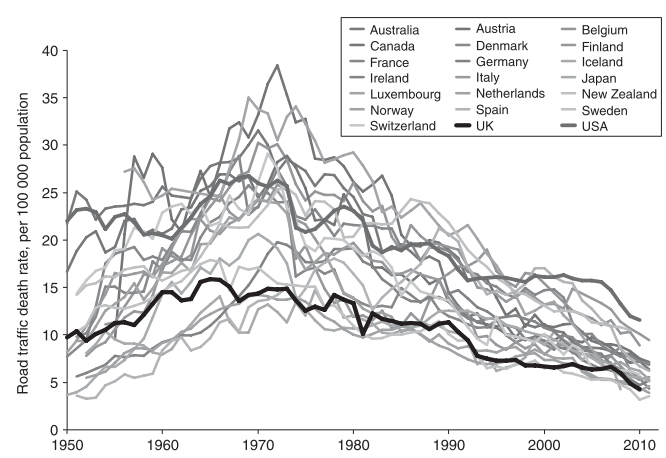
\includegraphics[width=0.8\textwidth]{fig/oecd.png}
    \label{fig:oecd}
    \par SOURCE: \textcite{Bhalla2016}.
\end{figure}

In the scope of economic determinism, road traffic deaths are defined as a process related to the country's development. The rising pattern is associated with the increase in motorization, and the decreasing pattern appears after a certain level of development is achieved, in other words, the countries have the means to implement effective investments in road safety. But this hypothesis has some flaws. This creates an impression that LMICs are not able to invest in road safety before becoming fully developed, which is inaccurate. Also, this idea shifts the focus on investment in direct interventions, encouraging the countries to focus on income growth as a strategy for road safety \cite{Bhalla2016}.

As mobility, in general, becomes more motorized towards car use, pedestrians start shifting into car users. This circumstance is known as risk substitution, where the increase in car users occurs at the same time as the number of pedestrians declines, lowering the exposure to more severe road traffic injuries like the collision between cars and pedestrians and lowering the number of road traffic deaths. However, this phenomenon can be imprecise when considering the motorization of LMICs, in which mass transit, motorcycles, and other non-motorized transportation means have a greater role on the vehicle fleet \cite{Bhalla2016}.   

A factor that explains this pattern in a more precise way is the political shift in the road safety paradigm that happened in the OECD countries. Before the 1950s, the belief that drivers were the only ones responsible for road crashes lead the discussions regarding road safety. Therefore, most of the interventions in road safety management ignored the design and development of the built environment and the vehicles. Between the 1960s and the 1970s, OECD countries started to regulate transport to tackle the road safety problems that were rising, establishing new laws and road safety management institutions on national and local levels. \cite{Bhalla2016}. Analyzing the road safety data from Brazil, it is possible to correlate the current stage with the stage experienced by the OECD countries during the 1970s.

According to \textcite{WHO2018}, it was predicted that Brazil would have a road traffic mortality rate (number of deaths per 100,000 inhabitants) of 22.5 in 2016, the highest rate among the South American countries. In 2019, road crashes were responsible for 31,945 deaths. Considering the Decade of Action for Road Safety 2011-2020 \cite{WHO2011}, Brazil reached the goal of reducing the road traffic deaths by half (comparing to the number projected for 2020, in case of a rising trend in deaths) by the end of the 2010s. \autoref{fig:br_abs} contains the time series of road traffic deaths in the last decades.  

\begin{figure}[!htbp]
    \centering\footnotesize
    \captionsetup{font=footnotesize}
    \caption{ROAD TRAFFIC DEATHS IN BRAZIL}
    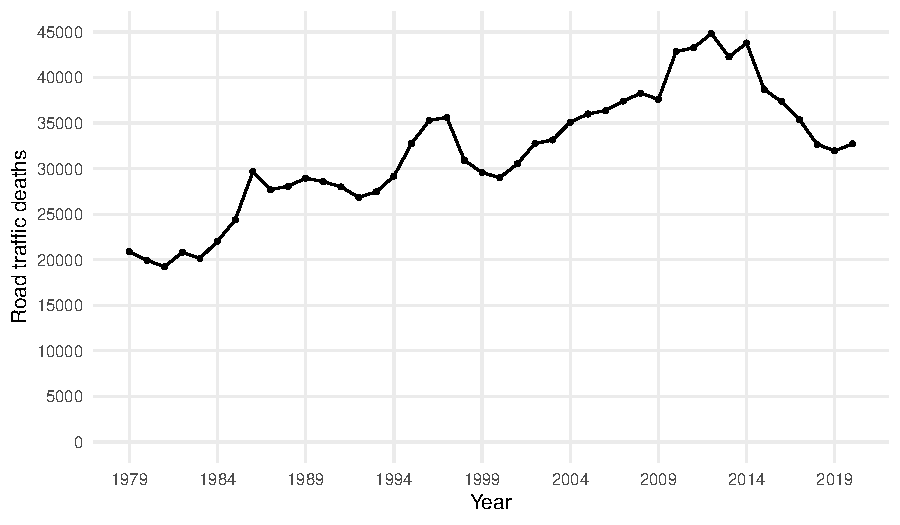
\includegraphics{fig/brazil_abs.pdf}
    \label{fig:br_abs}
    \par SOURCE: The Author (2022), based on \textcite{MinistryofHealth2020}.
\end{figure}

The year 1979 is the earliest official data entry available. Starting in the 1980s, there is an overall rising trend in the number of road traffic deaths, that reach its peak in 2012, then it starts to decline. In 2010, the year before the Decade of Action, Brazil had 42,844 deaths and reached the maximum value in 2012: 44,812 road traffic deaths. Almost at the end of the decade, the number of deaths declined, reaching 31,945. The next plot (\autoref{fig:br_mort}) includes a time series of the mortality rate in Brazil, considering the same period. In general, it follows the same pattern of absolute road traffic deaths.

\begin{figure}[!htbp]
    \centering\footnotesize
    \captionsetup{font=footnotesize}
    \caption{ROAD TRAFFIC MORTALITY RATE IN BRAZIL}
    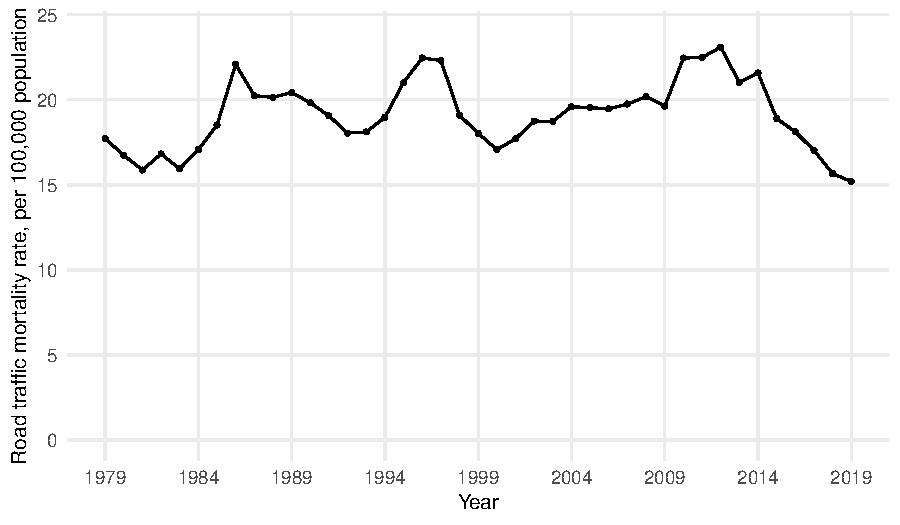
\includegraphics{fig/brazil_mort.pdf}
    \label{fig:br_mort}
    \par SOURCE: The Author (2022), based on \textcite{MinistryofHealth2020, MinistryofHealth2021}. 
\end{figure}

The maximum registered mortality rate is 23.1 deaths per 100,000 inhabitants in 2012, the same year in which Brazil reached its maximum value for absolute road traffic deaths. Since then, the mortality rate has been declining, reaching a rate of 15.2 deaths per 100,000 inhabitants in 2019. In comparison to the OECD countries (\autoref{fig:oecd}), Brazil presented a strong decreasing pattern a few years later, after the 2010s. Another indicator that considers the exposition to traffic hazards is the fatality rate – the number of deaths per 10,000 vehicles (\autoref{fig:br_fatal}). The oldest entry of fleet size in the \textcite{DENATRAN2020} database is 1998.

\begin{figure}[!htbp]
    \centering\footnotesize
    \captionsetup{font=footnotesize}
    \caption{ROAD TRAFFIC FATALITY RATE IN BRAZIL}
    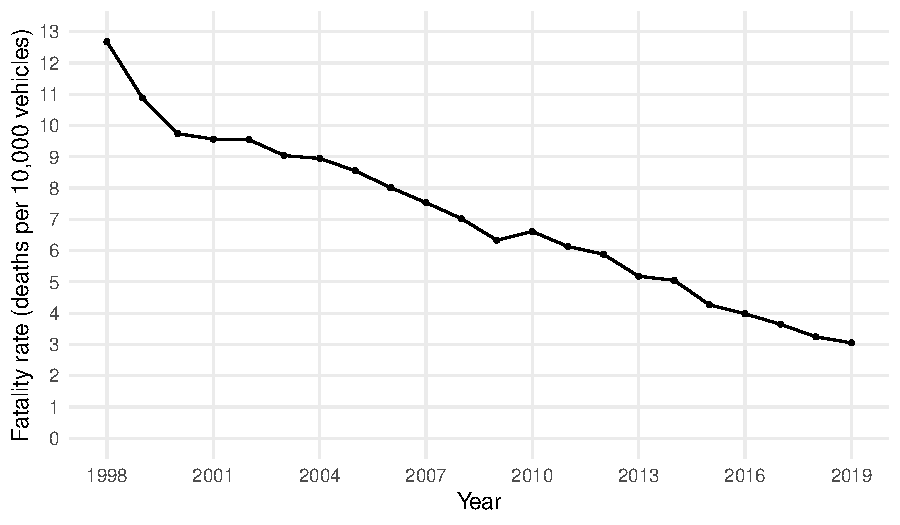
\includegraphics{fig/brazil_fatality.pdf}
    \label{fig:br_fatal}
    \par SOURCE: The Author (2022), based on \textcite{MinistryofHealth2020} and \textcite{DENATRAN2020}.
\end{figure}                                

Between 1998 and 2019 there is a declining pattern in the fatality rate, starting with 12.7 deaths per 10,000 vehicles in 1998 and ending with 3.0 in 2019, representing a reduction of 76\%. This declining pattern can be explained by the continuous rise of the motorization rate (\autoref{fig:br_motor}). In 1998, motorization rate was 151 vehicles per 1,000 inhabitants, increasing to the rate of 499 in 2019. Motorization can be defined as one indicator of development in the country. Considering the motorization stages defined by \textcite{Jorgensen2005}, Brazil can be classified nowadays with exploding motorization. 

The first stage of motorization – developing motorization – occurs when a country has a motorization rate between 50 and 100 vehicles per 1,000 inhabitants. This first stage happened in Brazil before 1998. The explosion of the motorization is the second stage, and it happens with a motorization rate of between 300 and 400. The third and the last stage is saturation and occurs when the motorization rate reaches more than 400 and its tendency stops rising \cite{Jorgensen2005}. Although Brazil has a present motorization rate above 400, it is plausible to state that the country still hasn't reached the stage of saturation, considering that the rates are still through a rising pattern. 

%% Create a plot with different types of vehicles.

\begin{figure}[!htbp]
    \centering\footnotesize
    \captionsetup{font=footnotesize}
    \caption{MOTORIZATION RATE IN BRAZIL}
    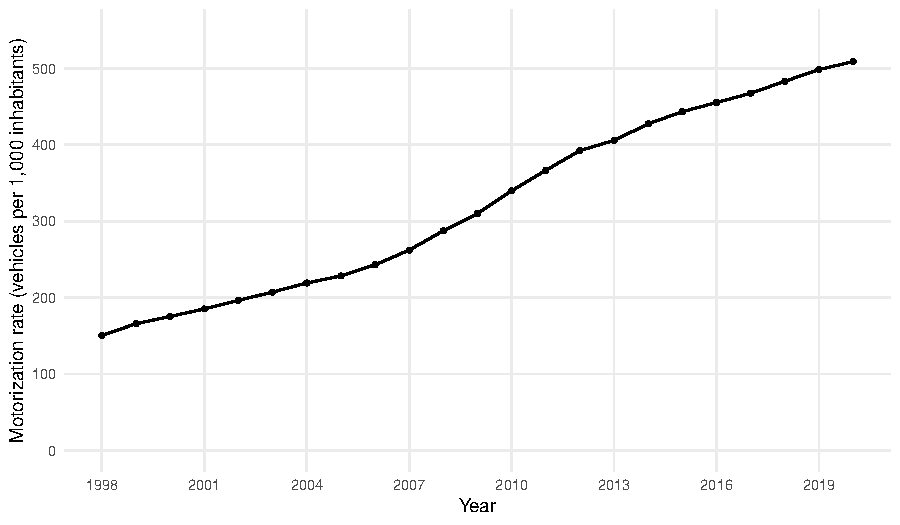
\includegraphics{fig/brazil_motor.pdf}
    \label{fig:br_motor}
    \par SOURCE: The Author (2022), based on \textcite{MinistryofHealth2021} and \textcite{DENATRAN2020}.
\end{figure} 

The evolution of Brazil's fleet size between 1998 and 2019 is presented in \autoref{fig:br_fleet}. Between 2007 and 2018, the quantity of vehicles in the country doubled. Car is the type of vehicle with the most quantity in all years presented in the time series. Motorcycle comes in second, followed by the quantity of trucks. In 2019, 66\% of the vehicle fleet was composed of cars. Motorcycles represented 27\% of the fleet, followed by trucks (3\%), other (3\%) and buses (1\%). 

\begin{figure}[!htbp]
    \centering\footnotesize
    \captionsetup{font=footnotesize}
    \caption{VEHICLE FLEET SIZE AND TYPE IN BRAZIL}
    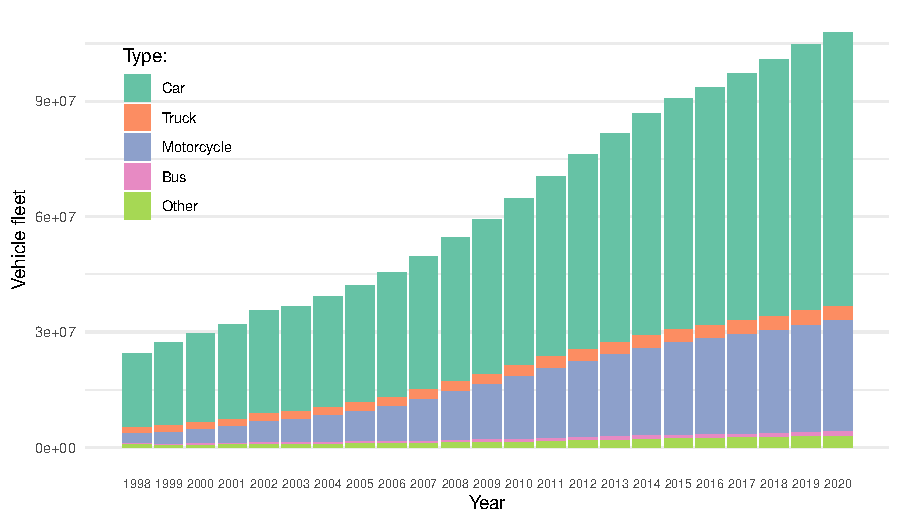
\includegraphics{fig/brazil_fleet_type.pdf}
    \label{fig:br_fleet}
    \par SOURCE: The Author (2022), based on \textcite{DENATRAN2020}
\end{figure}

Considering road crashes in federal highways, occurrences as a consequence of speeding are presented in \autoref{fig:prf_speed}. The earliest official data entry made available by the Federal Highway Police (PRF) is the year 2007, and the latest is 2020. In 2007, 6,011 road crashes happened as a consequence of speeding. The highest value of the time series happened in 2013, with 18,694 road crashes. In 2020, the number of road crashes reduced to 5,886. Regarding road crashes related to speeding in urban environments, it was not possible to find a database with this information. 

\begin{figure}[!htbp]
    \centering\footnotesize
    \captionsetup{font=footnotesize}
    \caption{ROAD CRASHES AS A CONSEQUENCE OF SPEEDING ON BRAZILIAN HIGHWAYS}
    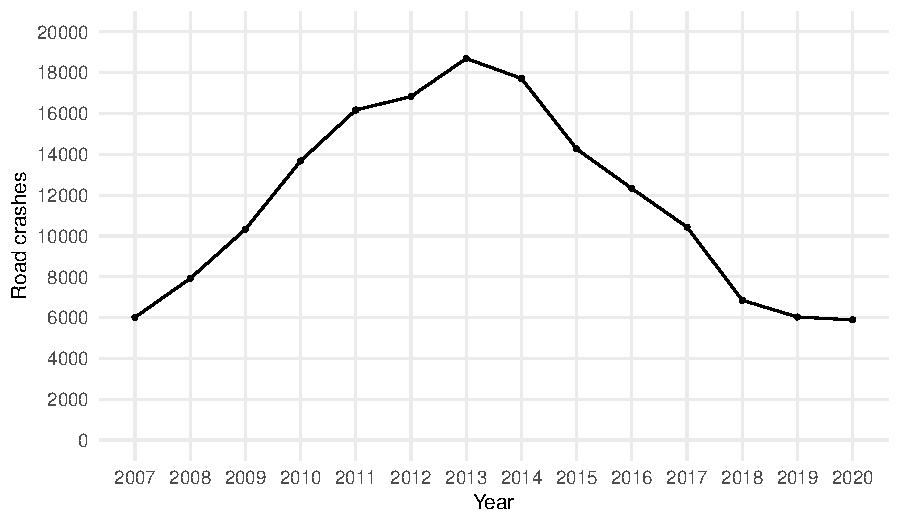
\includegraphics{fig/prf_plot.pdf}
    \label{fig:prf_speed}
    \par SOURCE: The Author (2022), based on \textcite{PRF2021b}
\end{figure}

In the 1970s, Brazil has undergone through intense development in the car industry, lowering the price of vehicles and increasing the development of road infrastructure in cities and rural areas. It produced a direct impact on the rise of motorization in the country \cite{Vasconcellos2013}. According to \textcite{Harvey1982}, this incentive to motorization created an urban environment that was planned to answer the increasing demand for car use. This process lead to worse safety conditions in Brazilian cities, especially for non-motorized users in the road system.   

The variation in the number of road traffic deaths and road traffic mortality is heavily influenced by the socio-economic development and political landscape \cite{Ferraz2012}. The country had different economical situations between the 2000s and the 2010s. From 2000 to 2010, Brazil had continuous economic growth, which was reflected in the rising pattern of road traffic deaths and road traffic mortality rates. After 2010, the country entered into an economic recession, leading to the reduction of these numbers \cite{Bastos2020}. Focusing on the area of study, the road traffic deaths in Curitiba are presented in \autoref{fig:cwb_abs}.   

\begin{figure}[!htbp]
    \centering\footnotesize
    \captionsetup{font=footnotesize}
    \caption{ROAD TRAFFIC DEATHS IN CURITIBA}
    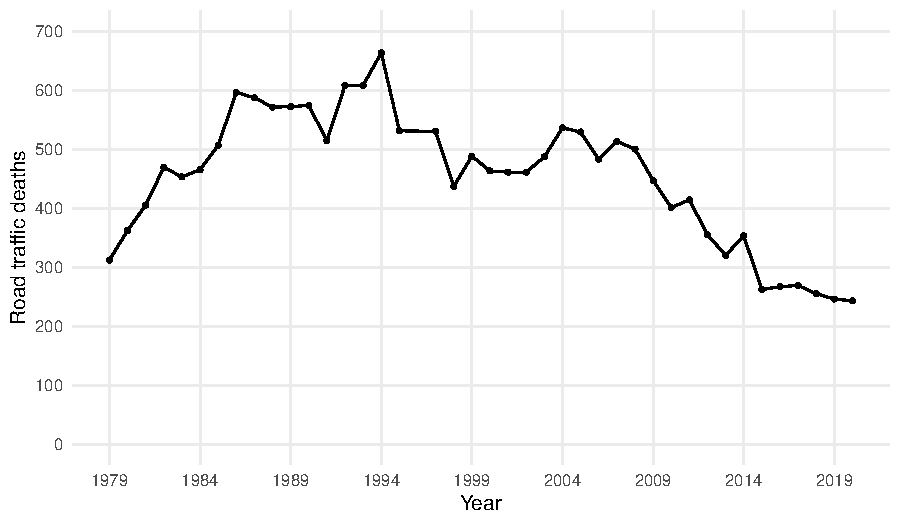
\includegraphics{fig/cwb_abs.pdf}
    \label{fig:cwb_abs}
    \par SOURCE: The Author (2022), based on \textcite{MinistryofHealth2020}.
\end{figure}  

The tendency of road traffic deaths presented a rising pattern between 1979 and 1994, starting with 312 deaths and reaching a maximum of 663 deaths. Overall, the pattern of the time series started declining after 1995, ending with a minimum value of 246 in 2019. Following the Brazilian trend, Curitiba's motorization rate kept rising in the last decades. The increase in motorized transit can lead to more exposition to traffic crashes and injuries, in case road safety interventions are not implemented correctly. The plot in \autoref{fig:cap_motor} compares the motorization rate between all Brazilian states' capital cities.    

\begin{figure}[!htbp]
    \centering\footnotesize
    \captionsetup{font=footnotesize}
    \caption{MOTORIZATION RATES IN BRAZILIAN STATES CAPITAL CITIES, IN 2019}
    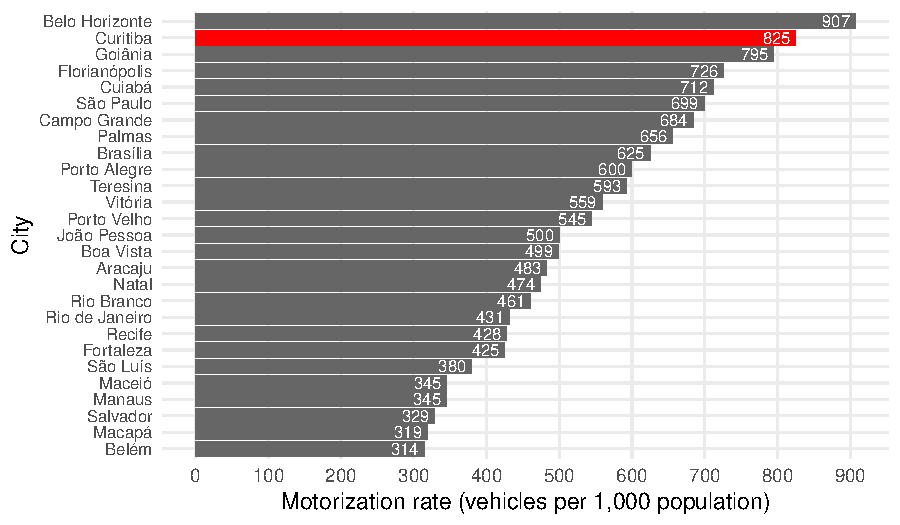
\includegraphics{fig/cap_motor.pdf}
    \label{fig:cap_motor}
    \par SOURCE: The Author (2022), based on \textcite{MinistryofHealth2021} and \textcite{DENATRAN2020}.
\end{figure}   

Curitiba was, in 2019, the second most motorized capital in Brazil, with a motorization rate of 825 vehicles per 1,000 inhabitants, higher than the Brazilian average of 499 vehicles per 1,000 inhabitants, only behind Belo Horizonte, which presented a motorization rate of 907 vehicles per 1,000 inhabitants. When comparing the road traffic mortality rate (\autoref{fig:cap_mort}), Curitiba stays in the 13th place between the capitals, with 12.7 deaths per 100,000 inhabitants, below the Brazilian average of 15.2 in 2019. The lowest value of road traffic mortality rate belongs to Rio de Janeiro, presenting a rate of 5.7 deaths per 100,000 inhabitants, and the highest belongs to Palmas, with an alarming rate of 36.4. In 2015, Curitiba had a mortality rate of 13.94 deaths per 100,000 inhabitants, a substantially high value when comparing to more developed countries, like Sweden (2.8), the UK (3.1), and Germany (4.1). Curitiba's rate for 2015 has a similar value to other Latin American countries: Mexico (13.1), Uruguay (13.4), Peru (13.5), and Argentina (14.00) \cite{WHO2018}. 

\begin{figure}[!htbp]
    \centering\footnotesize
    \captionsetup{font=footnotesize}
    \caption{MORTALITY RATES IN BRAZILIAN STATES CAPITAL CITIES, IN 2019}
    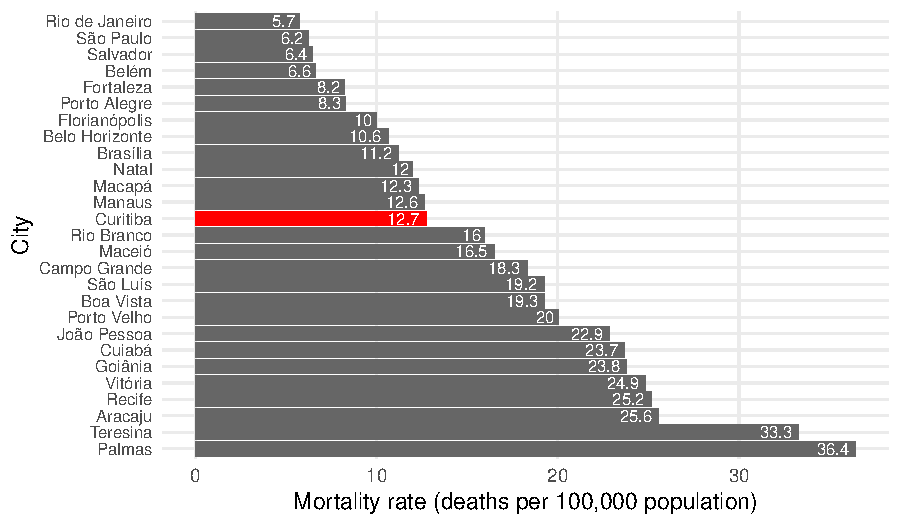
\includegraphics{fig/cap_mort.pdf}
    \label{fig:cap_mort}
    \par SOURCE: The Author (2022), based on \textcite{MinistryofHealth2020,MinistryofHealth2021}.
\end{figure}  

The evolution of vehicle fleet size in Curitiba is shown in \autoref{fig:cwb_fleet}. Following the Brazilian trend (\autoref{fig:br_fleet}), Curitiba's vehicle fleet is mostly composed of cars (82\%). Motorcycles represent 11\% of the fleet, followed by trucks (3\%), other (3\%) and buses (1\%). The car percentage in Curitiba's fleet is higher than the Brazilian average (66\%) for the same year, and the motorcycle percentage is lower (11\% vs 27\%).

\begin{figure}
    \centering\footnotesize
    \captionsetup{font=footnotesize}
    \caption{VEHICLE FLEET SIZE AND TYPE IN CURITIBA}
    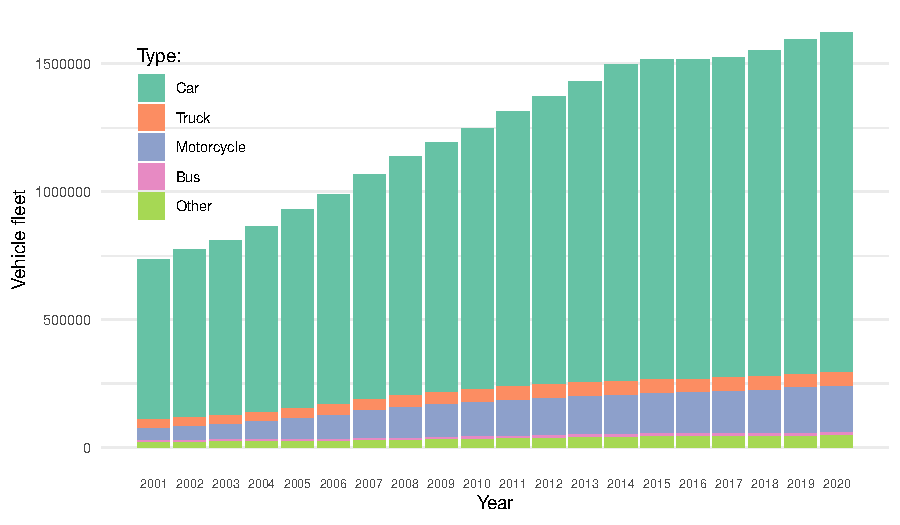
\includegraphics{fig/cwb_fleet_type.pdf}
    \label{fig:cwb_fleet}
    \par SOURCE: The Author (2022), based on \textcite{DENATRAN2020}
\end{figure}

Considering the fatality rate as a road safety performance indicator, Curitiba has the 6th best performance (\autoref{fig:cap_fatal}), with a fatality rate of 1.5 deaths per 10,000 vehicles. São Paulo is the capital with the lowest fatality rate (0.9) and Recife has the highest one (5.9). Observing the fatality rate in Brazil in the same period (3.0), Curitiba is below the country average, with exactly 50\% fewer deaths per 10,000 vehicles. Road traffic crashes and their related injuries have become a serious health problem across Brazilian cities. As motorization increases, the number of conflicts and possible crashes increases as well.

\begin{figure}[!htbp]
    \centering\footnotesize
    \captionsetup{font=footnotesize}
    \caption{FATALITY RATES IN BRAZILIAN STATES CAPITAL CITIES, IN 2019}
    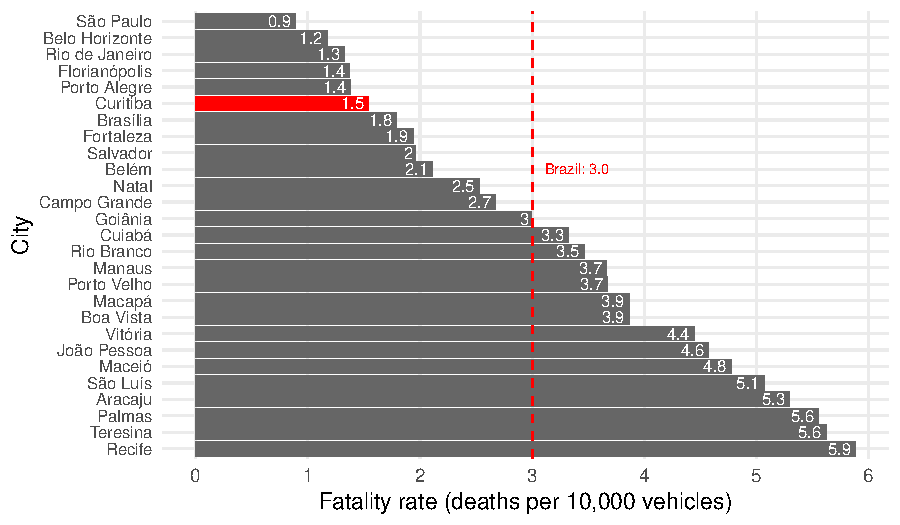
\includegraphics{fig/cap_fatal.pdf}
    \label{fig:cap_fatal}
    \par SOURCE: The Author (2022), based on \textcite{MinistryofHealth2020} and \textcite{DENATRAN2020}.
\end{figure} 

The road traffic deaths data made available by the \textcite{MinistryofHealth2020} do not only count the occurrences from road crashes that happened in Curitiba, but also consider the deaths that occurred in the city's hospitals and ambulances. Therefore, this data also can include deaths from crashes that happened outside Curitiba, but the rescue of the victim was carried out inside the city health system. To overcome this inaccuracy in the data, the municipal government of Curitiba has been compiling the data of road traffic deaths that happened only inside the city's territory since 2018, with the earliest entry in 2011 and the latest in 2020, as shown in \autoref{fig:pvt_deaths}.  

\begin{figure}[!htbp]
    \centering\footnotesize
    \captionsetup{font=footnotesize}
    \caption{DEATHS FROM ROAD CRASHES THAT HAPPENED IN CURITIBA}
    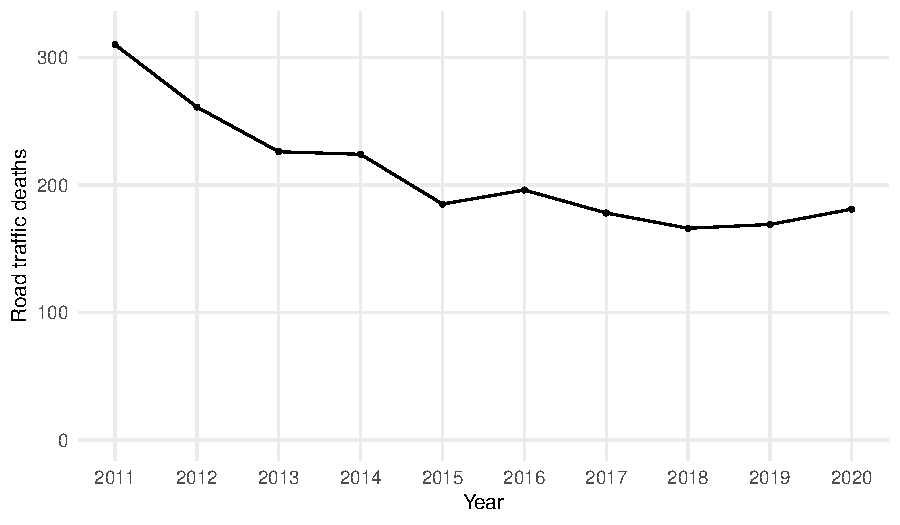
\includegraphics{fig/pvt_plot.pdf}
    \label{fig:pvt_deaths}
    \par SOURCE: The Author (2022), based on \textcite{Curitiba2021}.
\end{figure} 

According to \textcite{Curitiba2021}, 310 road traffic deaths occurred in 2011, the highest value of the time series. In 2018, the number of road traffic deaths reached its lowest value: 166. In the most recent entry, road traffic deaths reached a value of 181. Between 2011 and 2019, speeding was the second-highest causing factor of road traffic fatal crashes in Curitiba. The highest cause of fatalities was driving under influence \cite{Curitiba2020}. Between 2012 and 2020, pedestrian fatalities consisted of 37\% of total road traffic deaths, and cyclists' fatalities consisted of 8\% \cite{Curitiba2021}.

\section{ROAD SAFETY RISK FACTORS} \label{sec:risk}

Capable interventions in road safety need to consider traffic deaths and injuries as serious public health problems. Therefore, its control must follow the principle of control of any other public health problem. Road traffic injuries are the result of a complex interaction of multiple factors. These factors can involve human, environmental and vehicle factors, in addition to sociological, psychological, physical, and technological factors that are present in the process of traffic crashes. Like other health problems, it is possible to analyze road traffic injuries considering three different phases in time: pre-crash, during the crash, and post-crash \cite{Mohan2016}.

These distinct phases of time and factors of road traffic crashes can be arranged into a matrix created by \textcite{Haddon1980} to map all causes related to an injury. Named after its author, the Haddon matrix (\autoref{fig:haddon}) consists of two dimensions: one for the time aspect of the event and a second one representing three main factors: human, vehicle, and environment. Crossing each step of the two dimensions (factors and phases) leads to nine cells, in which a list of countermeasures to control the damage or to prevent a possible incident can be made, associating these measures to each pair of factors. 

\begin{figure}[!htbp]
    \centering\footnotesize
    \captionsetup{font=footnotesize}
    \caption{HADDON MATRIX}
    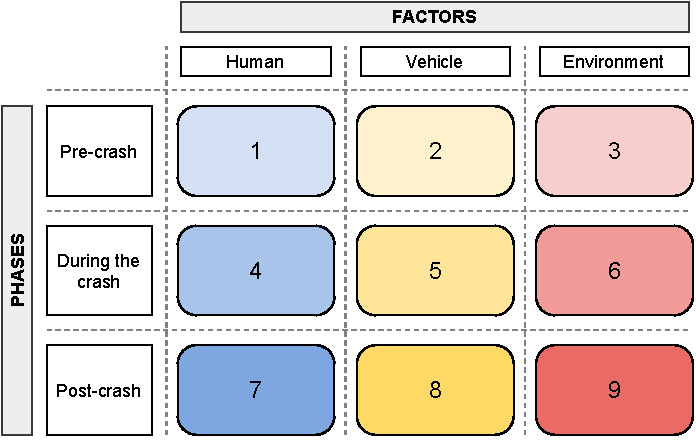
\includegraphics{fig/haddon.pdf}
    \label{fig:haddon}
    \par SOURCE: The Author (2022), based on \textcite{Haddon1980}.
\end{figure} 

Cells 1, 2, and 3 contain measures towards the prevention of crashes. On a road traffic crash scenario, cell 1 considers the behavior (e.g., aggressive driving, driving under influence, distraction) and training of the road users (e.g., pedestrians, drivers, motorcyclists, and cyclists), cell 2 presents safety interventions related to the vehicles (e.g., use of daylight headlights, speed control systems, etc.) and cell 3 contains all elements of the road infrastructure and build environment that influences directly into the occurrence of this event. Cells 4, 5, and 6 comprehend measures that can reduce the severity during the occurrence of a crash event.

In cell 4 some measures include the use of seat belts, helmets, and protective clothing. Cell 5 considers the crash worthiness and safety design of the vehicles and cell 6 includes elements (or lack of elements) that can influence the severity in case of a collision (e.g., guard rails, concrete barriers, street furniture, etc.). In the last row, the measures related to the control and treatment of injuries after the event are included. Cell 7 presents the treatments related to the victims (e.g., hospital care and rehabilitation); cell 8 contains measures related to the safety systems of a vehicle and cell 9 considers the general management of a crash scene \cite{Mohan2016}. 

The road safety problems that happen in urban environments may differ from the ones that happen in major roadways. Even with lower operating speeds, the number of conflicts in urban road systems can be substantially higher when comparing to rural roadways, considering the quantity of different motorized and non-motorized transport modes that use the infrastructure at the same time. Consequently, it is essential to follow the requirements for safe infrastructure. The three main ones are functionality, homogeneity, and recognition \cite{SWOV2003}. Each road on a network needs to have a specific function (balance between mobility and access), with traffic distribution working as intended. Homogeneity consists in reducing the points of conflict between transport modes with a great difference of mass and speed. Finally, the situations on traffic should have a level of predictability, which consists of the road users' expected behavior. 

To reduce road traffic crashes and possible consequent injuries or deaths, it is relevant to consider the main risk factors that cause and intensify these events. According to \textcite{WHO2004}, the risk in road traffic can be classified into four elements that are directly influenced: exposure, crash involvement, crash severity, and post-crash severity. The risk factors that can be classified in these elements also can be distributed within the Haddon matrix as well (\autoref{fig:haddon}). The main risk factors related to the protection of the user consist of the usage of seat belts, helmets, airbags, child restraints, and helmets. Focusing on the behavioral factors, the main ones are driving under influence of alcohol and other drugs (DUI), distraction, and inattention \cite{Shinar2017}.

The Safe System Approach is a framework that aims to develop road systems that establish a better management of crash forces, being able to accommodate human error in a way that is not fatal for the users \cite{international_transport_forum_towards_2008}. In this framework, the road safety interventions previously described are maintained and intensified, added to a safety management process that integrates key aspects of road user behavior, traffic environment, speed management and vehicle systems for the increase in road safety performance. According to \textcite{larssonSafeSystemApproach2013}, road safety interventions in the Safe Systems does not treat the human error as an individual error, but as system's failure. A more recent framework for developing safer environments is the Safe System Approach. 

Considering that this failure will continue to occur, the safe system focus on prevention of serious injuries and deaths. Therefore, the design of the road system should guide the users to a safer behavior, mitigating more severe outcomes. The physical vulnerability of the human body is at the center of the Safe System Approach. Speed limits and road infrastructure must be compatible to this tolerance. The safe systems evolve from traditional approaches to safety problems, not relying on how well the road users performs their tasks. The design of the road transport system should guide the road user to a safer speed levels, mitigating possible crashes and injuries \cite{international_transport_forum_towards_2008,wegmanFutureRoadSafety2017}. 

The excess of speed and the speed differential in urban environments are two risk factors that affect the chance of traffic crashes occurrence and the severity of these crashes. Speed differential is the disparity of speeds between vehicles on the same road, leading to higher chances of conflicts. Speeding, which consists of exceeding the speed limit of a road, is a complex phenomenon with multiple causes, consequences, and methods of prevention. Given its complexity, this risky behavior is discussed in the next section (\ref{speeding}). 

\section{SPEEDING AS A RISK FACTOR} \label{speeding}

Speeding is one of the primary global causes of road traffic fatalities, affecting two main dimensions: probability and severity \cite{WHO2013}. The increase in vehicle speeds is directly correlated to the increase in the occurrence of crashes and their average severity, hence, strongly related to road safety \cite{Mohan2016a}. Another speed-related risk factor is the speed differential, which is the speed deviation from the average operating speed \cite{Shinar2017}. \textcite{Ferraz2012} define speeding as an inappropriate speed, leading to more conflict and crashes in certain traffic conditions. 

The excess of speed can influence three main aspects in the occurrence of a traffic conflict: reaction time, braking distance, and force of impact, which is directly correlated to the severity of injuries \cite{Mohan2016a}. Reducing the speed helps the driver to increase its reaction time, and to take correctional action to anticipate crashes \cite{Elvik2009}. Regarding the braking distance, lower speeds reduce the distance necessary to fully stop the vehicle. In \autoref{fig:braking}, it is possible to verify the reaction time of a vehicle added to the braking distance, resulting in the distance traveled by the vehicle until the complete stop. The dashed line represents a pedestrian standing 35 meters from the moving vehicle. 

\begin{figure}[!htbp]
    \centering\footnotesize
    \captionsetup{font=footnotesize}
    \caption{RELATIONSHIP BETWEEN SPEED AND BRAKING DISTANCE}
    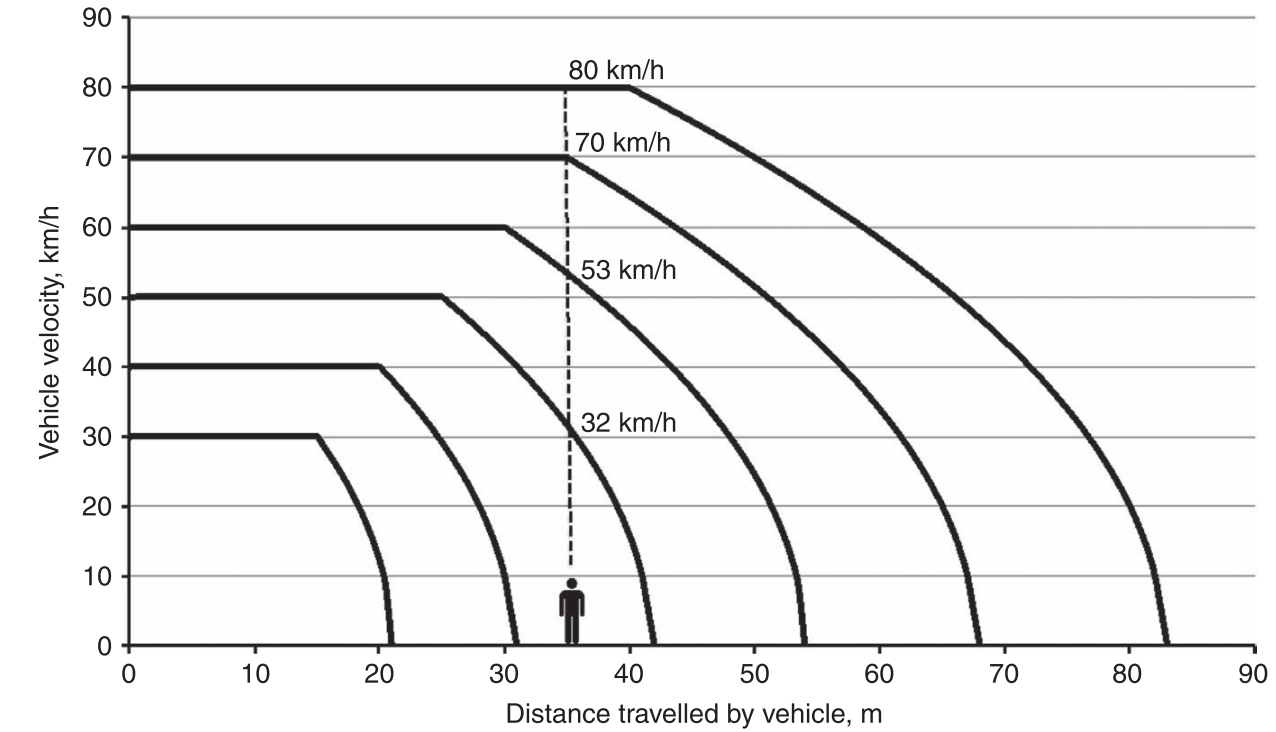
\includegraphics[width=0.8\textwidth]{fig/braking2.png}
    \label{fig:braking}
    \par SOURCE: \textcite{Mohan2016a}.
\end{figure} 

The horizontal lines from the plot show the cruising speeds of the vehicle before they start breaking, longer lines at higher speeds represent greater reaction times. In this scenario, only speeds equal to or below 40 km/h can avoid a collision with the pedestrian. As the vehicle speed rises, the impact speed rises as well. This leads to  an increase in the force of impact between vehicles and pedestrians. The severity of injuries sustained by pedestrians depends on the energy of impact – the kinetic energy transferred to the human body. This energy of an object (the vehicle) is directly related to its velocity and mass, detailed in the following equation: \begin{align}
    E = 0.5 \times MV^2 \mbox{;}
    \label{eq:energy}
\end{align} where $E$ is the kinetic energy, $M$ is the object's mass and $V$ is the velocity of the object. The plot in \autoref{fig:kinetic} shows the increase in kinetic energy, considering an average car mass of 1,500 kg \cite{Zervas2008} and speeds varying between 0 and 100 km/h. The quantity of energy doubles when the speed changes from 40 km/h to 60 km/h, and almost triples at 70 km/h. This variation shows how the reduction of speed limits can greatly change the energy of impact.

\begin{figure}[!htbp]
    \centering\footnotesize
    \captionsetup{font=footnotesize}
    \caption{RELATIONSHIP BETWEEN SPEED AND KINETIC ENERGY}
    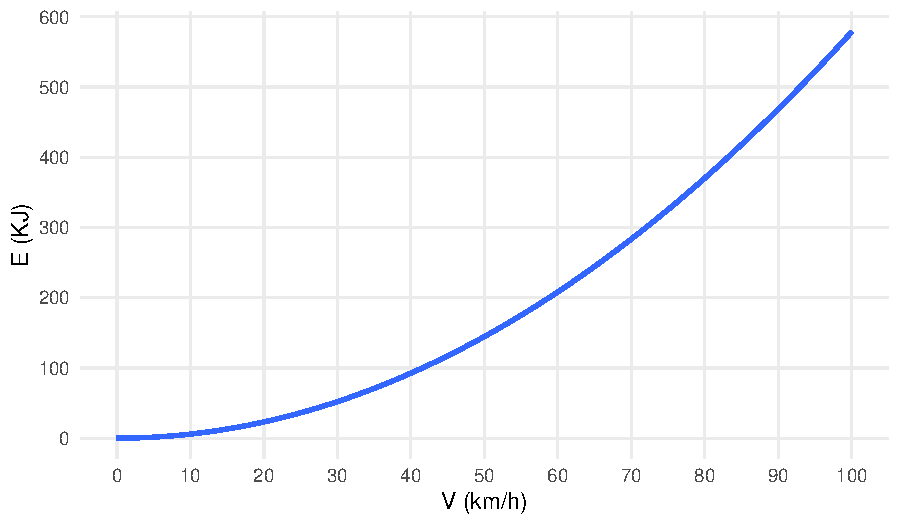
\includegraphics{fig/kinetic.pdf}
    \label{fig:kinetic}
    \par SOURCE: The Author (2022).
\end{figure}

Considering the event of an impact between the front of a car and a pedestrian, \textcite{Ashton1980} presented the relationship between the impact speed and the percentage of fatally injured pedestrians per speed window, represented in the plot of \autoref{fig:ash}. The curve shows how a reduction from 60 km/h to 40 km/h on the speed of impact can reduce the chance of a fatal injury from 90\% to 30\%, approximately. Reducing the speed of impact to 30 km/h will reduce the chance of a fatal injury to approximately 10\%. In general, as the speed of impact rises, the chance of a fatal injury rises too, with a greater variation between speeds of 30 km/h and 60 km/h. 

\begin{figure}[!htbp]
    \centering\footnotesize
    \captionsetup{font=footnotesize}
    \caption{PROBABILITY OF PEDESTRIAN FATALITY AT DIFFERENT IMPACT SPEEDS}
    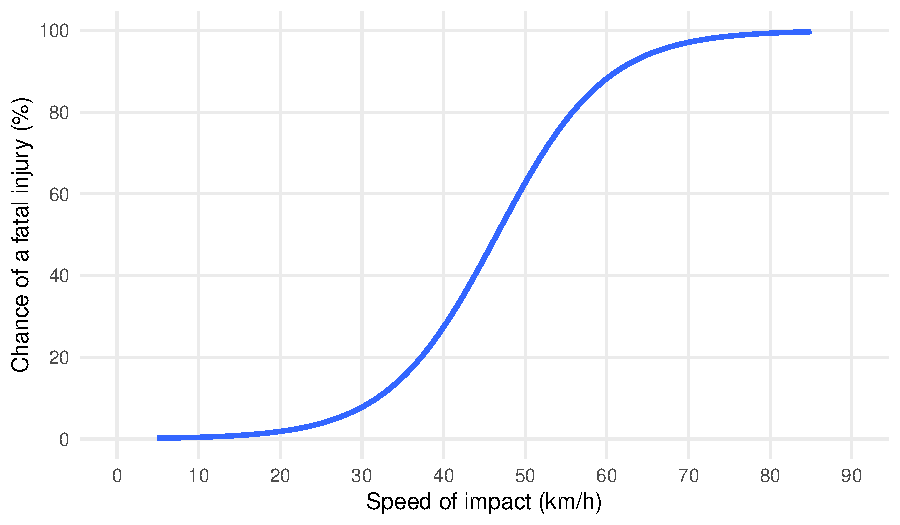
\includegraphics{fig/ash.pdf}
    \label{fig:ash}
    \par SOURCE: The Author (2022), based on data from \textcite{Ashton1980}.
\end{figure}

The risks related to speeding behavior highlight the importance of proper speed management in road traffic, especially in urban environments. Roadways have higher operational speeds, but cities contain a more expressive interaction between motorized and vulnerable users, in which even lower speeds can still represent a risk to pedestrians and cyclists. One method to manage the operating speed is the enforcement of speed limits. It is recommended a speed limit of 30 km/h in areas where there are a great number of interaction between vulnerable road users and vehicles, except where strong evidence exists that higher speeds are safe \cite{WHO2020,whoGlobalPlanDecade2021}. Reducing the mean speeds can greatly favor the decline in fatal, non-fatal, and property damage only (PDO) road crashes \cite{Elvik2013}. In Brazil, speed limits in cities are defined based on the category of road hierarchy. In decreasing order, rapid transit roads have a limit of 80 km/h, followed by arterial roads, with a limit of 60 km/h; collector roads – 40 km/h; and local roads, with a limit of 30 km/h \cite{Brasil1997}.

The operating and mean speed of the road traffic depends on how drivers choose the speed. This choice is related to the power and stability of the user's vehicle, to road and traffic conditions, to driver's perception of safety, to the level of enforcement, to travel motivations, to personal characteristics, and to the behavior of other drivers \cite{Mohan2016a, Shinar2017}. Considering all these factors, it is not effective to rely only on traffic limits to prevent speeding. If the design speed of a road is higher than the speed limit and the road traffic has a low density, it is more difficult to avoid the driver to reach the desired speed. The difficulty to enforce the speed limits may be higher in LMICs, where there are fewer resources to adopt the proper road designs policies and lower enforcement available required to this task \cite{Mohan2016a}. 

In \autoref{tab:spdfct} a few groups of factors affecting speeding and speed choice are presented, with its categorization based on the three main discrete factors of road crashes established by \textcite{Haddon1980}: human, vehicle and environment. Analyzing the human (or driver) factors, the background characteristics include the level of experience, education, and training of the drivers. Demographic characteristics consider the groups of age, gender, and income. The general health of the driver, including the conditions of vision, hearing, and sleep patterns, are included in the physiological factors. The last factor in the human group – attitudes, beliefs, and motivations considers how the road user perceives the control and norms present in traffic situations \cite{Richard2013a}.  

\begin{table}[!hbtp]
    \footnotesize
    \captionsetup{justification=raggedright,
        singlelinecheck=false,
        font=footnotesize}
    \caption{FACTORS THAT AFFECT SPEEDING AND SPEED CHOICE}
    \centering
    \begin{tabular}{lll}
    \hline
    \multicolumn{1}{c}{\textbf{Human}}                  & \multicolumn{1}{c}{\textbf{Vehicle}} & \multicolumn{1}{c}{\textbf{Environment}} \\ \hline
    Background characteristics      & Type/Size        & Road elements        \\
    Demographic characteristics     & Engine power     & Weather              \\
    Physiological factors           & Comfort          & Traffic conditions   \\
    Attitudes, beliefs, and motivations & Field of view    & Surroundings    \\
                                    & Age              & Speed Enforcement    \\ \hline
\end{tabular}
    \label{tab:spdfct}
    \par \vspace{2mm} \footnotesize \raggedright
    SOURCE: The Author (2022), based on \textcite{Richard2013a}, \textcite{Shinar2017}, and \textcite{WHO2008}.
\end{table}

All these human factors are related to the general driver profile and its performance when driving the car. As an example of the influence of the individual differences present in the demographic characteristics, younger drivers are more likely to speed than mature and older drivers; and men are more likely to speed than women \cite{Shinar2017}. The vehicle characteristics also affect the speed choice of the user. The type, engine power, comfort, field of view, and age of the vehicle can affect the possibility of the driver to reach the desired speed. 

The environmental factors affecting speed choice consist of all the elements external to the vehicles and are greatly related to how the driver behaves and to how the vehicle can operate. Road elements can include the general characteristics of a road layout, quantity, and type of intersections, design, and level of maintenance, based on its alignment, gradient, width, surface condition, geometric pattern, and road lighting. The presence of intersections and the high density of traffic controls the operating speeds in urban areas \cite{Mohan2016a}. Weather can also affect how the driver will choose his speed, considering its effects on surface conditions (dry, wet, ice) and natural light.  

The speed and speed variance are to a certain extent determined by the traffic flow regime \cite{Shinar2017}. Depending on the level of flow and density or any other operational condition of the traffic, the driver cannot be able to reach a higher desired speed, removing his ability to have an opportunity to speed \cite{Richard2013a, Bastos2021}. The plot in \autoref{fig:svd} illustrates the relationship between speed, density, and volume (or flow) in uninterrupted flow conditions of a certain road. This relationship was modeled by \textcite{Greenshields1934} and named after its author. This type of flow occurs in areas without interference from external factors, like intersections or crossings \cite{Green2020}. 

\begin{figure}[!htbp]
    \centering\footnotesize
    \captionsetup{font=footnotesize}
    \caption{GREENSHIELDS MODEL}
    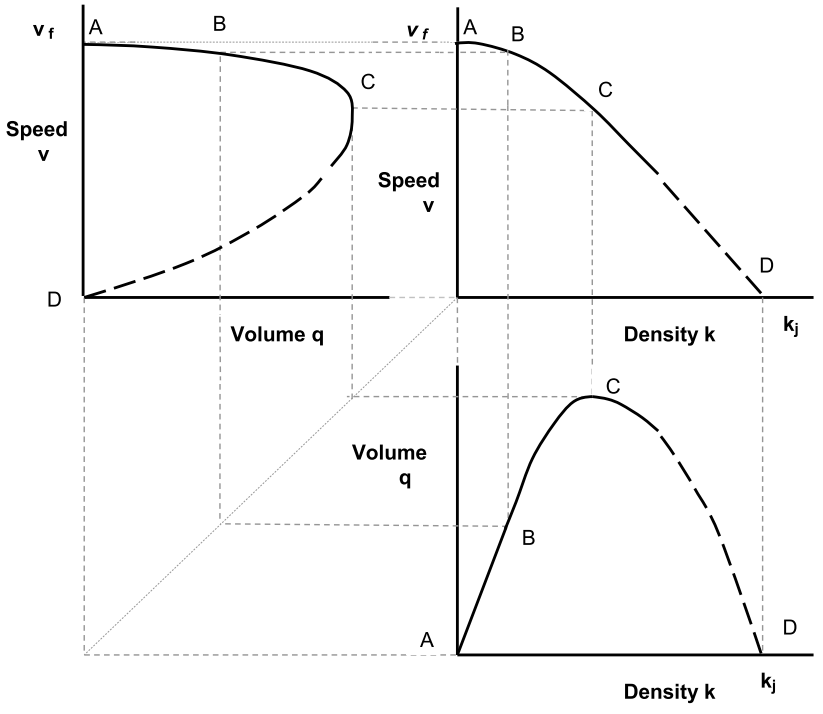
\includegraphics[width=0.8\textwidth]{fig/svd.png}
    \label{fig:svd}
    \par SOURCE: \textcite{Green2020}, based on \textcite{Greenshields1934}.
\end{figure}

When density and volume are at their lowest value, the road user can reach higher speeds without having traffic to prevent it (point A). Between points A and B, volume and density rise, and speeds decline a little but still are high enough to be characterized as a free-flow speed. In this situation, the driver starts to experience a lack of maneuver freedom, but it still has the opportunity to speed. At the highest level of density (point C), speed declines as density rises. Between C and D, density rises until it reaches its maximum value, reducing the overall traffic stream speed and flow \cite{Green2020}. In this last stage, the drivers have less flexibility to choose the desired speed, having to operate in a forced flow condition. 

Established as an environmental factor affecting speeding choice (\autoref{tab:spdfct}), the surroundings of the road, including equipment and some traffic-calming techniques like gateway treatments can be perceived by the driver as elements that give hints to avoid higher speeds \cite{WHO2008}. Overall, the built environment and its five elements – density, design, diversity, destination accessibility, and distance to transit – can be perceived as environmental factors which affect road safety, through the relationship to the number of road crashes and occurrence of speeding. These characteristics are better explored in the next section (\ref{be}). 

To collect speeding data and to compute a reliable road safety performance indicator, it is important to establish what defines speeding and to identify a measure of exposure to speeding. To \textcite{Richard2013}, defining speeding and its constitution is one of the key challenges of speeding studies. The authors presented five distinct approaches for speeding definition: \textit{ad hoc}, analytical, kinematic, psychological, and behavioral. The ad hoc approach assumes that the fastest driving in a sample is a proxy for speeding, and considers the top $X\%$ of speeds above the speed limit. Although this approach can provide sufficient data for analysis, the speeding collected might not be related to behavior or safety. 

The analytical approach fixes a criterion relative to the speed limit ($+ X\%$ or $+ X km/h$). It is a simple method to implement, but can miss some factors related to road type and overall speed level. The analytical approach is used in this work and its process of implementation is detailed in Section \ref{data}. The kinematic approach considers the driving environment and its operational conditions, to connect the speed behavior to specific situations. This approach requires a certain level of quantity and quality of GIS data to support it. The psychological approach is based on what the driver considers to be speeding, providing insight into factors that are related to an individual's perception of speeding. The need for additional previous information about the speeding beliefs and attitudes of the drivers can be a disadvantage of this approach. At last, the behavioral approach sets four speed bands to describe different behavior in each one, related to the chosen speed by the driver \cite{Richard2013}.

The operational aspects of urban road traffic (mostly in interrupted flow conditions) arbitrarily reduce the amount of speeding being measured. To address this problem, it is necessary to extract the free-flow situations of the trip from the total trip distance, removing situations in which drivers had no opportunity to speed. This process of extracting parts of the trip in which the driver is exposed to speeding is presented in \autoref{fig:ff}. Therefore, the actual measure of speeding is distance performed in speeds above the speed limit compared to the distance performed in free-flow speed. This process was applied in this work, and it is described in Section \ref{data}. 

\begin{figure}[!htbp]
    \centering\footnotesize
    \captionsetup{font=footnotesize}
    \caption{EXTRACTION OF FREE-FLOW AND SPEEDING EPISODES FROM TRIPS}
    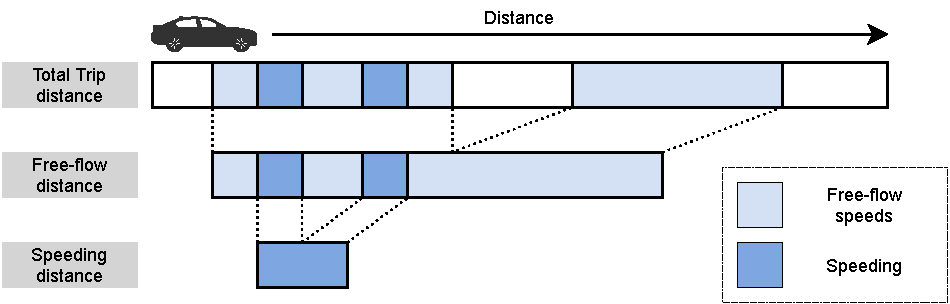
\includegraphics{fig/richards.pdf}
    \label{fig:ff}
    \par SOURCE: The Author (2022), based on \textcite{Richard2013}.
\end{figure}

The collected data also depends on the method applied. The collection of speed data can be done with the use of speed traps – fixed or mobile \cite{Hidalgo-Solorzano2020, WHO2008}, the analysis of road crashes reports \cite{Watson2015}, roadside observational studies \cite{Shinar2017}, questionnaires \cite{Dinh2013}, smartphone data \cite{Warren2019} and GPS data collection \cite{Moreno2013, Wang2018}. Studies that use naturalistic data include the video recording data from the drivers and GPS data, which together can relate the speeding action registered with a certain behavioral action from drivers \cite{Bastos2020a} and environmental factors \cite{Moreno2013}. The speeding data collected from driving simulation studies can also be correlated with other environmental or behavioral factors \cite{Yadav2020}. The aspects of naturalistic driving studies and their comparison to other methods will be better explored in Section \ref{nds}. 

Through the knowledge of the factors that affect speeding and the methods to collect and analyze speeding data, it is possible to plan countermeasures to this risk factor in road traffic crashes. Following the categories established by \textcite{Haddon1980} and presented in \autoref{tab:spdfct}, these countermeasures can be classified into behavioral (human), vehicular and environmental approaches. Behavioral approaches include the education and training to teach speed awareness to drivers. Enforcement is also a behavioral approach. Enforcement by the police or other traffic authority is related to a greater rate of speed limit compliance, but it is a highly localized measure \cite{Shinar2017}. 

The vehicle approach to intervening in speeding practices includes speed limits and advisory systems in cars. Environmental approaches consist of direct changes in infrastructure, including traffic-calming measures, and policy approaches, including the establishment of speed limits and administrative actions. Speed bumps, lane narrowing, roundabouts, and rumble strips are some traffic-calming techniques that are capable to reduce speeds in urban environments \cite{Welle2016}. Key elements of urban design, including the built environment, also can influence in practice of speeding. This influence is discussed in Section \ref{be}

\section{ROAD SAFETY PERFORMANCE AND THE BUILT ENVIRONMENT} \label{be}

% 1. Introduce the section with Tiwari (2016) and Ewing (2009)

%% Ewing and dumbaugh diagram

%% Tiwari 

%% Ewing and Cervero, 2010

The built environment consists of physical elements and features, including the development pattern and the roadway design of a city. The built environment affects the physical activity inside the city, including overall mobility, road safety, and health. According to \textcite{Ewing2009}, the frequency and severity of road traffic crashes are related to the built environment through three mediators: traffic volume, traffic conflict, and traffic speed, as shown in \autoref{fig:ewing}. Therefore, the land use and transport plans influence the choice of destination, modal choice, travel distances, and routes, impacting road traffic safety \cite{Tiwari}.  

\begin{figure}[!htbp]
    \centering\footnotesize
    \captionsetup{font=footnotesize}
    \caption{BUILT ENVIRONMENT AND TRAFFIC SAFETY}
    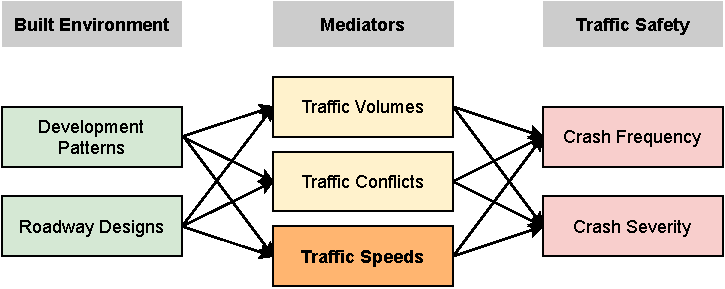
\includegraphics{fig/ewing.pdf}
    \label{fig:ewing}
    \par SOURCE: The Author (2022), based on \textcite{Ewing2009}.
\end{figure}

Traffic volume is directly related to the crash frequency and the increase of vehicle miles traveled (VMT), which is an exposure variable to the occurrence of road traffic crashes. Traffic speed (thus, speeding), the main factor investigated in this paper, is affected by the operating and encouraged speed defined by the roadway design and the development pattern. Traffic conflicts are related to the increase in vehicle flow and traffic speed \cite{Ewing2009}. Overall, the built environment can be characterized into five ``D'' variables: (\romannumeral 1) density, (\romannumeral 2) diversity, (\romannumeral 3) design, (\romannumeral 4) destination accessibility, and (\romannumeral 5) distance to transit, being defined as the 5D \cite{Ewing2010}. Demographics of residents, while not being part of the built environment, can be considered as the sixth ``D''. 

% 2. Describe the BE elements. (5D)

%% Table with 5D and elements used in this work

%% Other reports from Tiago

%% Tiwari

\autoref{tab:6d} contains the categories previously described and their corresponding variables. It is important to note that it is not presented all the possible built environment variables, only the main ones found in previous papers. In addition, these are rough categories, divided by boundaries that are subject to change \cite{Ewing2010}. Density measures a variable of interest per unit of area and can include the quantity of population, housing, or the number of jobs, showing the ``hotspots'' of the overall activity in a city. Diversity refers to different land use types within a given area, ranging from single-use environments to more varied land uses. The street network and its characteristics are included in the design category, and it considers elements like block size, type/quantity of intersections, street widths, the number of pedestrian crossings, and street network density.

\begin{table}[!hbtp]
    \footnotesize
    \captionsetup{justification=raggedright,
        singlelinecheck=false,
        font=footnotesize}
    \caption{BUILT ENVIRONMENT VARIABLES}
    \centering
    \begin{tabular}{ll}
        \hline
        \multicolumn{1}{c}{\textbf{Category}}                          & \multicolumn{1}{c}{\textbf{Variable}}                        \\ \hline
        \multirow{3}{*}{Density}                   & Population                               \\
                                                   & Housing                                  \\
                                                   & Employment                               \\ \hline
        \multirow{1}{*}{Diversity}                 & Land use                                 \\
                                                   \hline
        \multirow{6}{*}{Design}                    & Block size                               \\
                                                   & Type / Quantity of intersections                \\
                                                   & Street widths                            \\
                                                   & Quantity of pedestrian crossings         \\
                                                   & Road hierarchy \\
                                                   & Street network density \\
                                                    \hline
        \multirow{3}{*}{Destination Accessibility} & Quantity of commercial and service units \\
                                                   & Distance to city center                  \\
                                                   & Quantity of jobs                         \\ \hline
        \multirow{2}{*}{Distance to Transit}       & Quantity of bus stops                    \\
                                                   & Distance to the nearest transit stop         \\
                                                    \hline
        \multirow{3}{*}{Demographics}              & Income                                   \\
                                                   & Age                                      \\
                                                   & Sex                                      \\ \hline
        \end{tabular}
    \label{tab:6d}
    \par \vspace{2mm} \footnotesize \raggedright
    SOURCE: The Author (2022), based on \textcite{Ewing2009}, \textcite{Ewing2010} and \textcite{Obelheiro2020}.
\end{table}

Destination accessibility measures how easy it is to access places of attraction, including jobs, services, commerce, and districts of overall interest, considering business districts and city downtown. Distance to transit is usually measured by the supply level of transportation services, being measured by the number of transit stops and network density. Network density can also be included in the design category. Demographics, while not being a characteristic of the built environment itself, can influence the occurrence of speeding in urban environments, including income, age, and gender. In the following tables (\autoref{tab:density} to \autoref{tab:demographics}) the built environment categories and the variables considered in this work are presented, including the authors that investigated them related to the road safety performance in urban areas, with the focus on one final outcome indicator (road crashes) and one mediator (occurrence of speeding).

% 3. BE and relationship to road safety

%% table with all the authors

\autoref{tab:density} contains a list of authors who investigated the relationship between population density and road safety in urban areas. Regarding road traffic crashes, \textcite{Dumbaugh2009, Obelheiro2020} found an inverted correlation between the number of inhabitants per area and the occurrence of road crashes. Higher density environments cause people to drive less \cite{Dumbaugh2009}, reducing the exposure to road traffic accidents. Research considering road safety and BEs about another Southern Brazilian city – Porto Alegre – also presented a result of an inverted relationship between injury crashes and population density in most of the city's area.

\begin{table}[!hbtp]
    \footnotesize
    \captionsetup{justification=raggedright,
        singlelinecheck=false,
        font=footnotesize}
    \caption{CORRELATION BETWEEN DENSITY AND ROAD SAFETY OUTCOMES}
    \centering
    \begin{tabular}{llll}
        \hline
        \multirow{2}{*}{\textbf{Category}} & \multirow{2}{*}{\textbf{Variable}} & \multicolumn{2}{c}{\textbf{Road safety outcomes}} \\
         &  & \multicolumn{1}{l}{\textbf{Crashes}} & \multicolumn{1}{l}{\textbf{Speeding}} \\ \hline
        \multirow{6}{*}{Density} & \multirow{6}{*}{Population} & $(-)$ \textcite{Dumbaugh2009} & \multirow{6}{*}{---} \\
         &  & $(+)$ \textcite{Dumbaugh2013} &  \\
         &  & $(+)$ \textcite{Lee2015} &  \\
         &  & $(-)$ \textcite{Obelheiro2020} &  \\
         &  & $(+)$ \textcite{Pirdavani2014} &  \\
         &  & $(\pm)$ \textcite{Welle2016} &  \\ \hline
    \end{tabular}
    \label{tab:density}
    \par \vspace{2mm} \footnotesize \raggedright
    SOURCE: The Author (2022).
    \par \vspace{1mm} \footnotesize \raggedright
    NOTE: $(+)$: positive correlation between variable and outcome; $(-)$: inverted correlation between variable and outcome; $(\pm)$: correlation not clear / depends on other factors.
\end{table}

\textcite{Dumbaugh2013,Lee2015,Pirdavani2014} found a direct relationship between population density and the occurrence of road crashes. There is a positive relationship between population density and total pedestrian crashes \cite{Dumbaugh2013}, in addition to motor vehicle crashes and bicycle crashes \cite{Lee2015} and injury crashes \cite{Pirdavani2014}. According to \textcite{Welle2016}, higher density areas contain fewer motorized trips, which can reduce crashes involving cars, but can increase the number of conflicts within the area, therefore increasing the risk of overall crashes. Concerning the chance of speeding occurrence, a study relating population density as a BE variable to the speeding practice could not be found. Most authors investigate the speeding occurrence as a risk factor for these crashes. The statistical relationship between BE variables and the occurrence of motor vehicle speeding still needs to be better explored. It can be assumed that higher density areas can lead to a higher density of traffic vehicles, inducing an interrupted flow and reducing the capacity to reach free-flow speeds and speeds above the posted limits.

\autoref{tab:diversity} contains a set of previous works that discussed the relationship between BE diversity and road safety outcomes, focusing on the diversity of land use in urban areas. Regarding road crashes, all listed authors found a direct correlation between diversity and the safety outcome. To \textcite{Obelheiro2020} and \textcite{Obelheiro2019}, more diverse environments can lead to higher traffic volumes and conflicts, due to the attraction of distinct types of users, leading to a higher chance of accidents. A higher level of mixed land use is correlated with more crashes from multiple categories: pedestrian, bicycles, injuries, and fatal crashes \cite{Ouyang2014}. The same relation was found by \textcite{Rhee2016} considering the injuries and fatal crashes in the city of Seoul, in Korea.

\begin{table}[!hbtp]
    \footnotesize
    \captionsetup{justification=raggedright,
        singlelinecheck=false,
        font=footnotesize}
    \caption{CORRELATION BETWEEN DIVERSITY AND ROAD SAFETY OUTCOMES}
    \centering
    \begin{tabular}{llll}
        \hline
        \multirow{2}{*}{\textbf{Category}} & \multirow{2}{*}{\textbf{Variable}} & \multicolumn{2}{c}{\textbf{Road safety outcomes}} \\
         &  & \textbf{Crashes} & \textbf{Speeding} \\ \hline
        \multirow{5}{*}{Diversity} & \multirow{5}{*}{Land use} & $(+)$ \textcite{Amoh-Gyimah2017} & \multirow{5}{*}{---} \\
         &  & $(+)$ \textcite{Obelheiro2019} &  \\
         &  & $(+)$ \textcite{Obelheiro2020} &  \\
         &  & $(+)$ \textcite{Ouyang2014} &  \\
         &  & $(+)$ \textcite{Rhee2016} &  \\ \hline
    \end{tabular}
    \label{tab:diversity}
    \par \vspace{2mm} \footnotesize \raggedright
    SOURCE: The Author (2022).
    \par \vspace{1mm} \footnotesize \raggedright
    NOTE: $(+)$: positive correlation between variable and outcome; $(-)$: inverted correlation between variable and outcome; $(\pm)$: correlation not clear / depends on other factors.
\end{table}

Regarding the occurrence of speeding, it could not be found previous papers that have a statistical investigation relating this BE category and speeding behavior data. A hypothesis that can be explored is the idea that areas with a higher level of mixed land use can lead to more attraction and generation of motorized and non-motorized trips. Therefore, the increase in conflicts and traffic control can induce the reduction of the average speeds. Similar to the population density, this correlation still needs to be better explored. 

\autoref{tab:design} contains previous works that discussed the relationship between road safety outcomes and five design variables: intersections, speed cameras, signalized intersections, arterial roads, and street network density. Concerning the density of intersections, \textcite{Dumbaugh2011,Dumbaugh2013,Elvik2009,Huang2018} correlate this variable directly with the occurrence of road traffic crashes. 4-way intersections were found to have a direct correlation to pedestrian and bicycle crashes \cite{Dumbaugh2011, Dumbaugh2013} and all vehicle categories \cite{Huang2018}.

Diversely, three other authors discussed an inverse correlation between intersections and the number of road traffic crashes. The density of intersections is correlated to fewer road crashes in all levels of severity \cite{Marshall2011, Ouyang2014} and non-motorized crashes \cite{Zhang2015}. Considering the type of intersection, 4-way intersections can lead to more crashes, but 3-way intersections lead to the reduction of crashes \cite{Ewing2009}. Intersections can have mixed effects on crash incidence. The increase in conflicts caused by intersections can increase the incidence of road crashes, but it reduces the amount of more severe crashes, considering the speed reduction.  

\begin{table}[!hbtp]
    \footnotesize
    \captionsetup{justification=raggedright,
        singlelinecheck=false,
        font=footnotesize}
    \caption{CORRELATION BETWEEN DESIGN AND ROAD SAFETY OUTCOMES}
    \centering
    \begin{tabular}{p{2.5cm}p{6.2cm}p{6.2cm}}
        \hline
        \multicolumn{1}{l}{\multirow{2}{*}{\textbf{Variable}}} & \multicolumn{2}{c}{\textbf{Road safety outcomes}} \\
        \multicolumn{1}{c}{} & \textbf{Crashes} & \textbf{Speeding} \\ \hline
        \multirow{9}{2cm}{Density of intersections} & $(\pm)$ \textcite{Dumbaugh2009} & $(-)$ \textcite{Dumbaugh2009} \\
         & $(+)$ \textcite{Dumbaugh2011} & $(-)$ \textcite{Elvik2009} \\
         & $(+)$ \textcite{Dumbaugh2013} & $(-)$ \textcite{Ewing2009} \\
         & $(+)$ \textcite{Elvik2009} & $(-)$ \textcite{Huang2018} \\
         & $(\pm)$ \textcite{Ewing2009} & $(-)$ \textcite{Obelheiro2019} \\
         & $(+)$ \textcite{Huang2018} & $(-)$ \textcite{Obelheiro2020} \\
         & $(-)$ \textcite{Marshall2011} &  \\
         & $(-)$ \textcite{Ouyang2014} &  \\
         & $(-)$ \textcite{Zhang2015} &  \\ \hline
        \multirow{4}{2cm}{Density of speed cameras} & $(-)$ \textcite{Høye2015} & $(\pm)$ \textcite{Amancio2021} \\
         & $(-)$ \textcite{Li2013a} & $(-)$ \textcite{Li2013a} \\
         & $(-)$ \textcite{Li2020} & $(\pm)$ \textcite{Li2020} \\
         & $(+)$ \textcite{Park2019} & $(-)$ \textcite{Oliveira2015} \\ \hline
        \multirow{3}{2cm}{Traffic signal density} & $(+)$ \textcite{Obelheiro2020} & $(\pm)$ \textcite{Elvik2009} \\
         & $(+)$ \textcite{Lovegrove2006} & $(\pm)$ \textcite{Furth2018} \\
         & $(+)$ \textcite{Lee2015} & \\ \hline
        \multirow{9}{2cm}{Proportion of arterial roads} & $(+)$ \textcite{Dumbaugh2009} & $(+)$ \textcite{Dumbaugh2011} \\
         & $(+)$ \textcite{Dumbaugh2011} & $(+)$ \textcite{Dumbaugh2013} \\
         & $(+)$ \textcite{Dumbaugh2013} & $(+)$ \textcite{Ewing2009} \\
         & $(+)$ \textcite{Ewing2009} & $(+)$ \textcite{Huang2018} \\
         & $(+)$ \textcite{Huang2018} & $(+)$ \textcite{Obelheiro2020} \\
         & $(+)$ \textcite{Obelheiro2020} & $(+)$ \textcite{Welle2016} \\
         & $(+)$ \textcite{Ukkusuri2012} &  \\
         & $(+)$ \textcite{Welle2016} &  \\
         & $(+)$ \textcite{Yu2017} &  \\ \hline
        \multirow{2}{2cm}{Network density} & $(-)$ \textcite{Marshall2010} & --- \\
         & $(-)$ \textcite{Marshall2011} &  \\ \hline
        \end{tabular}
    \label{tab:design}
    \par \vspace{1mm} \footnotesize \raggedright
    SOURCE: The Author (2022).
    \par \vspace{1mm} \footnotesize \raggedright
    NOTE: $(+)$: positive correlation between variable and outcome; $(-)$: inverted correlation between variable and outcome; $(\pm)$: correlation not clear / depends on other factors.
\end{table}

Regarding speeding outcomes, all listed authors correlated the number of intersections with less occurrence of speeding. A higher number of intersections decreases traffic flow and average speeds \cite{Elvik2009,Ewing2009}. The number of intersections can be related to block sizes. More intersections mean a shorter length of road sections between nodes, reducing the opportunity for the drivers to reach higher desired speeds.

Regarding the correlation between speed cameras and road crashes, \textcite{Park2019} observed a direct correlation between the implementation of speed cameras and the overall number of road crashes, but the severity of these crashes was reduced. To \textcite{Høye2015,Li2013a}, speed cameras reduced the occurrence of road crashes inside a certain buffer, with their effect decreasing as distance from cameras increase. In addition, the crash-reducing effect of speed cameras decreases after a certain time of installation \cite{Li2020}. \textcite{Li2013a,Oliveira2015} detected a speed reduction inside a 200 m buffer from the camera. To \textcite{Li2020}, the speed before and near the camera is reduced, but the average speeds can increase after the speed camera, due to the ``kangaroo effect'', where the road users tend to compensate for the ``wasted'' time caused by the reduction of speeds when passing through the speed cameras. \textcite{Amancio2021} also detected this effect on the speed of cars on arterial roads. 

The number of traffic signals can have mixed effects on speeding, and presented a positive correlation in all listed works. \textcite{Lovegrove2006,Lee2015} observed a positive correlation between the density of traffic signals and crashes from motorized and non-motorized vehicles. To \textcite{Obelheiro2020}, traffic signals are usually installed in areas with more traffic conflicts, therefore it can act as a proxy for higher traffic volumes and exposure to crashes. Concerning speeding, the effects of traffic signals depend on the cycle length, progression speed, and space between signalized intersections. Longer cycles create better speeding opportunities, in addition to closer intersection spacing \cite{Elvik2009,Furth2018}. 

Across all the listed works, it is unanimous the identification of a positive correlation between arterial roads and both road safety outcomes: occurrence of road crashes and speeding. Arterial roads favor mobility and higher operating speeds, regularly containing a higher number of lanes and larger lanes, in comparison to collector and local roads. This increase in the occurrence of crashes is directly related to the increase in overall speed and the occurrence of speeding episodes. As discussed in the last section, higher speeds can increase the number and severity of road traffic crashes. 

Finally, the last variable listed on \autoref{tab:design} is street network density. To \textcite{Marshall2010}, a higher risk of fatal or severe crashes occurs in areas with very low street network density, and the occurrence of crashes is higher in these areas \cite{Marshall2011}. Regarding the occurrence of speeding, studies correlating the two variables could not be found. It might be possible to relate the street network density to the intersection density, therefore elaborating a hypothesis of an inverted correlation between network density and speeding, but further investigation  is still needed. 

\autoref{tab:destination} contains a couple of studies that discuss the correlation between the density of commercial and services units, as a variable that measures the destination accessibility, and road traffic crashes, a road safety outcome. To \textcite{Ouyang2014,Welle2016}, areas with easy access to destination generate fewer vehicle-kilometers traveled by motorized vehicles, therefore reducing exposure to road traffic crashes. The correlation between the density of commercial and services units and the occurrence of speeding still needs further investigation. The reduction in the use of cars in areas with better accessibility can be related to road infrastructure that is less focused on motorized vehicles and more focused on the well-being of pedestrians and cyclists, leading to the reduction in speeding. 

\begin{table}[!hbtp]
    \footnotesize
    \captionsetup{justification=raggedright,
        singlelinecheck=false,
        font=footnotesize}
    \caption{CORRELATION BETWEEN DESTINATION ACCESSIBILITY AND ROAD SAFETY OUTCOMES}
    \centering
    \begin{tabular}{p{4cm}p{4cm}p{4cm}p{2cm}}
        \hline
        \multirow{2}{4cm}{\textbf{Category}} & \multirow{2}{4cm}{\textbf{Variable}} & \multicolumn{2}{c}{\textbf{Road safety outcomes}} \\
         &  & \textbf{Crashes} & \textbf{Speeding} \\ \hline
        \multirow{3}{4cm}{Destination Accessibility} & \multirow{3}{4cm}{Density of commercial and services units} & $(-)$ \textcite{Ouyang2014} & \multirow{2}{2cm}{---} \\
         &  & $(-)$ \textcite{Welle2016} &  \\ \hline
    \end{tabular}
    \label{tab:destination}
    \par \vspace{2mm} \footnotesize \raggedright
    SOURCE: The Author (2022).
    \par \vspace{1mm} \footnotesize \raggedright
    NOTE: $(+)$: positive correlation between variable and outcome; $(-)$: inverted correlation between variable and outcome; $(\pm)$: correlation not clear / depends on other factors.
\end{table}

The listed studies in \autoref{tab:distance} show a direct correlation between bus stop density, as a measure of distance to transit, and road crashes. Bus stops lead to more traffic conflicts, being an increased activity generator, both as origin and destination, to pedestrians \cite{Kim2010}. Regarding speeding, the presence of bus stops on a road can reduce the free-flow speed of other motorized vehicles \cite{Bansal2014, Koshy2005}, therefore reducing the opportunity of speeding. 

\begin{table}[!hbtp]
    \footnotesize
    \captionsetup{justification=raggedright,
        singlelinecheck=false,
        font=footnotesize}
    \caption{CORRELATION BETWEEN DISTANCE TO TRANSIT AND ROAD SAFETY OUTCOMES}
    \centering
    \begin{tabular}{p{2.5cm}p{6.2cm}p{6.2cm}}
        \hline
        \multicolumn{1}{c}{\multirow{2}{2.5cm}{\textbf{Variable}}} & \multicolumn{2}{c}{\textbf{Road safety outcomes}} \\
        \multicolumn{1}{c}{} & \textbf{Crashes} & \textbf{Speeding} \\ \hline
        \multirow{4}{2.5cm}{Bus stop density}  
         & $(+)$ \textcite{Obelheiro2020} & $(-)$ \textcite{Bansal2014} \\
         & $(+)$ \textcite{Ouyang2014} &  $(-)$ \textcite{Koshy2005} \\
         & $(+)$ \textcite{Wei2013} &  \\ 
         & $(+)$ \textcite{Kim2010} &  \\ \hline
    \end{tabular}
    \label{tab:distance}
    \par \vspace{2mm} \footnotesize \raggedright
    SOURCE: The Author (2022).
    \par \vspace{1mm} \footnotesize \raggedright
    NOTE: $(+)$: positive correlation between variable and outcome; $(-)$: inverted correlation between variable and outcome; $(\pm)$: correlation not clear / depends on other factors.
\end{table}

\autoref{tab:demographics} presents a list of studies that discussed the correlation between road crashes and level of income. Higher income level is related to fewer road traffic crashes. To \textcite{Obelheiro2019}, the income level of a region can directly represent the overall quality of its road system infrastructure. The age and maintenance level of vehicles can be related to the level of income, which is a risk factor as well. In consideration of the occurrence of speeding, it could not be found a study that discusses its correlation to the income level of an area. 

\begin{table}[!hbtp]
    \footnotesize
    \captionsetup{justification=raggedright,
        singlelinecheck=false,
        font=footnotesize}
    \caption{CORRELATION BETWEEN DEMOGRAPHICS AND ROAD SAFETY OUTCOMES}
    \centering
    \begin{tabular}{llll}
        \hline
        \multirow{2}{*}{\textbf{Category}} & \multirow{2}{*}{\textbf{Variable}} & \multicolumn{2}{c}{\textbf{Road safety outcomes}} \\
         &  & \textbf{Crashes} & \textbf{Speeding} \\ \hline
        \multirow{2}{*}{Demographics} & \multirow{2}{*}{Income} & $(-)$ \textcite{Obelheiro2019} & \multirow{2}{*}{---} \\
         &  & $(-)$ \textcite{Marshall2017} &  \\ \hline
    \end{tabular}
    \label{tab:demographics}
    \par \vspace{2mm} \footnotesize \raggedright
    SOURCE: The Author (2022).
    \par \vspace{1mm} \footnotesize \raggedright
    NOTE: $(+)$: positive correlation between variable and outcome; $(-)$: inverted correlation between variable and outcome; $(\pm)$: correlation not clear / depends on other factors.
\end{table}

% 4. Influence of urban planning in BE

% Master plans establishes the built area densities and type of activities that should be (...)  - Tiwari, 2016

%% laws and plans. 

%% Start with macro (master plan) to micro zoning (zoning plan).

%% Explain Structural Axes, linear expansion and how it influences the land use (Show Map - roads and land use). 

%% micro zoning - types, attributes

%% Knoflacher, 2016 (conclusion)

Most of the built environment variables discussed are influenced by the planning process of a city. Master plans establish built area densities and the type of activities that should be allowed in specific areas. Therefore, the exposure to traffic risks is influenced by these policies. The travel demand is a function of the level of economic activities and income level, and its direction depends on the localization of the economic activities, representing the land use patterns. Different types of travel and flows might have different and conflicting requirements, a scenario of conflict which is common in cities \cite{Tiwari}. The next section (\ref{sec:cwb_be}) contains a brief discussion regarding the urban planning practices in Curitiba.  

\section{URBAN PLANNING IN CURITIBA-PR} \label{sec:cwb_be}

In 1942, the Agache Plan established a radial expansion to Curitiba's territory. In the 1960s, the city experienced unprecedented growth, unforeseen by the Agache Plan, creating new housing and mobility problems. Having these problems in mind, the Instituto de Pesquisa e Planejamento de Curitiba (Institute of Research and Planning of Curitiba - IPPUC) was created in 1965, to develop a new and formal master plan. The main cornerstone of the plan was the integration between mobility and land use, consisting of five main corridors of growth. These corridors contain mixed-use, high-rise developments and bus rapid systems (BRT) to attend to this new demand \cite{Rosario2016}. 

Curitiba's master plan promotes the integration between the road system, transport, and land use, as an urban development policy \cite{Curitiba2015}. The land use integration with mobility is based on the road hierarchy and the distribution of population and economic activities into areas with the required infrastructure. On a macro scale, zoning in Curitiba is driven by axes, classified in four categories: metropolitan, structural, densification and connector axes. Structural axes are the main axes of growth, including areas that expand the traditional city center and create corridors of mixed land use of high density, supported by mobility and public transport infrastructure. Densification and connector axis acts as a complement to this urban structure, including mixed land use and medium levels of density. The metropolitan axis is a transit axis which integrates Curitiba's metropolitan region. Equal to the structural axes, it also includes high density and mixed land use zoning \cite{Curitiba2019a}. These axes and the overall land zoning groups are shown in \autoref{fig:zoning}.

\begin{figure}[!htbp]
    \centering\footnotesize
    \captionsetup{font=footnotesize}
    \caption{LAND ZONING GROUPS IN CURITIBA}
    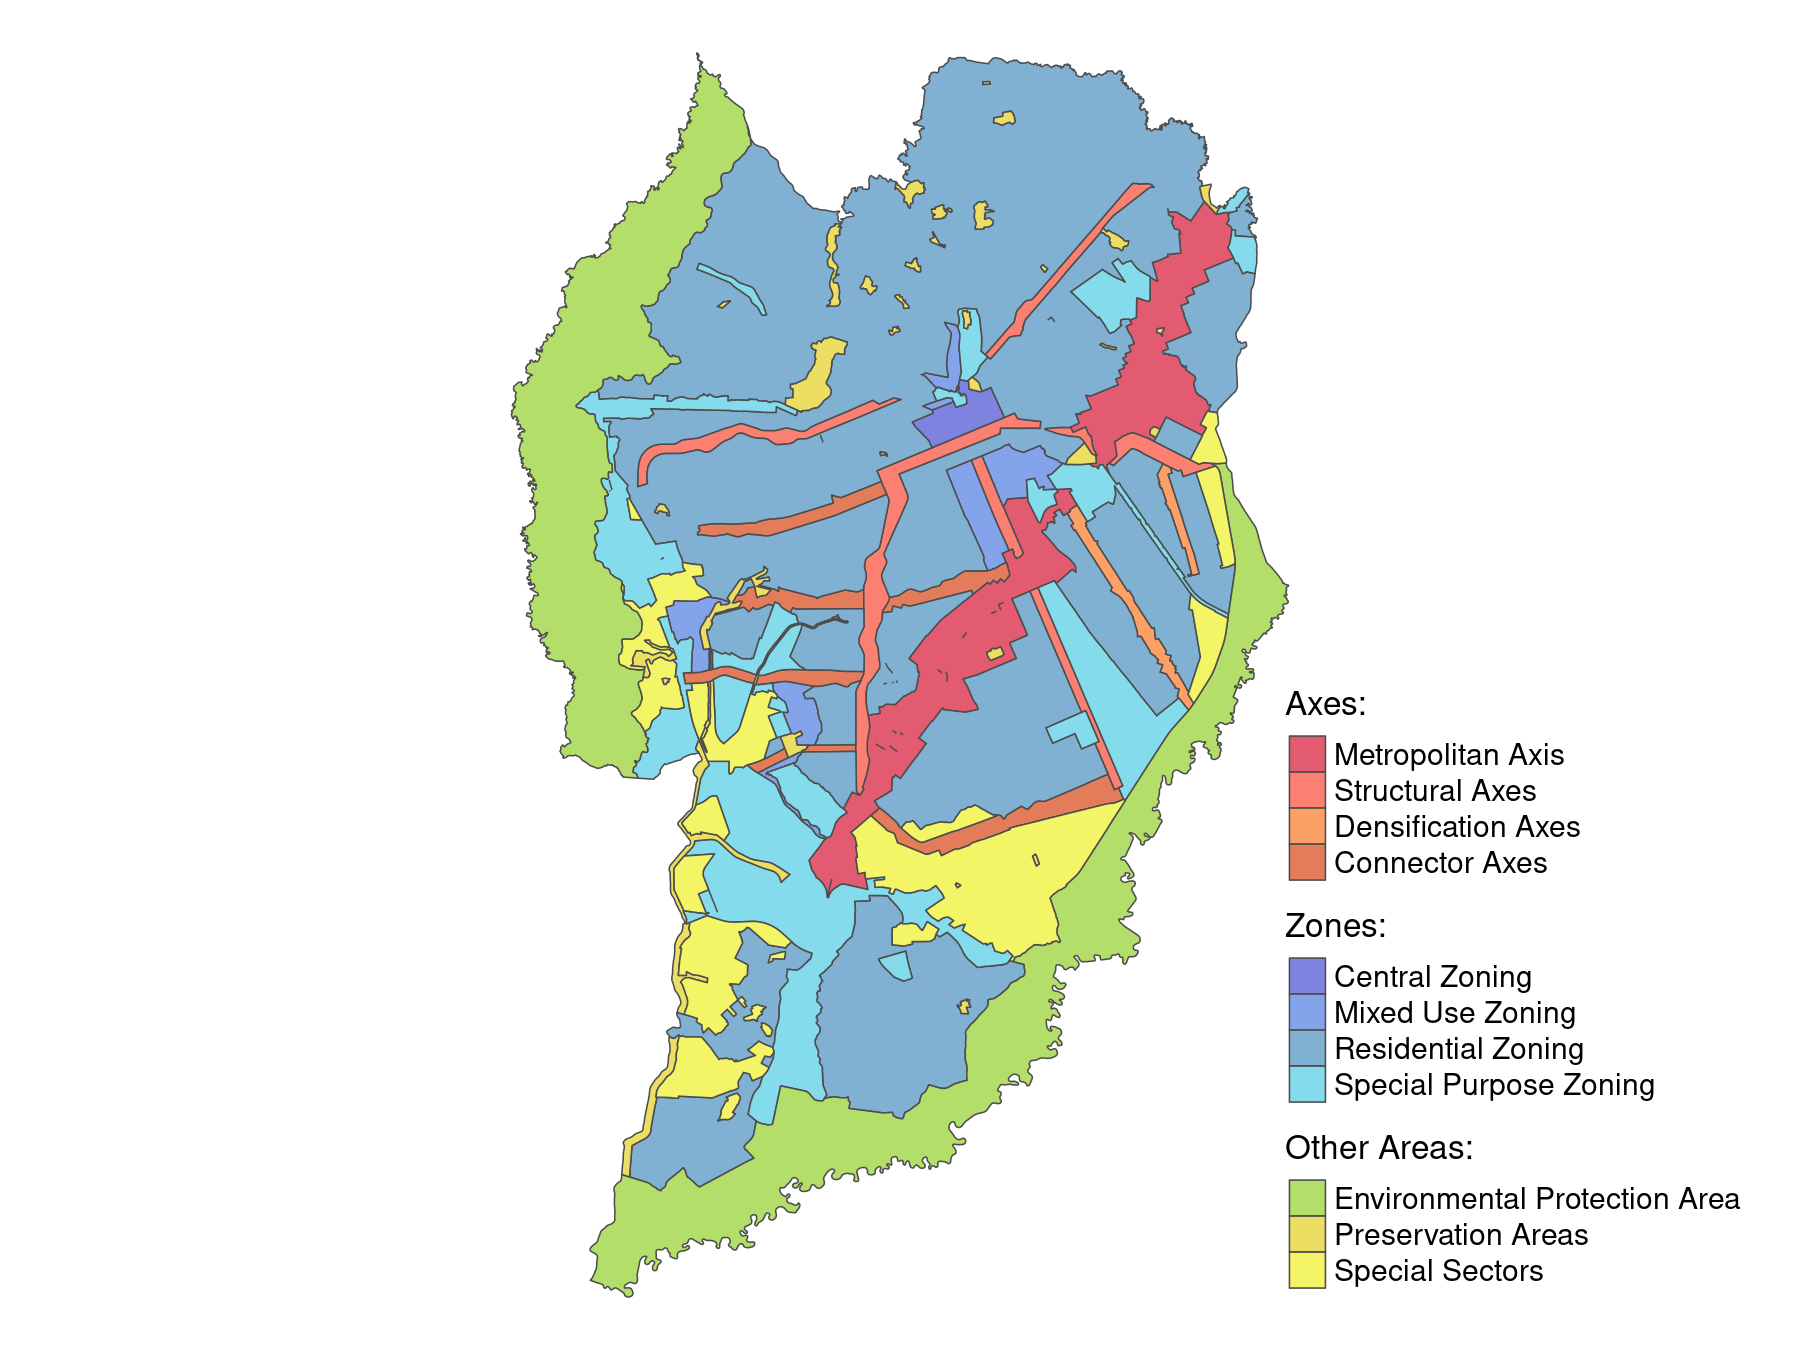
\includegraphics{fig/zoning_map.png}
    \label{fig:zoning}
    \par SOURCE: The Author (2022), based on \textcite{IPPUC2021}.
\end{figure}

%\begin{figure}[!htbp]
%    \centering\footnotesize
%    \captionsetup{font=footnotesize}
%    \caption{STRUCTURAL AXES IN CURITIBA}
%    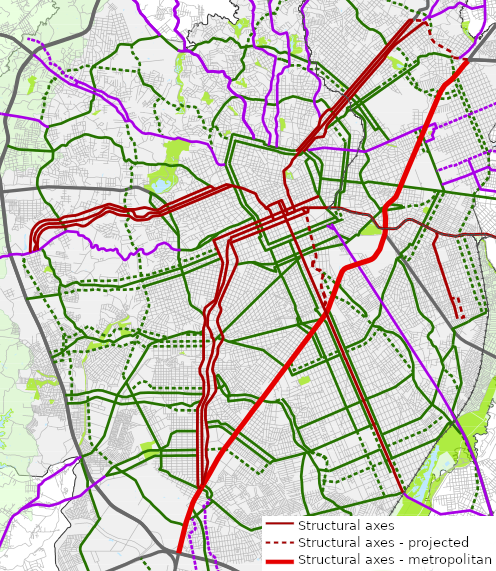
\includegraphics[width=0.6\textwidth]{fig/axes2.png}
%    \label{fig:axis}
%    \par SOURCE: Adapted from \textcite{Curitiba2015}.
%\end{figure}

Curitiba's land zoning plan splits the micro zoning system into four categories: central, residential, mixed use, and specific destination \cite{Curitiba2019a}. Central zoning involves the traditional downtown of the city, characterized by a high concentration of services, commerce, and jobs. Residential zones compass different types, depending on the density. It can include commercial units and a limited occupancy rate, depending on the environmental characteristics. Mixed use zones encourage the coexistence of residential and non-residential uses, mixing residences, services, and commercial units of medium density. Specific destination zoning can include educational, military, historic, and industrial uses, among others. Environmental protection areas have regulations that allow a safe level of occupation to the local environment. Preservation areas do not allow building occupation, in order to preserve bodies of water and its surroundings. Special sectors are areas destined to social housing projects, involving low and medium density residential zoning. 

Regarding the population density, \textcite{Curitiba2015} establishes a low density level as 80 residences per hectare, medium density between 80 and 200 residences per hectare, and high density between 200 and 400 residences per hectare. \autoref{fig:macro} shows how these higher densities are set in the metropolitan and structural axes. The areas in red represent the higher density zoning. Medium density zoning is established in the densification and connector axes. 

\begin{figure}[!htbp]
    \centering\footnotesize
    \captionsetup{font=footnotesize}
    \caption{LAND USE DENSITIES IN CURITIBA}
    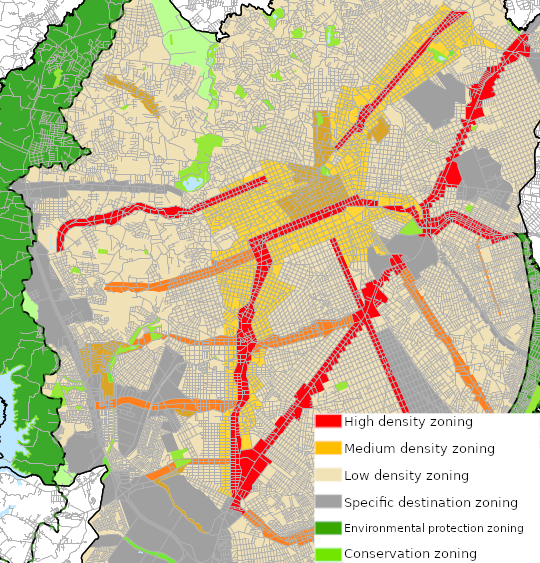
\includegraphics[width=0.6\textwidth]{fig/macro3.png}
    \label{fig:macro}
    \par SOURCE: Adapted from \textcite{Curitiba2015}.
\end{figure}

%% Road axis
Road hierarchy in Curitiba can be classified using the land zoning characteristics, defined by \textcite{Curitiba2019a}, and using the definition established by the Brazilian Traffic Code (\textit{Código de Trânsito Brasileiro - CTB}). In \autoref{fig:road_cwb}, a map with Curitiba road hierarchy, based on land zoning, is presented. Highways are high-speed roads that are administrated by state and federal governments. Structural roads are positioned inside the structural axes. They are arranged in a trinary system, which includes a dedicated bus lane among slow lanes in the center, and two parallel external one-way streets, destined for the continuous flow of vehicles. Sectorial roads have long extension and connects multiple regions of the city and it's neighbors, with a good integration to the structural system. Collector roads have medium to small extension and are designed to handle local traffic. Prioritized roads are located close to the city center. They are designed to handle a great volume and flow of traffic. The ``other'' category are streets that are not directly characterized in Curitiba's land zoning \cite{Curitiba2019a}. 

\begin{figure}[!htbp]
    \centering\footnotesize
    \captionsetup{font=footnotesize}
    \caption{ROAD HIERARCHY IN CURITIBA (LAND ZONING)}
    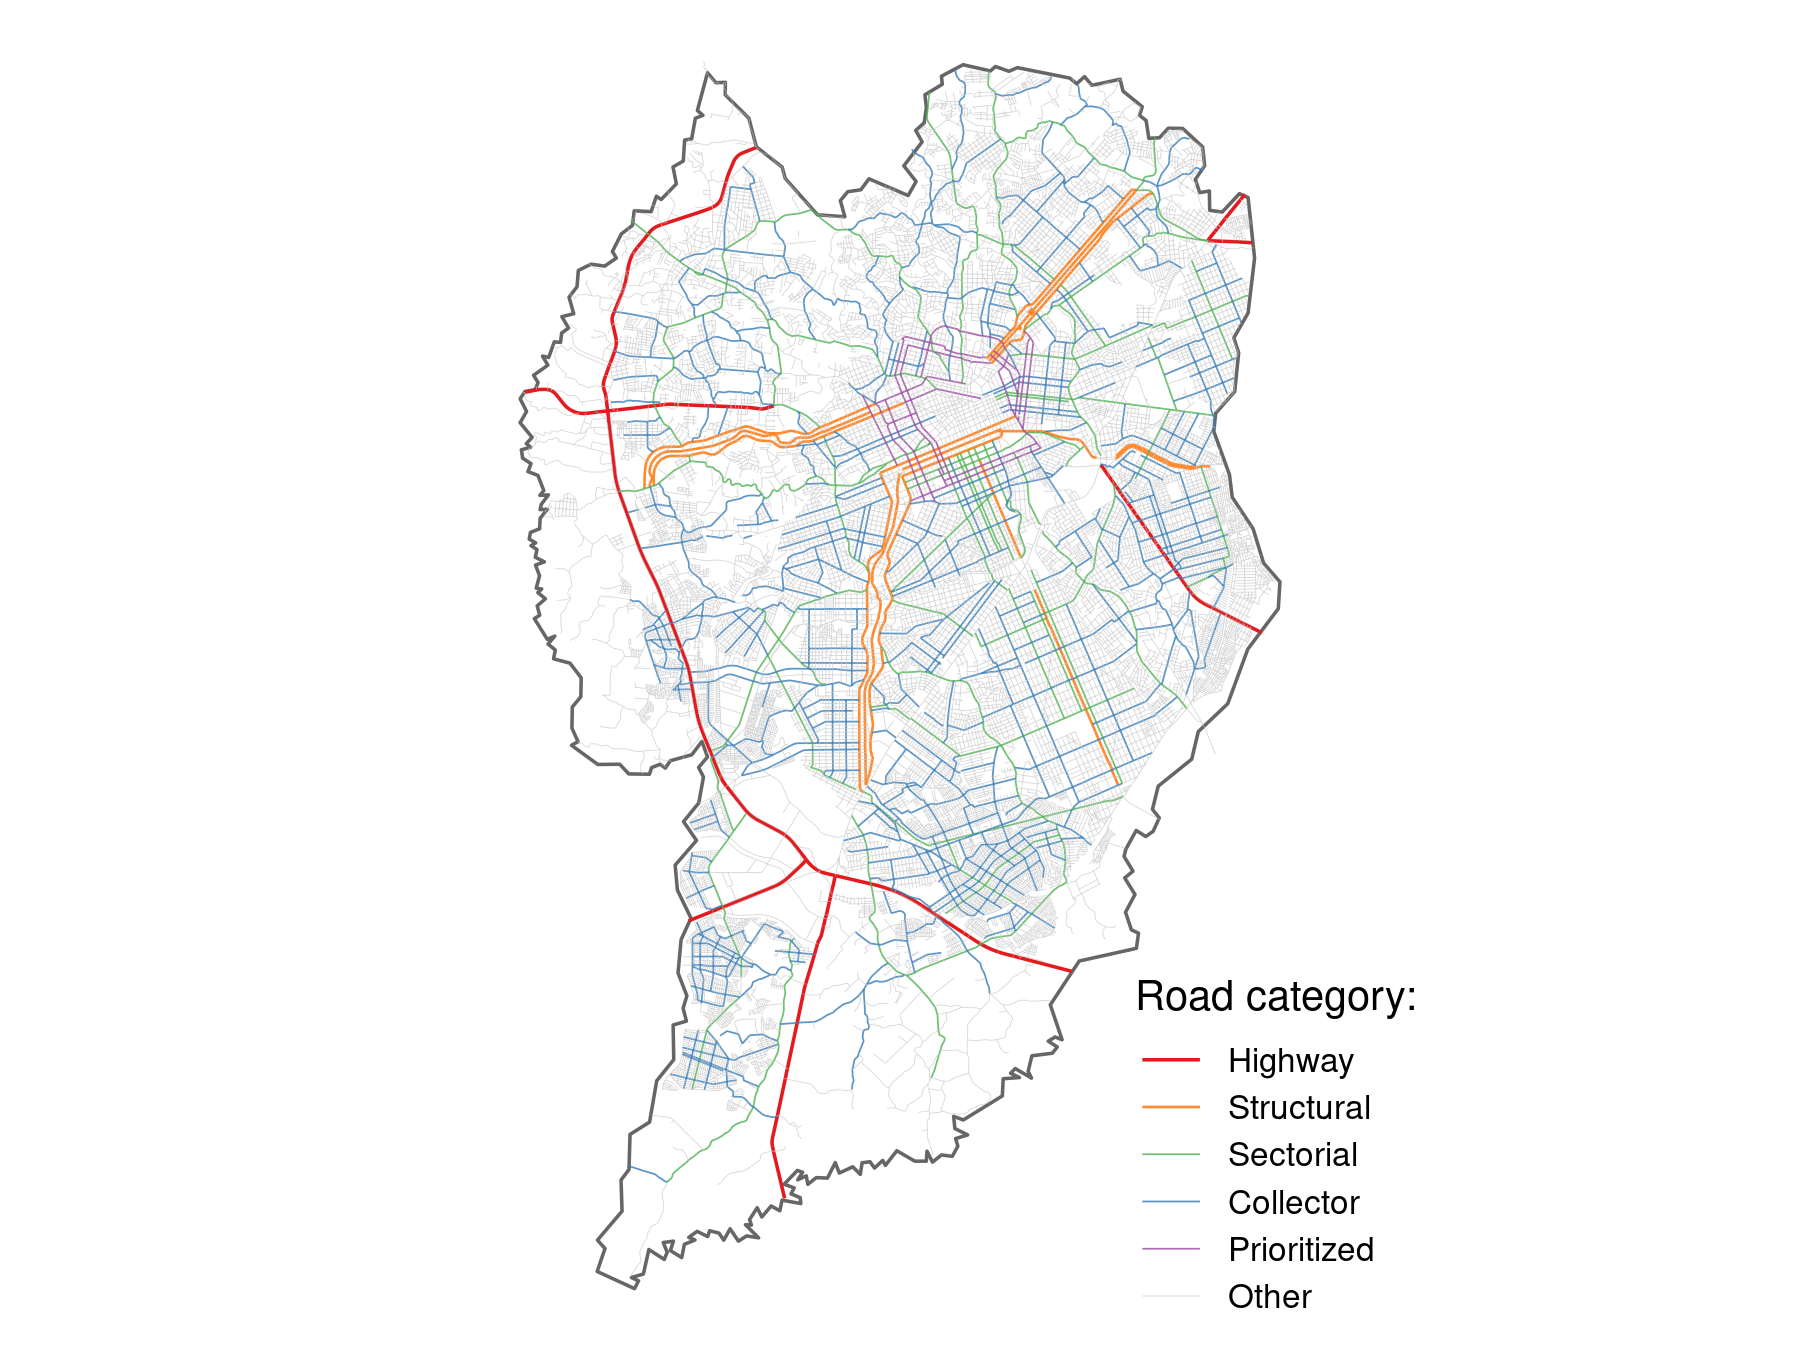
\includegraphics{fig/road_zoning_map.png}
    \label{fig:road_cwb}
    \par SOURCE: The Author (2022), based on \textcite{IPPUC2021}.
\end{figure}

In \autoref{fig:road_ctb}, the road hierarchy in Curitiba is presented, based on the CTB classification. Rapid transit roads are designed to handle a high flow of vehicles in higher speeds. Arterial roads are designed to handle a high amount of traffic flow and volume, while still offering a certain level of access to lots. Collector roads handle local traffic and connects local roads to main arterial and rapid transit roads. Local road's main function is to offer local access to neighboring lots \cite{Brasil1997}. 

\begin{figure}[!htbp]
    \centering\footnotesize
    \captionsetup{font=footnotesize}
    \caption{ROAD HIERARCHY IN CURITIBA (CTB)}
    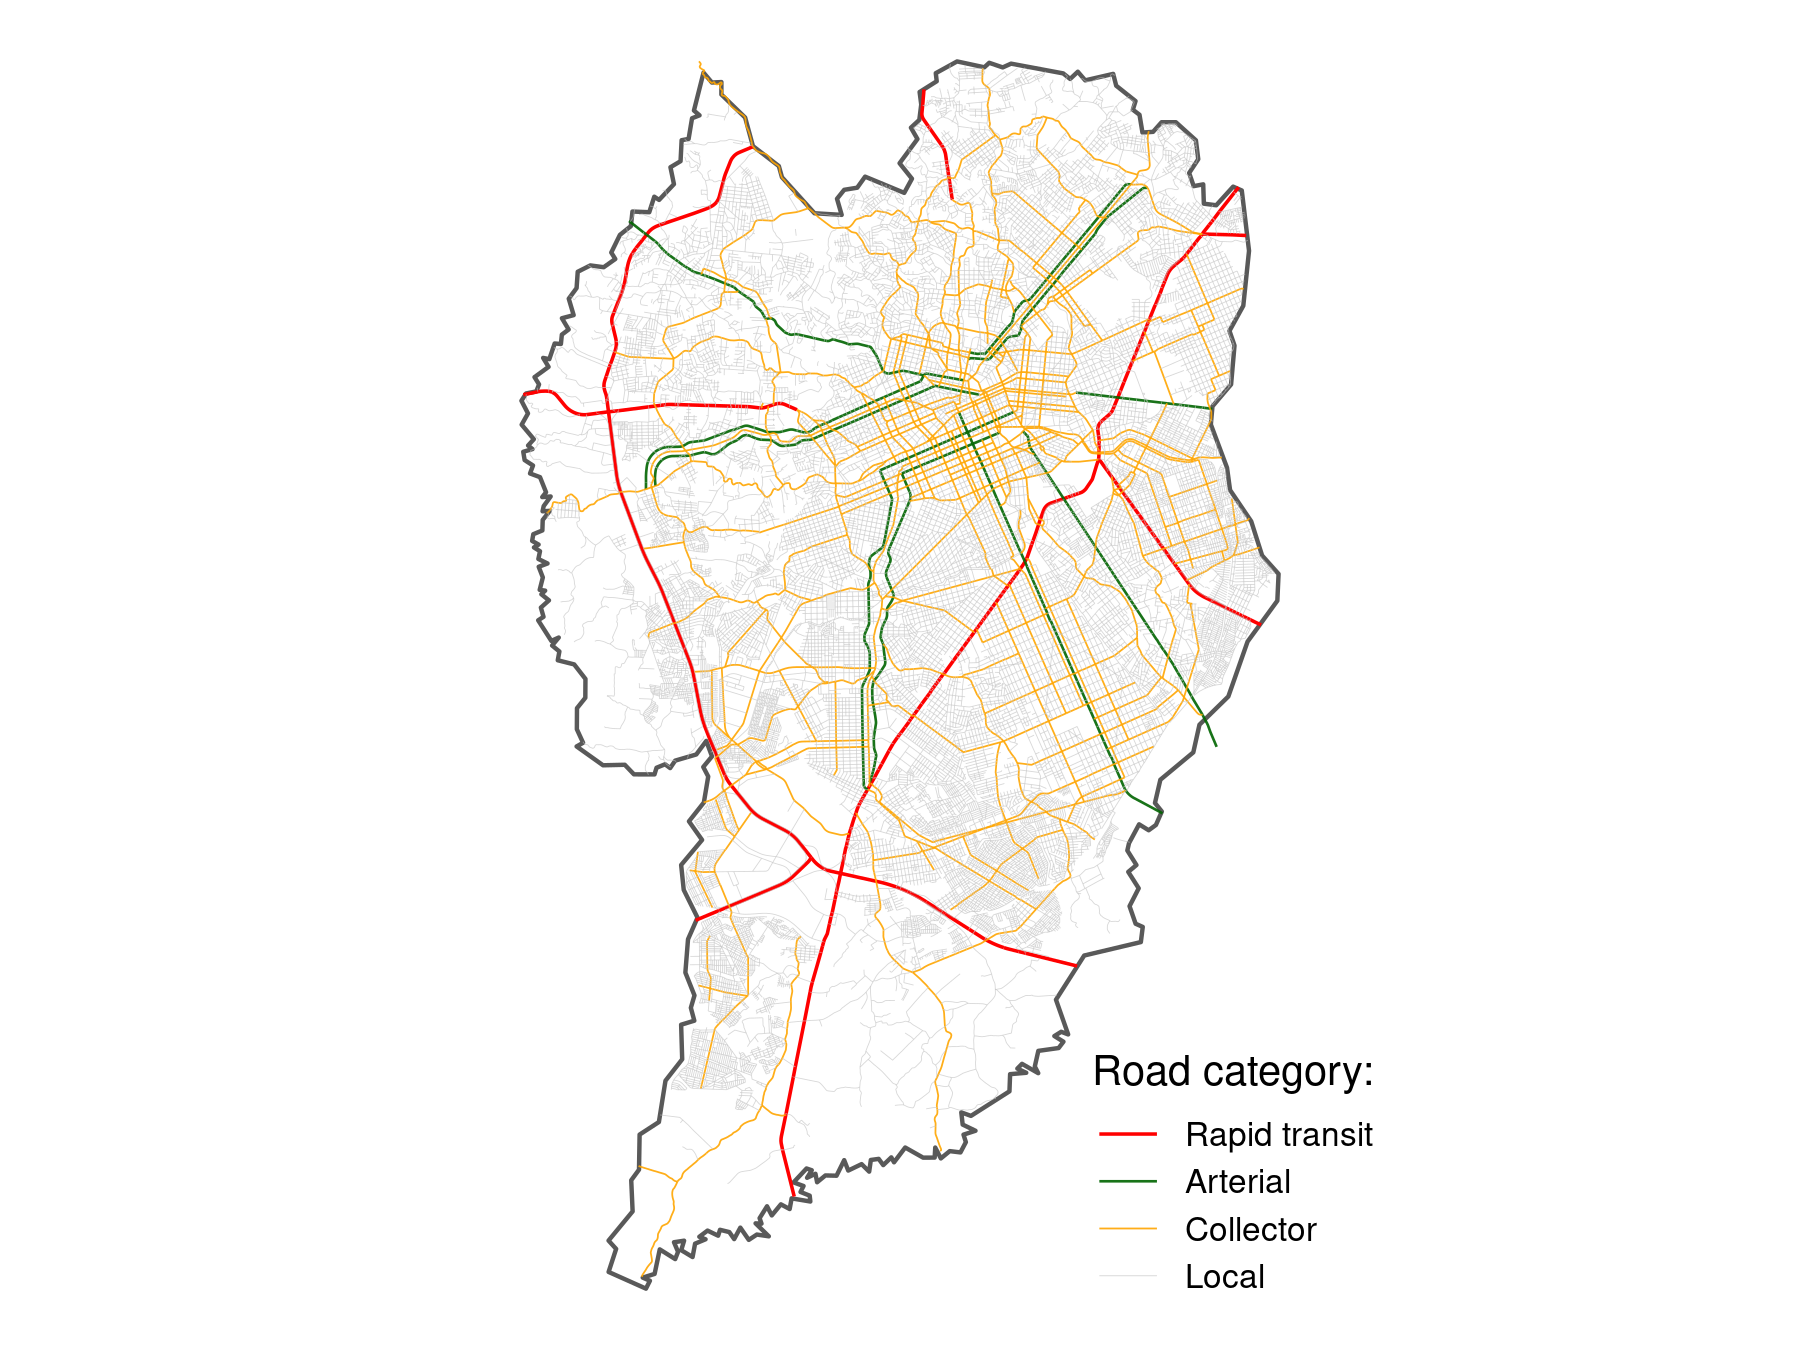
\includegraphics{fig/road_cwb_map.png}
    \label{fig:road_ctb}
    \par SOURCE: The Author (2022), based on \textcite{IPPUC2021}.
\end{figure}

%%

From decades ago until today, the majority of the urban environment was built for and around the needs of car users. Building and land use codes impact road traffic accident rates, including speeding as a major risk factor \cite{Knoflacher2016}. Urban planners and decision-makers need to recognize and understand the traffic safety impacts generated by planning policy and practice, as well as the benefits of creating new spaces and land patterns that favor adequate road safety levels for all users. 

\section{NATURALISTIC DRIVING STUDIES} \label{nds}

Human behavior research with a focus on road traffic safety might be performed applying multiple methods, including digital simulations, driving simulators, and on-the-road studies. Digital simulations studies consist of modeling a hypothetical situation based on statistical and microsimulation functions, which can be run multiple times in software. Driving simulation studies contain a physical mockup of a real vehicle, where the subject drives on the computer-generated scenario. On-the-road studies consist of using scenarios with real road users and can be categorized into two types: experimental and observational studies \cite{Shinar2017}. 

\begin{figure}[!htbp]
    \centering\footnotesize
    \captionsetup{font=footnotesize}
    \caption{BEHAVIORAL TRAFFIC SAFETY STUDIES}
    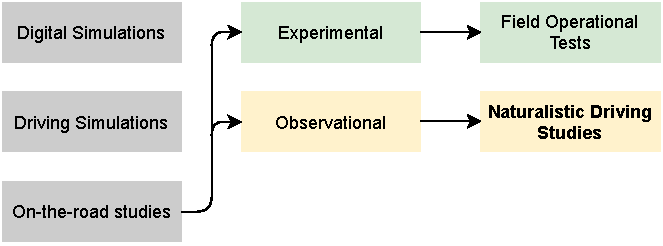
\includegraphics{fig/studies.pdf}
    \label{fig:shinar}
    \par SOURCE: The Author (2022), based on \textcite{Shinar2017}.
\end{figure}

Experimental studies contain some level of manipulation or control of the situation, where the independent variable is manipulated. This allows to better analyze the involved variables individually, but creates an artificial scenario, different from everyday situations. One popular type of experimental method is the field operational test (FOT). In FOT, volunteers are provided with cars equipped with multiple unobtrusive sensors, to investigate how they react to a specific system installed by the researchers. Diversely, in observational studies, researchers simply observe the behavior of drivers in natural conditions, without the control of dependent and independent variables \cite{Shinar2017}. 

A type of observational study is the naturalistic driving study (NDS). NDS consists of monitoring drivers' behavior in their cars, both in normal and safety-critical conditions. Participants' cars are usually equipped with video cameras, GPS systems and other sensors. The objective of the NDS is to record the driver's behavior during an everyday scenario. The cameras allow the recording of the driver, the car panel, instruments, and the recording of the surrounding areas, including other vehicles, pedestrians, and environmental elements. GPS or similar equipment allow the registration of the driver's instant speed and position \cite{Shinar2017}. Therefore, NDS is a method that can collect information about the environment, the vehicle, and human behavior.

The main difference between FOT and NDS is the element of study. FOT's usual objective is to evaluate a particular system or instrument inside or outside the vehicle. NDS' main objective is to record typical driving behaviors in multiple situations, including situations that present a risk for the occurrence of road traffic crashes, like speeding behavior and use of mobile phones, for example. NDS generates big data sets in comparison to other methods like FOT or driving simulators, but the method has its disadvantages as well. 

In the field of behavioral studies, NDS could be considered as an ``improvement'' in comparison to driving simulation studies. Its advantages and disadvantages make NDS a complementary method, not a competitive one. In a driving simulation, the sample size is smaller, and the immersion is not perfect, given the possibility of the occurrence of motion sickness and adaptation period of the participants. However, the main strength of driving simulators is the fact that it is possible to create and control events and stimuli in the scenario, enabling researchers to better isolate variables and replicate crashes, near-crashes, and critical events \cite{Shinar2017}.   

In comparison, NDS has a typically large sample size and provides practically total immersion in the participants' everyday trips. The events that occurred in traffic are uncontrolled and real. This gives a higher ``credibility'' to the collected data, but makes it harder to isolate the desired variables under investigation. The exposure to the experiment is usually higher in NDS, given that the participants have the data registered over multiple trips \cite{Carsten2013}. In general, the NDS characteristics and advantages are valuable to the present study, considering its capability of collecting a comparably large dataset of speeds and locations throughout the city's territory. In other words, instant speed data from real drivers spread into a real driving scenario is a desirable basis for understanding the influence of the built environment on speed choice behavior.

\autoref{tab:nds} contains some main NDS researches performed in the last two decades. The 100-Car Naturalistic Driving Study, conducted by the Virginia Tech Transportation Institute (VTTI), was the first-large scale NDS, and it was performed in the United States. Its instrumentation was composed of 5 cameras, 1 accelerometer and 1 GPS sensor, among other monitoring devices. Some vehicles were owned by the researchers and others by the participants. The main location of the study was the metropolitan area of Northern Virginia and Washington, D.C. The main goal of the research was to maximize the potential to record crash and near-crash events. In total, 100 vehicles were used, including 241 participants. The total trip time of the data collected was above 40,000 hours, with a distance above 3 million kilometers \cite{Neale2005}.

\begin{table}[!hbtp]
    \footnotesize
    \captionsetup{justification=raggedright,
        singlelinecheck=false,
        font=footnotesize}
    \caption{NATURALISTIC DRIVING STUDIES PROGRAMS}
    \centering
    \begin{tabular}{llllll}
        \hline
        \multicolumn{1}{c}{\textbf{Program}} & \multicolumn{1}{c}{\textbf{Countries}} & \multicolumn{1}{c}{\textbf{Vehicles}} & \multicolumn{1}{c}{\textbf{Drivers}} & \multicolumn{1}{c}{\textbf{Hours}} & \multicolumn{1}{c}{\textbf{Distance} $[km]$} \\
        \hline
        100 Car NDS & USA        & 100 & 241 & 42,300 & 3,218,688 \\
        SHRP2 NDS   & USA        & 3,500$^{(2)}$ & 3,500$^{(2)}$ & 1,000,000$^{(2)}$ & 56,327,040 \\
        ANDS        & Australia  & 346 & 409 & 716,320 & 1,512,630 \\
        UDRIVE      & EU$^{(1)}$ & 287 & 287 & 87,870 & 4,000,000$^{(2)}$ \\
        CNDS        & Canada     & 140 & 149 & 53,000$^{(2)}$ & 1,800,000$^{(2)}$ \\
        Candrive I  & Canada     & 100 & 100 & - & - \\
        -           & Japan      & 60  & 60  & - & - \\
        SH-NDS      & China      & 5   & 60  & - & 161,055 \\
        -           & Iran       & 52  & 52  & 546$^{(2)}$ & 25,740$^{(2)}$ \\
        NDS-BR      & Brazil     & 32  & 32  & 381 & 9,444 \\ 
        \hline
    \end{tabular}
    \label{tab:nds}
    \par \vspace{2mm} \footnotesize \raggedright
    SOURCE: The Author (2022).
    \par \vspace{1mm} \footnotesize \raggedright
    NOTES: $^{(1)}$: United Kingdom, Netherlands, France, Spain, Germany, and Poland; $^{(2)}$: Approximate values.
\end{table}

Another NDS study performed in the United States was the SHRP2 (Strategic Highway Research Program-2) NDS, gathering a massive quantity of data. The study was conducted in 6 states, with more than 3,500 vehicles, one million hours of video and trip data collected and 56 million kilometers traveled. More than 1,500 crashes were registered, establishing a valuable sample for road safety studies \cite{Njord2015}. The Australian Naturalistic Driving Study (ANDS) launched in 2015, aiming to collect road safety data from 360 vehicles – 180 in Sydney and 180 in Melbourne. Vehicles are equipped with 4 cameras, GPS sensors, and an accelerometer \cite{ANDS2017a}. According to \textcite{Larue2019}, the ANDS was able to collect data from 346 vehicles and 409 participants. The last report related a collection of more than 700,000 hours of traveled period and more than 1,500,000 kilometers of traveled distance \cite{ANDS2017a}. 

In the European Union, the UDRIVE naturalistic driving study was a large-scale program performed in 6 EU countries: United Kingdom (UK), the Netherlands, France, Spain, Germany, and Poland. It lasted for 5 years, between 2012 and 2017, and its objective was to collect behavioral data from three transportation modes: cars, trucks, and powered two-wheelers. Two hundred eighty-seven vehicles and drivers were part of the research. The data collected reached almost 90,000 hours of driving data and approximately 4,000,000 kilometers of traveled distance \cite{VanNes2019}. The Canadian Naturalistic Driving Study (CNDS) instrumented a total of 140 vehicles, including cars, pickup trucks, and minivans, with 4 cameras, a frontal radar sensor, and one GPS radar. One hundred forty-nine drivers participated in the study, with approximately 53,000 hours of data collected and 1,800,000 kilometers of traveled distance \cite{CNDS2021}. Also in Canada, the first phase of the Canadian Safe Driving Study (Candrive I) had the participation of 100 active drivers, with age equal to or above 70 years old. The main objective of this NDS was to investigate the fitness to drive of older drivers \cite{Marshall2013}. 

%% Japan, China and Iran

In Japan, an NDS was conducted between 2006 and 2008, with the participation of 60 drivers and vehicles. The study was conducted in 16 different regions in Japan. The DAS utilized in the study contained a GPS sensor, 5 cameras, an accelerometer, a steering sensor, and digital switches to detect the use of brake and turn signals \cite{Uchida2010}. The Shanghai Naturalistic Driving Study (SH-NDS) was conducted between 2012 and 2015 in Shanghai, China. The study contained 60 participants, who drove 161,055 kilometers. Five vehicles equipped with a DAS developed by VTTI were used in this research \cite{Zhu2018}. Also in Asia, an NDS was conducted in Iran, between April 2017 and April 2018. The study had the participation of 52 drivers, with a pair of cameras equipped in their vehicles. The cameras allowed the recording of conflict events between motorized vehicles and pedestrians in marked ($n = 392$) and unmarked ($n = 956$) crosswalks \cite{Sheykhfard2021}. The sample contained approximately 546 hours of data collected and 25,740 kilometers of traveled distance.

In Brazil, a naturalistic driving study was established in 2019 in the city of Curitiba-PR, conducted by the Universidade Federal do Paraná, funded by the National Council for Scientific and Technological Development (CNPq) and by the National Observatory for Road Safety. A group of partner universities also participate in the project. The Naturalistic Driving Study – Brazil (NDS-BR) has already collected data from 16 instrumented vehicles, each with a set of 3 cameras and 1 GPS sensor. Currently, NDS-BR collected almost 382 hours of driven time and 9,444 km of traveled distance in Curitiba and the metropolitan area. This research is still ongoing, and further details about the process of data collection are discussed in Section \ref{ndsc}.

NDS allows the investigation of speeding episodes and how other factors can influence the occurrence of speeding. These factors can include environmental elements (road infrastructure, built environment, weather, traffic conditions, etc.), human and behavior elements (age, gender, secondary tasks engagement, education, personality),  and vehicle characteristics (engine power, level of conservation). \textcite{Richard2013,Richard2017, Richard2020} used NDS speed data to better understand different types of speeding and how the drivers behave towards them. \textcite{Richard2013} established a classification called behavioral speeding, splitting it into 4 types. The first type consists of speed below the posted limit. In the second type, drivers are speeding, but they feel like they are driving at a safe speed. On the third type, speed is above the enforcement limit, and the driver starts to accept a higher level of risk. The 4th type consists of reckless speeding, where the driver reaches speeds way above the speed limit, without any consideration to the risks. 

\textcite{Richard2017} clustered speeding behavior into 6 categories, from NDS data collected from 88 drivers in Seattle. The authors used the k-means method on the sample, resulting in 6 clusters: (i) speeding up, (ii) speed drop, (iii) incidental speed, (iv) casual speeding, (v) cruising speeding, and (vi) aggressive speeding. Speeding up behavior consists of reaching a high exceeding speed in a short period, with high variability. Speed drop is complementary to speeding up, representing characteristics that are consistent with a braking behavior when entering a lower speed limit zone. 

Incidental speeding was the most common speeding type detected in the sample. It consisted of mean speeds barely above the speed limit, occurring in longer periods. Casual speeding was the second most common type, and it had similar behavior to incidental speeding, but it had a higher level of mean speed above the speed limit, with similar lengths of occurrence. Cruising speeding was a deliberate type of speeding, most common on freeways and state highways – places with more opportunity for speeding. Aggressive speeding presented higher levels of mean speed, with high variability in longer periods. In this cluster, drivers engaged in repeated speed adjustments, always trying to reach maximum speed.

\textcite{Richard2020} used a sample of 100 trips from the SHRP2 NDS database to examine how the occurrence of speeding episodes is affected by basic factors. The authors found drivers in the age group between 16 and 24 had more speeding episodes than other age categories. Considering the days of the week, the occurrence of speeding was lower between Monday and Thursday. Highways present higher free-flow and speeding episodes in comparison to other types of roads. 

\textcite{Ellison2015} analyzed speeding data from 106 drivers in Sydney, collected with the use of NDS, to establish how much time drivers are saving with speeding in urban environments. The speeding stretch of a trip was compared to a simulated stretch with the speed limit traveling the same length. Then, the time delta between the two scenarios was calculated to create the time saved during the speeding episode. The results showed an average time saving of 26 seconds per day or 3 minutes per week. Considering the median driver, less than 2 hours per year is saved, and 75\% of drivers never save more than 3 min in a single day. 

\textcite{Hamzeie2017} investigated how the average speed chosen by drivers was influenced by the traffic conditions and how it affected the risk of crashes. The authors used the SHRP2 NDS data and concluded that higher travel speeds were directly correlated to higher speed limits, and high speed variance is correlated to a higher risk of a crash. \textcite{Kong2020} also investigated speeding behavior patterns related to the traffic and road conditions, from a sample of naturalistic data collected from 92 vehicles. The authors concluded that speeding duration is related to driving on roadways with higher function classes, to longer trips, and to speed loss caused by congestion, causing the\ idea of needing to ``recover the lost time'' by the drivers.

Using the NDS-BR data, \textcite{Bastos2021} compared risky behavior between carpooling and non-carpooling drivers, including speeding. The authors concluded that carpooling drivers presented a safer behavior towards speeding, having fewer episodes in comparison to non-carpooling drivers. \textcite{Bastos2020a} also investigated the occurrence of mobile phone use (MPU) while driving and concluded that MPU occurs in higher frequencies when the average speed is lower. To analyze the relationship between speeding and speed cameras, \textcite{Amancio2021} also used the NDS-BR dataset to investigate the effect of speed cameras on the average speeds of vehicles on arterial roads. The author concluded an average speed reduction before and near the cameras, and an increase after passing through the speed cameras. Considering other physical elements of the road network, \textcite{suguinoshitaFATORESDETERMINANTESPARA2020} investigated elements of arterial roads and its effects on average speeds, and \textcite{szeligaIMPACTOCURVASHORIZONTAIS2020,szeligaAnaliseVelocidadePraticada2021} investigated the effects of horizontal curves and conversion maneuvers on the practiced speeds of drivers.
% Insert Suguinoshita, Szeliga and Szeliga. 

With the use of the SHRP2 NDS database, \textcite{Dingus2016} investigated 905 crash events, relating them to the behavior of the drivers. The authors focused on four behavioral categories: observable impairment; driver performance error; driver judgment error; and observable driver distraction. Speeding behavior was considered a judgment error. Results include that speeding behavior increases crash risk 12.8 times more than the ``model driving episodes'' (without speeding). Overall, the papers cited in this section are just a small sample of the existing studies including speeding behavior and NDS data. In the scope of the NDS projects that were concluded or are ongoing, there is a comprehensive database of speed and speeding episodes, making it possible to continuously investigate this risk behavior. 

\section{GEOGRAPHICALLY WEIGHTED REGRESSION} \label{sec:gwr}

Regression analysis is a tool to investigate the dependency between variables and to predict future parameters based on previous ones. This type of statistical analysis can show the relationship between dependent variables \cite{Lindley1987}. In the investigation of the effects of the built environment on the occurrence of crashes in urban areas, negative binomial (NB) regression is a traditional model used \cite{Wei2013, Zhang2014}. However, the quality of this model is limited by the incapacity of analyzing the spatial dependency and heterogeneity expected to happen on road safety factors related to the urban environment \cite{Obelheiro2019}.

% Explain better why GWR is batter and how the previous studies are less precise. 

To overcome this limitation, the Geographically Weighted Regression (GWR) allows the exploration of the relationship between variables in a spatial nonstationarity context. The spatial nonstationarity context consists of a scenario where it is assumed that parameters are not constant across the space. A global regression model may be incapable of explaining the relationship between a set of variables with an acceptable level of precision in this scenario. The GWR model considers that the nature of the model must alter over space to reflect the structure within the data, allowing the actual parameters for each location in space to be modeled and mapped \cite{Brunsdon2010}.

The basic form of GWR is detailed on the following equation:\begin{align}
    y_i = \beta_{i0} + \sum_{k=1}^{m} \beta_{ik} x_{ik} + \epsilon_i \mbox{;}
    \label{eq:gwr}
\end{align} where $y_i$ is the dependent variable at location $i$, $x_{ik}$ is the value of the $k$th independent variable at location $i$, $m$ is the number of independent variables, $\beta_{i0}$ is the intercept parameter at location $i$, $\beta_{ik}$ is the local regression coefficient for the $k$th parameter at location $i$, and $\epsilon_i$ is the random error at location $i$. The GWR model depends on a spatial weighting function called $w_{ij}$ that controls the contribution of point $j$ on the calibration of a model for point $i$. The spatial weighting function represents the idea that for each point, $i$ there is a bump of influence around it. Considering this ``bump'', observations closer to $i$ have more influence in the estimation of $i$'s parameters \cite{Brunsdon2010,Gollini2013}.

In the context of a multivariate GW model, these influences are calculated by a weighted least squares approach, described in the following equation: \begin{align}
    \hat{\beta}_i = \left(X^TW\left(u_i,v_i\right)X\right)^{-1}X^TW\left(u_i, v_i \right)y\mbox{ ;}
    \label{eq:wls}
\end{align} where $X$ is the matrix of the independent variables with a column of 1s (ones) for the intercept, $y$ is the dependent variable vector, $\hat{\beta} = \left(\beta_{i0},...,\beta_{im}\right)^T$ is the vector of $m + 1$ local regression coefficients and $W_i$ is the diagonal matrix denoting the spatial weighting ($w_{ij}$) of each observed data for regression point $i$ at location $(u_i, v_i)$ (defined by the selected spatial weighting function) \cite{Gollini2013}. The spatial weighting function is also known as the kernel function. This function can have multiple configurations, including Gaussian, Exponential, Boxcar, Bisquare, and Tricube configurations, as detailed in \autoref{tab:kernel}.

\begin{table}[!hbtp]
    \footnotesize
    \captionsetup{justification=raggedright,
        singlelinecheck=false,
        font=footnotesize}
    \caption{KERNEL FUNCTIONS}
    \centering
    \begin{tabular}{ll}
        \hline
        \multicolumn{1}{c}{\textbf{Kernel}} & \multicolumn{1}{c}{\textbf{Equation}}  \\
        \hline
        Global Model             & $w_{ij} = 1$                              \\
        Gaussian \rule{0pt}{3ex} & $w_{ij} = \exp \left(- \frac{1}{2} \left(\frac{d_{ij}}{b}\right)^2\right)$ \\
        Exponential  \rule{0pt}{4ex} & $w_{ij} = \exp \left(- \frac{|d_{ij}|}{b}\right)$               \\
        Boxcar \rule{0pt}{4ex} & $w_{ij} = \begin{cases}
            1 & \mbox{if } |d_{ij}| < b, \\
            0 & \mbox{otherwise}
                                 \end{cases}$                               \\
        Bisquare \rule{0pt}{4ex} & $w_{ij} = \begin{cases}
            \left(1 - \left(d_{ij}/b\right)^2\right)^2 & \mbox{if } |d_{ij}| < b, \\
            0 & \mbox{otherwise}
                                 \end{cases}$                               \\
        Tricube \rule{0pt}{4ex} & $w_{ij} = \begin{cases}
            \left(1 - \left(|d_{ij}|/b\right)^3\right)^3 & \mbox{if } |d_{ij}| < b, \\
            0 & \mbox{otherwise}
                                 \end{cases}$                               \\
        \hline
        \end{tabular}
    \label{tab:kernel}
    \par \vspace{2mm} \footnotesize \raggedright
    SOURCE: \textcite{Gollini2013}
\end{table}

The distance between observations $i$ and $j$ is defined by $d_{ij}$, inside a chosen $b$ bandwidth, which is the key controlling parameter in all kernel functions. \autoref{fig:kernel} presents the plot of the kernel functions, for a generic bandwidth $b = 1000$, where $w$ is the weight and $d$ is the distance between two observations. As the plot shows, the global kernel function represents a global linear regression, where all the variables are constant across the space. The bandwidth has two configurations: fixed or adaptive. Fixed bandwidth consists of an absolute value of distance, presenting better outcomes for uniform-sized zonal levels \cite{Huang2018}, including grids with equal areas. Adaptive bandwidth consists in choosing a fixed quantity of neighbors for each regression point $i$, with variable sizes. This configuration works better for zonal levels with irregular sizes, including traffic analysis zones (TAZ) and census blocks \cite{Yu2017}. The size of bandwidth can be chosen with the use of a cross-validation function or testing multiple values to reach a lower value of corrected Akaike information criterion ($AIC_c$). These processes will be better explored in Section \ref{gwm}.

\begin{figure}[!htbp]
    \centering\footnotesize
    \captionsetup{font=footnotesize}
    \caption{KERNEL FUNCTIONS PLOT}
    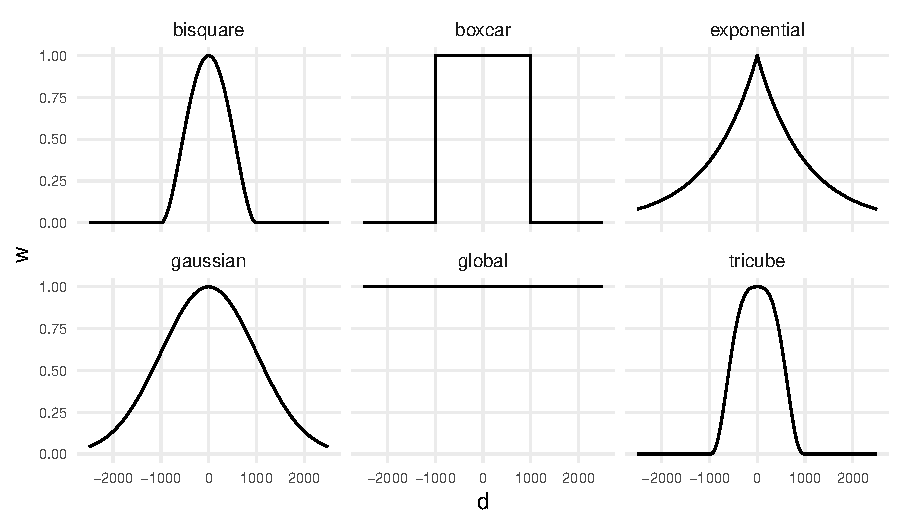
\includegraphics{fig/kernel.pdf}
    \label{fig:kernel}
    \par SOURCE: The Author (2022), based on \textcite{Gollini2013}.
\end{figure}

The GWR model presented in equation \ref{eq:gwr} has a limitation: it can be used only when the distribution of the dependent variable is Gaussian \cite{DaSilva2013a}. Therefore, count data needs other GWR configurations to fit in the model, including Poisson and Negative Binomial distributions. The Geographically Weighted Poisson Regression (GWPR) is described by \textcite{Obelheiro2020,Nakaya2005a} with the following equation: \begin{align}
    y_i \sim \mbox{ Poisson} \left[t_i \exp \left(\sum_k \beta_{ik} \left( u_{i}, v_{i} \right) x_{ik} \right) \right] \mbox{ ;}
\end{align} where $t_i$ is an offset variable and remaining variables are defined in equations \ref{eq:gwr} and \ref{eq:wls}. The Geographically Weighted Negative Binomial Regression (GWNBR) described by \textcite{DaSilva2013a} with the following equation: \begin{align}
    y_i \sim \mbox{ NB} \left[t_i \exp \left( \sum_k \beta_{ik} \left( u_{i}, v_{i} \right) x_{ik} \right), \alpha \left( u_{i}, v_{i}\right) \right] \mbox{ ;}
\end{align} where NB represents negative binomial and $\alpha$ is the parameter of over dispersion with spatial variation $\left(u_i, v_i\right)$. 

\autoref{tab:gwrworks} contains a set of studies in which GWR models were used to investigate the relationship between BE variables and road safety performance, measured by the occurrence of road crashes. Regarding the zonal level, most investigations used TAZ as the unit of analysis. \textcite{Obelheiro2020} created a traffic safety zonal level (TSAZ) based on census blocks. All authors but one used an area as zonal level. \textcite{Arvin2019} performed GWR models using intersection points as the location of regression. 

\begin{table}[!htbp]
    \footnotesize
    \captionsetup{justification=raggedright,
        singlelinecheck=false,
        font=footnotesize}
    \caption{GWR AND ROAD SAFETY STUDIES}
    \centering
    \begin{tabular}{lllp{1.6cm}l}
        \hline
        \multicolumn{1}{c}{\textbf{Author}} & \multicolumn{1}{c}{\textbf{Zonal level}} & \multicolumn{1}{c}{\textbf{Distribution}} & \multicolumn{1}{c}{\textbf{Kernel}} & \multicolumn{1}{c}{\textbf{Bandwidth}} \\
        \hline 
        \textcite{Amoh-Gyimah2017} & TAZ, grid & Poisson & Bisquare, gaussian & Adaptive \\
        \textcite{Arvin2019} & Intersections & Poisson & Bisquare, gaussian & Adaptive \\
        \textcite{Hadayeghi2010} & TAZ & Poisson & Bisquare, gaussian & - \\
        \textcite{Huang2018} & Census block & Gaussian & - & Fixed \\
        \textcite{Obelheiro2019} & TAZ & Poisson, NB & - & Adaptive \\
        \textcite{Obelheiro2020} & TSAZ & Poisson, NB & - & Adaptive \\
        \textcite{Pirdavani2014} & TAZ & Gaussian & Bisquare, gaussian & Adaptive \\
        \textcite{Rhee2016} & TAZ & Gaussian & Gaussian & Fixed \\
        \textcite{Yu2017} & Census block & NB & - & Adaptive \\
        \textcite{Zhang2015} & TAZ & Poisson & - & - \\
        \hline
    \end{tabular}
    \label{tab:gwrworks}
    \par \vspace{2mm} \footnotesize \raggedright
    SOURCE: The Author (2022)
\end{table}

Regarding the type of GW model, most authors chose GWNBR or GWPR, considering that road crash count distribution fits better in these models. Concerning kernel type, it only varied between two options: Bisquare and Gaussian. Most studies contained the use of adaptive kernels, which is a better option for zonal levels with irregular sizes. In conclusion, GWR is a method that enables the exploration of findings that might otherwise be missed if only a global regression method is applied. It is always important to check if the GWR model better describes the data than a global regression model, comparing the results from both. All the processes of constructing a GWR model and its parameters for this work are described in Section \ref{gwm}.

%-------------------------------------------------------------------------------

\chapter{METHODS} \label{cap:methods}

This chapter is divided into 4 sections. Section \ref{ndsc} contains the steps of collecting and processing naturalistic driving data. Section \ref{data} presents the process of creating the dependent and independent variables. Section \ref{gwm} includes the process of elaborating a GWR model. Section \ref{sec:cluster} contains the process of calculating a local indicator of spatial association (LISA) using the Local Moran statistic to identify spatial clusters in the GWR results and desired variables. All process described in Sections \ref{data} through \ref{sec:cluster} were executed using the R programming language \cite{rcoreteam2021}. The code can be accessed at \textcite{santos2022}.  
 
\section{NATURALISTIC DATA COLLECTION} \label{ndsc}

%% How data was collected, where it was collected, from who it as collected, when it was collected

%% Ref Jackson: gps2csv.py; functions.py; video.py ... (appendix)

% 1. Equipment: composition and how it was installed (equip. scheme - borguezani, camera scheme - amancio)

The Naturalistic Driving Study – Brazil (NDS-BR) utilized non-intrusive instrumentation of vehicles, with two data acquisition systems (DAS). Each DAS contained three high-definition cameras, one GPS sensor, one laptop with a GNU/Linux operating system distribution, and one power supply. One camera was positioned on the right window of the car, towards the inside of the vehicle, facing the driver. Two other cameras were positioned on the windshield of the car, facing towards the front outside. Considering these two, one camera was facing slightly to the left and another one to the right. The visual scheme of camera positioning is presented in \autoref{fig:cam_install}.

\begin{figure}[!htbp]
    \centering\footnotesize
    \captionsetup{font=footnotesize}
    \caption{CAMERA POSITIONING INSIDE THE VEHICLE}
    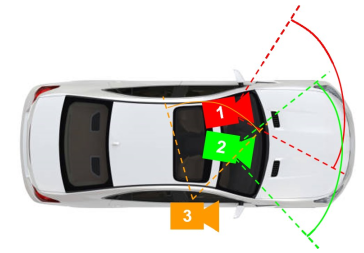
\includegraphics[width=0.6\textwidth]{fig/cam_install.png}
    \label{fig:cam_install}
    \par SOURCE: \textcite{Amancio2021}.
\end{figure}

The GPS sensor was positioned near the car panel. The cameras and GPS sensor were connected to the laptop, which controlled and synchronized the data acquisition. The laptop was installed inside a box, positioned on the floor by the passenger's seat. The DAS was installed in the private vehicle of each participant. There was no audio recording from inside the vehicle, to not inhibit possible conversation of the driver during the study. Cameras 1 and 2 enabled the recording of visual data about the environment outside the vehicle – traffic conditions, traffic control, weather, conflicts with other vehicles, etc. Camera 3 allowed the collection of visual data about the behavior of the driver, including the use of seatbelt, mobile phone use, etc. \autoref{fig:cam_cap} contains images collected by the cameras.  

\begin{figure}[!htbp]
    \centering\footnotesize
    \captionsetup{font=footnotesize}
    \caption{CAMERA IMAGES}
    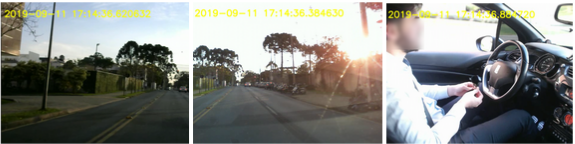
\includegraphics[width=0.9\textwidth]{fig/cam_cap.png}
    \label{fig:cam_cap}
    \par SOURCE: The Author (2022).
\end{figure}

% 2. Data processing: how they were processed (.py scripts), transformed to csv (gps2csv.py), valid time

The DAS allowed the acquisition of GPS and video data in synchronization, collecting information in a frequency of one second. The process of acquisition is illustrated in \autoref{fig:das}. The main controller of the data collection was the laptop. At the beginning of each trip, the driver needed to manually turn on the laptop after starting the car engine and before beginning the driving task. If the driver didn't turn on the equipment, intentionally or not, the data collection process was not executed. A Bash script was written to run each time the laptop was turned on, to start two main Python scripts used in the data acquisition: \verb|gps-read.py| and \verb|video.py| \cite{Borguezani2020}.  

\begin{figure}[!htbp]
    \centering\footnotesize
    \captionsetup{font=footnotesize}
    \caption{NATURALISTIC DATA COLLECTION AND PROCESSING}
    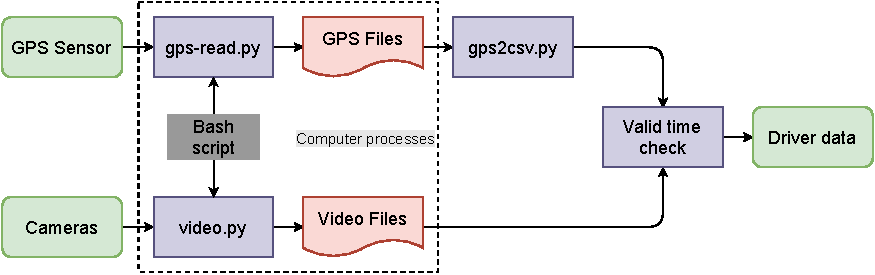
\includegraphics{fig/DAS.pdf}
    \label{fig:das}
    \par SOURCE: The Author (2022).
\end{figure}

The GPS sensor signals were translated into a \verb|.nmea| format file, with the execution of \verb|gps-read.py|. To analyze the collected data, \verb|gps2csv.py| was used by the NDS-BR researchers to translate the \verb|.nmea| into a \verb|.csv| file \cite{Pereira2020}. The GPS registered information including latitude and longitude coordinates, date, time, speed, heading, and altitude. The video files from all cameras were processed by the \verb|video.py| script, having the timestamp and date printed on the screen.

After data was extracted from the laptop, it was necessary to make a valid time check, to exclude times from the final sample where the driver wasn't driving the vehicle. In \autoref{fig:validtime}, it is possible to observe how these invalid times were removed from the sample. For each trip, the period between the start of the car and when the participant started driving was considered invalid. During the trip, if the driver pulled over briefly and then started driving again, this period between the actions was considered as invalid as well. Finally, the gap between parking the car and turning off the DAS was discarded from the sample.  

\begin{figure}[!htbp]
    \centering\footnotesize
    \captionsetup{font=footnotesize}
    \caption{VALID TIME SELECTION}
    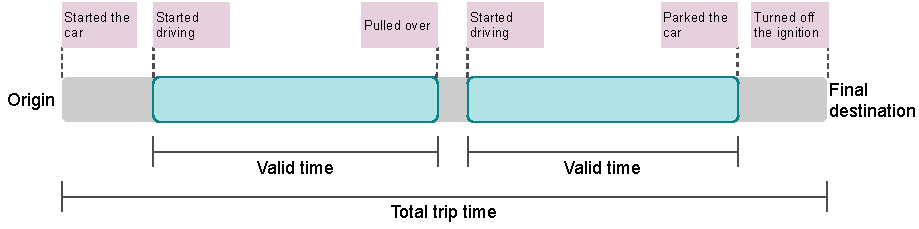
\includegraphics{fig/validtime.pdf}
    \label{fig:validtime}
    \par SOURCE: The Author (2022).
\end{figure}

The first trip of each driver was defined as invalid. This trip was considered to be, to the driver, a time of getting familiar with the monitoring system. Moments with failure on the DAS, where the GPS or video data weren't properly recorded, also were considered invalid time. The process of identifying invalid times was based on manual coding. A group of researchers identified the invalid times using the video data as a reference. 

% 3. Drivers: How many, characteristics, data gathered, duration, how they were selected

% \autoref{tab:drivers} contains information about the participants and their vehicles, including the duration of data collection, age, gender, age of driver's license, vehicle model year, and horsepower.

% \begin{table}[!htbp]
%     \footnotesize
%     \captionsetup{justification=raggedright,
%         singlelinecheck=false,
%         font=footnotesize}
%     \caption{SELECTED PARTICIPANTS INFORMATION}
%     \centering
%     \begin{tabular}{lllllll}
%         \hline
%         \multicolumn{1}{c}{\textbf{ID}} & \multicolumn{1}{c}{\textbf{Duration}} & \multicolumn{1}{c}{\textbf{Age}} & \multicolumn{1}{c}{\textbf{Gender}} & \multicolumn{1}{c}{\textbf{License Age}} & \multicolumn{1}{c}{\textbf{Vehicle year}} & \multicolumn{1}{c}{\textbf{Horsepower}} \\
%         \hline
%         $D_1$    & 13 & 33 & F & 12 & 2012 & 96  \\ % A
%         $D_2$    & 12 & 40 & M & 3  & 2010 & 113 \\ % B
%         $D_3$    & 8  & 22 & M & 3  & 2011 & 103 \\ % C
%         $D_4$    & 16 & 25 & M & 6  & 2003 & 114 \\ % D
%         $D_5$    & 13 & 41 & F & 23 & 2014 & 75  \\ % J
%         $D_6$    & 13 & 28 & M & 9  & 2013 & 163 \\ % K
%         $D_7$    & 17 & 45 & M & 18 & 2011 & 130 \\ % L 
%         $D_8$    & 12 & 32 & F & 10 & 2015 & 79  \\ % M 
%         $D_9$    & 11 & 29 & M & 9  & 2019 & 74  \\ % N 
%         $D_{10}$ & 14 & 62 & M & 37 & 2018 & 69  \\ % O
%         $D_{11}$ & 6  & 28 & F & 10 & 2012 & 75  \\ % P 
%         $D_{12}$ & 5  & 45 & F & 26 & 2001 & 101 \\ % Q
%         $D_{13}$ & 14 & 21 & F & 2  & 2006 & 81  \\ % R 
%         $D_{14}$ & 6  & 34 & M & 16 & 2014 & 124 \\ % W
%         $D_{15}$ & 8  & 49 & F & 24 & 2018 & 84  \\ % X
%         $D_{16}$ & 11 & 27 & M & 3  & 2014 & 109 \\ % Y 
%         \hline
%     \end{tabular}
%     \label{tab:drivers}
%     \par \vspace{2mm} \footnotesize \raggedright
%     SOURCE: The Author (2021)
%     \par \vspace{1mm} \footnotesize \raggedright
%     NOTES: Duration in days; age and license age in years; M-male; F-female
% \end{table}
The NDS-BR data collection started in August 2019. The local of the study is Curitiba and its metropolitan region. Curitiba is the capital city of the State of Paraná, in Brazil. Until December 2021, the project collected data from 32 participants, which composed a sample of naturalistic data used in this thesis. The drivers participated through a survey that was divulged on social networks. The age of the drivers varied between 21 and 63 years old, with 18 females and 14 males. The duration of data collection from each driver varied between 5 and 20 days. Regarding the participants' vehicles, the model year varied between 2001 and 2020, with horsepower varying between 66 and 166 HP. 

Regarding driving experience, the driving license of the participants varied between 2 and 38 years. All participants received a briefing on how to operate the equipment and signed a term of the agreement, allowing the use of their data for academic research purposes. Overall, a total of 1002 trips were performed, resulting in 381.45 hours of driving and 9,443.83 km of traveled distance. Only two drivers had a car with an automatic gearbox. All other drivers had vehicles with a manual gearbox. Four drivers occasionally made trips in carpooling situations, offering rides to passengers with the use of carpooling apps. Three drivers worked as mobility app drivers. Among the participants, 27 lived in Curitiba and 5 lived in the neighboring cities inside the metropolitan region. Their location of residence is mapped in \autoref{fig:address}. 

\begin{figure}[!htbp]
    \centering\footnotesize
    \captionsetup{font=footnotesize}
    \caption{PARTICIPANTS' RESIDENCE LOCATION}
    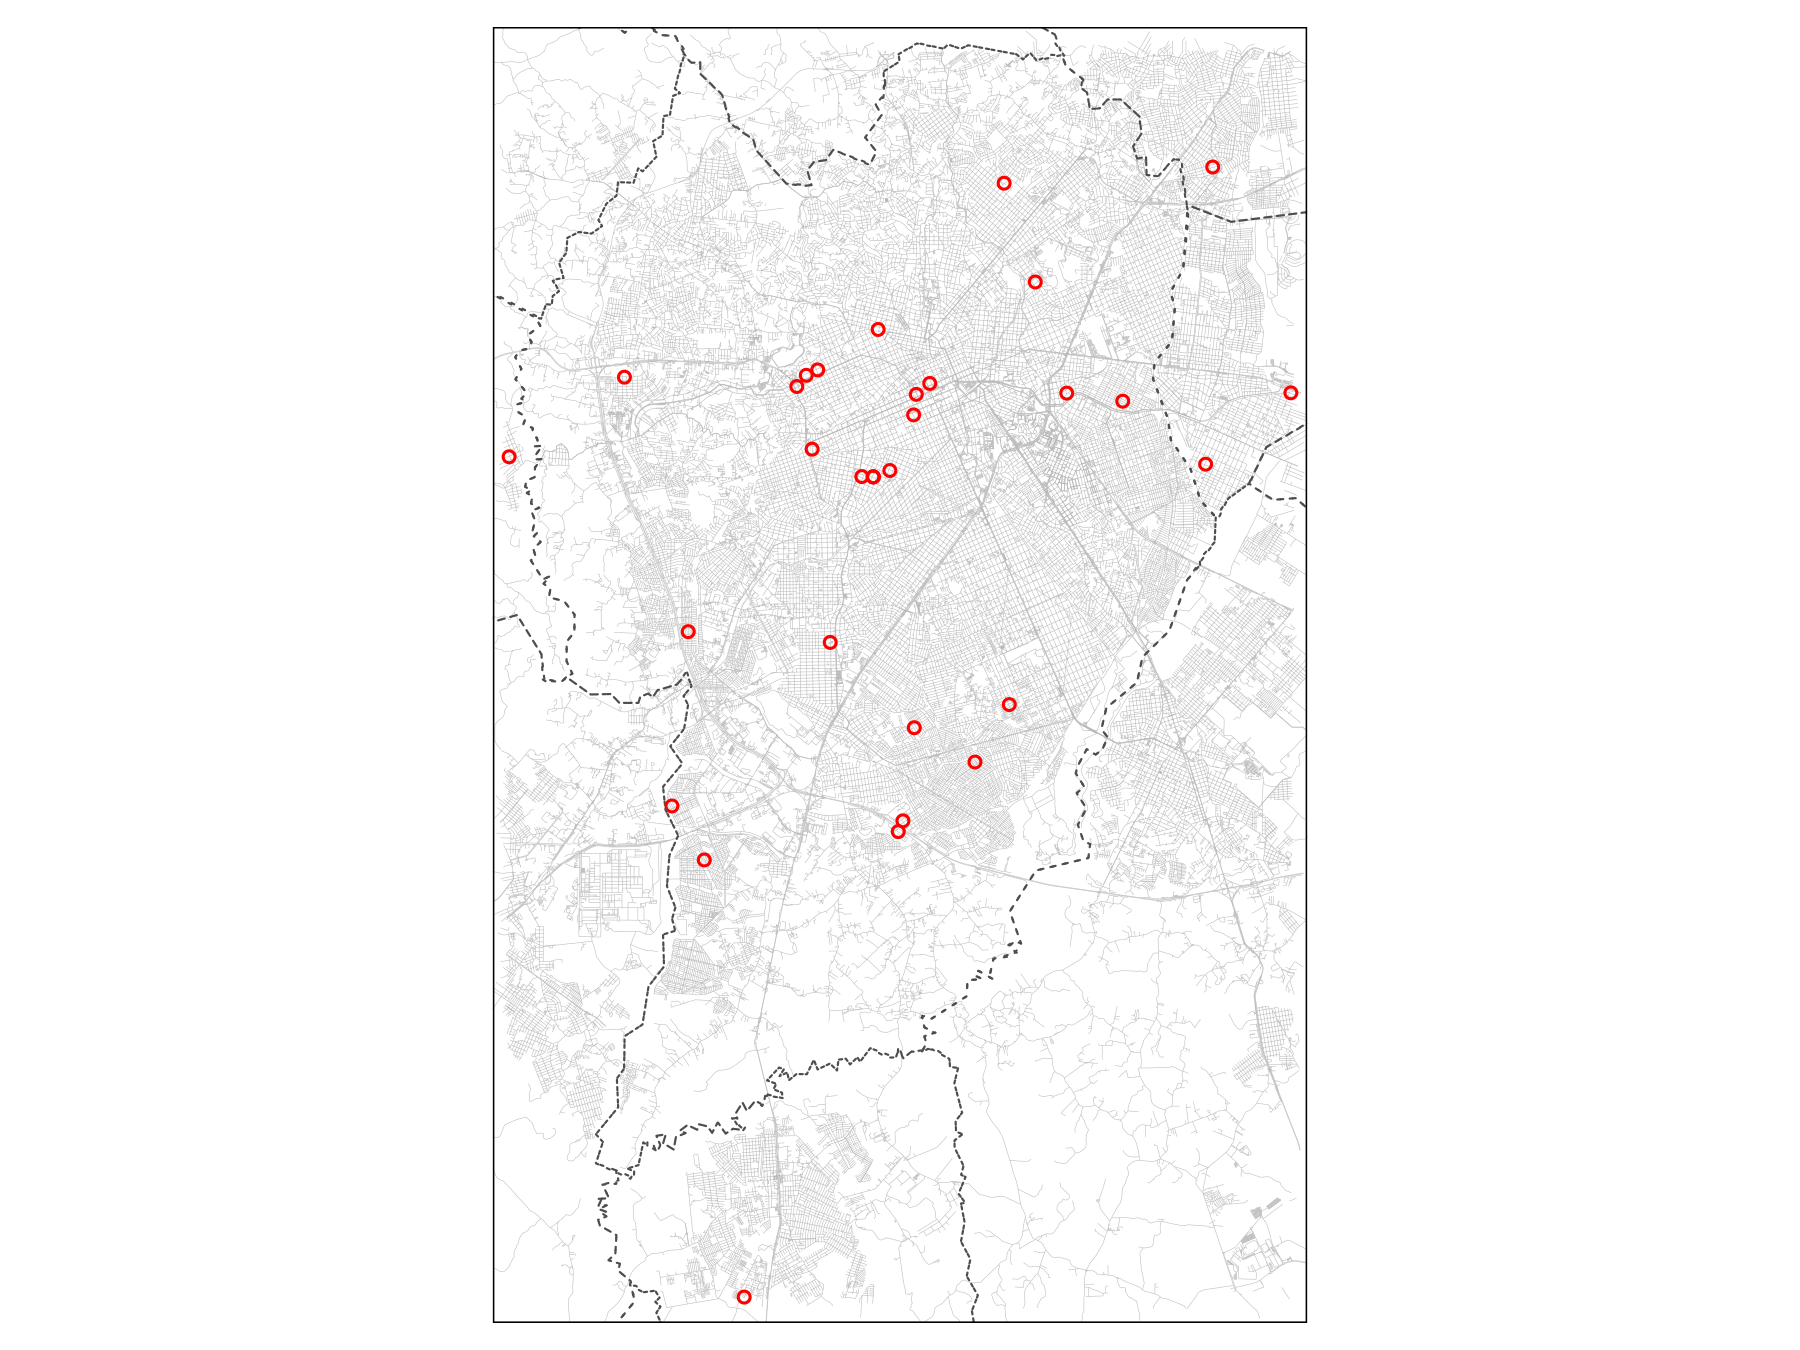
\includegraphics{fig/address_map.png}
    \label{fig:address}
    \par SOURCE: The Author (2022).
\end{figure}

%% Start of NDS, how much time each collected

\section{DATA PROCESSING AND VARIABLE CONSTRUCTION} \label{data}

%% Data processing flowchart

This section includes the methods utilized to construct all the utilized variables, divided into two subsections: the speeding variable (dependent variable) and built environment variables (independent variables). This process is detailed in the following subsections: Subsection \ref{sub:spd} and Subsection \ref{sub:be}.
%  \autoref{fig:methods} includes a brief flowchart on the process of transforming the data sources into a complete dataset included in the traffic analysis zones. 

% \begin{figure}[!htbp]
%     \centering\footnotesize
%     \captionsetup{font=footnotesize}
%     \caption{VARIABLE DATA FLOWCHART}
%     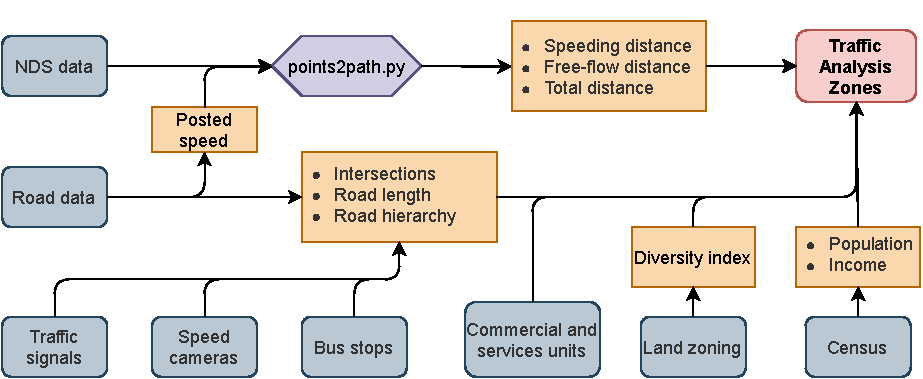
\includegraphics{fig/methods.pdf}
%     \label{fig:methods}
%     \par SOURCE: The Author (2021).
% \end{figure}

\subsection{Speeding} \label{sub:spd}

%% How speeding was measured (NSHTA)

%% How the main dataframe was constructed

% 1. Road axis buffer

% 2. Intersection with nds points

To extract speeding information from the NDS sample, it was necessary to compare the performed speeds from drivers with the respective speed limit. Speed limit data was collected from the road axis in the Shapefile format, obtained from OpenStreetMap \cite{OpenStreetMap}, completing some missing information with speed limits from IPPUC road axis data \cite{IPPUC2021}. A 10-meter buffer was created around each link of the road axes. In sequence, a spatial join between the NDS points and the road buffer was performed to associate the speed limit and the performed speed to the same point in space. All geometrical operations were executed in R, using the \verb|sf| package \cite{pebesma2018}. This process is illustrated in \autoref{fig:buffer}. 

\begin{figure}[!htbp]
    \centering\footnotesize
    \captionsetup{font=footnotesize}
    \caption{ROAD AXIS BUFFER}
    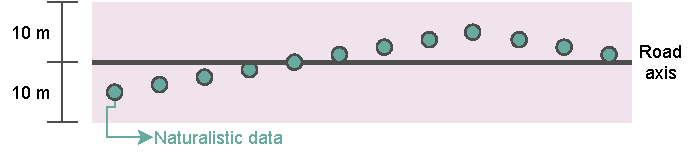
\includegraphics{fig/buffer.pdf}
    \label{fig:buffer}
    \par SOURCE: The Author (2022).
\end{figure}

Points outside the buffers (in the middle of street blocks, for example) were removed from the sample. Also, points without speed limit and performed speed data were removed from the sample. The extraction of free-flow and speeding events followed a method defined by \textcite{Richard2013}, presented in \autoref{fig:ff}. The occurrence of speeding was represented by the proportion of distance traveled in speeds above the speed limit, divided by the distance performed in free-flow speeds. It was necessary to remove sections of the sample where drivers had no opportunity to speed. Therefore, the occurrence of speeding is defined in the following equation: \begin{align}
    SP = \frac{D_{sp}}{D_{f}} \mbox{ ;} 
    \label{eq:sp}
\end{align} where $D_{sp}$ is the distance performed in speeds exceeding 5 km/h above the speed limit (analytical approach) and $D_{f}$ is the distance performed in free-flow speeds. 

In Brazil, a speeding infraction is considered when the driver exceeds the speed limit plus 10\% of the speed limit. Therefore, in a rapid transit road with an 80 km/h speed limit, a driver would be fined if its performed speed reaches above 88 km/h. Considering other urban road hierarchies and limits defined by \textcite{Brasil1997}, speeding in arterial roads (speed limit of 60 km/h) would be considered as speeds above 66 km/h; in collector roads (speed limit of 40 km/h) – speeds above 44 km/h; and local roads – speeds above 33 km/h (speed limit of 30 km/h). Therefore, based on the thresholds of 8 km/h, 6 km/h, 4 km/h, and 3 km/h, it was decided to establish a standard threshold for speeding of 5 km/h above the speed limit. Free-flow speeds included performed speeds higher than the speed limit minus 10 km/h (and lower than the speeding threshold). The free-flow threshold was based on the value established by \textcite{Richard2017} of 5 mph. Direct conversion to km/h would result in 8.05 km/h, therefore it was decided to round the threshold to 10 km/h. $SP$ values can vary between 0 and 1, where 0 represents a section without any speeding, and 1 represents a section traveled only in speeds that exceed the limits. \autoref{fig:spd_occur} contains a representative section of a trip on a road with a 30 km/h speed limit, illustrating the thresholds previously described.   

% 3. Filtering points: speed exposure and speeding - explain criteria (based on richards)

\begin{figure}[!htbp]
    \centering\footnotesize
    \captionsetup{font=footnotesize}
    \caption{SPEEDING OCCURRENCE AND SPEEDING OPPORTUNITY}
    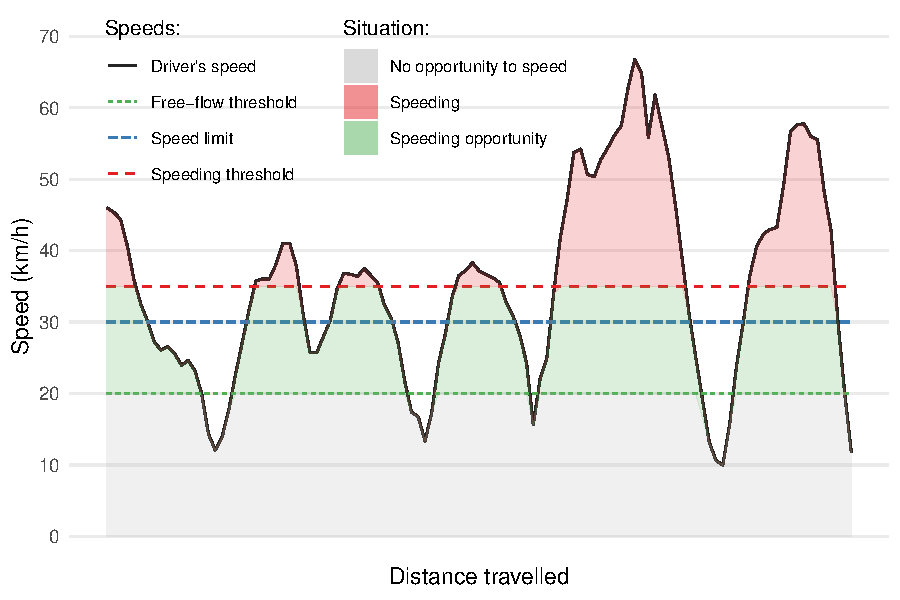
\includegraphics{fig/spd_occur.pdf}
    \label{fig:spd_occur}
    \par SOURCE: The Author (2022).
\end{figure}

% 4. transforming points into lines to export distances: linestring - python script

To calculate distance, a line connecting the GPS coordinates was created. These lines are known as linestrings, a geometry type from the Well-known text (WKT) format. Only points with a 1-second gap from each other (observed from the time variable) were connected with a linestring. Total distances, distances performed in free-flow speeds, and distances in speeding were calculated for each TAZ in Curitiba, to calculate the occurrence of speeding. 

\subsection{Built Environment} \label{sub:be}

%% How the independent variables were calculated

%% How the TAZ shape was constructed

% 1. TAZ shape (general info, source)

All variables (speeding and built environment) were calculated for each traffic analysis zone (TAZ) inside Curitiba. One hundred thirty-five TAZ, established in Curitiba's origin – destination survey made by IPPUC in 2018, was used for this work \cite{IPPUC2018b}. The TAZ is an aggregation of multiple census tracts with similar characteristics inside a defined territory. These tracts were defined in the last census that was executed in Brazil, performed in 2010 \cite{IBGE2010}. The BE variables that were calculated are listed in \autoref{tab:bivar}. Inside the density category, population data were obtained from the last Brazilian Census in 2010 \cite{IBGE2010}. Using the available census tracts, it was possible to calculate the population density (PD) data into the TAZ. 

% 2. Table with all variables: group & variable & abbreviation & unit & expected correlation to speeding

\begin{table}[!htbp]
    \footnotesize
    \captionsetup{justification=raggedright,
        singlelinecheck=false,
        font=footnotesize}
    \caption{BUILT ENVIRONMENT VARIABLES}
    \centering
    \begin{tabular}{lll}
        \hline
        \multicolumn{1}{c}{\textbf{Category}} & \multicolumn{1}{c}{\textbf{Variable}} & \multicolumn{1}{c}{\textbf{Description [unit]}} \\
        \hline
        Density & PD & Population Density [$inhab/km^2$]\\
        Diversity & LDI & Land use diversity index \\
        \multirow[t]{5}*{Design} & DIS & Density of intersections [$no./km$] \\
                              & DSC & Density of speed cameras [$no./km$] \\
                              & TSD & Traffic signal density [$no./km$] \\
                              & PAR & Proportion of arterial roads \\
                              & SND & Street network density [$km/km^2$] \\
        Destination accessibility & DCSU & Density of commercial and services units [$no./km^2$] \\
        Distance to transit & BSD & Bus stop density [$no./km$] \\
        Demographics & AVI & Average income [$BRL$] \\
        \hline
    \end{tabular}
    \label{tab:bivar}
    \par \vspace{2mm} \footnotesize \raggedright
    SOURCE: The Author (2022)
\end{table}

% 3. Independent variables calc (how each one was made) - Insert maps for each variable

Inside the diversity category, the land use diversity index (LDI) was based on  information from Curitiba's zoning plan \cite{Curitiba2019a} as input for its calculation. For each TAZ, the diversity index was calculated based on the following equation \cite{Huang2018}:\begin{align}
    LDI = \frac{-\sum_i^n P_i \times \ln(P_i)}{\ln(n)} \mbox{ ;}
\end{align} where $i$ is the type of land use, $n$ is the total number of land use types in a TAZ, and $P_i$ is the proportional area of land use type $i$. LDI varies between 0 and 1, where 0 represents a single land use zone and 1 represents a perfect distribution of land uses. The GIS data of each zoning type was obtained from \textcite{IPPUC2021}. PD and LDI variables are plotted in \autoref{fig:pd_ldi}.

\begin{figure}[!htbp]
    \centering\footnotesize
    \captionsetup{font=footnotesize}
    \caption{PD AND LDI}
    \begin{subfigure}{0.5\textwidth}
        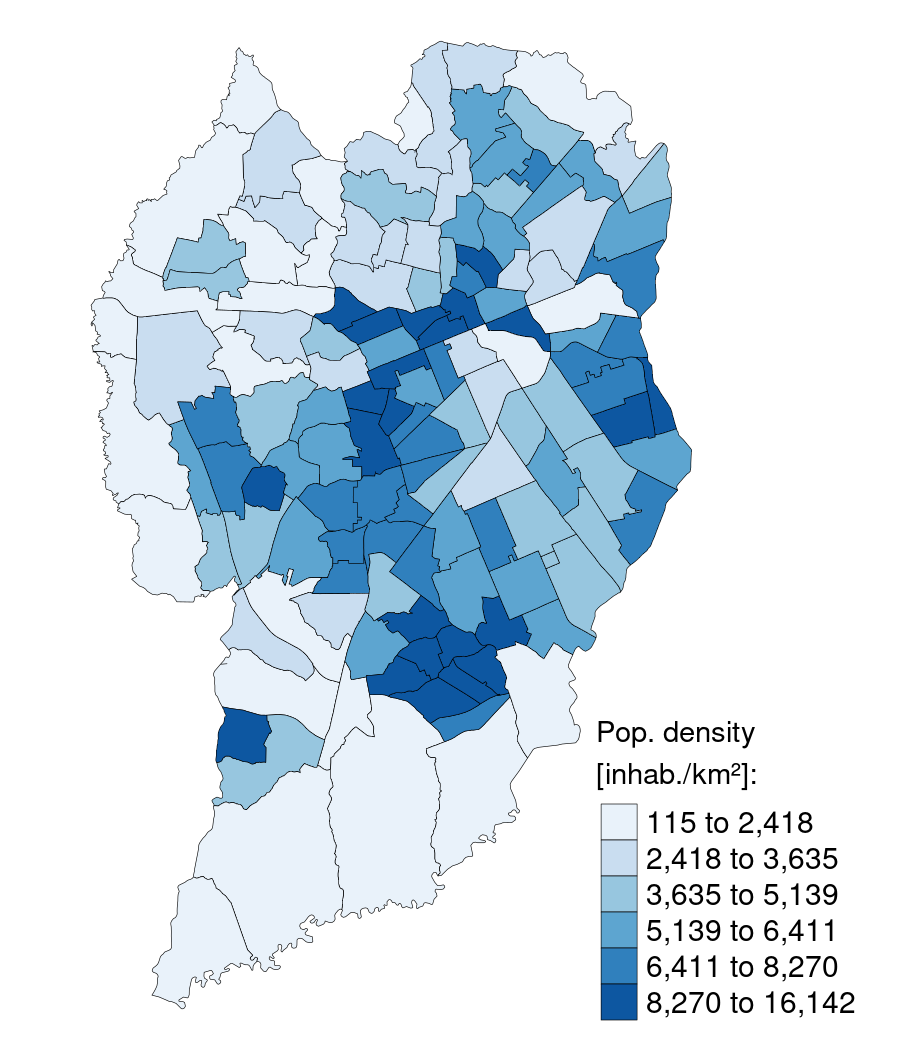
\includegraphics{fig/map_PD.png}
    \end{subfigure}%
    \begin{subfigure}{0.5\textwidth}
        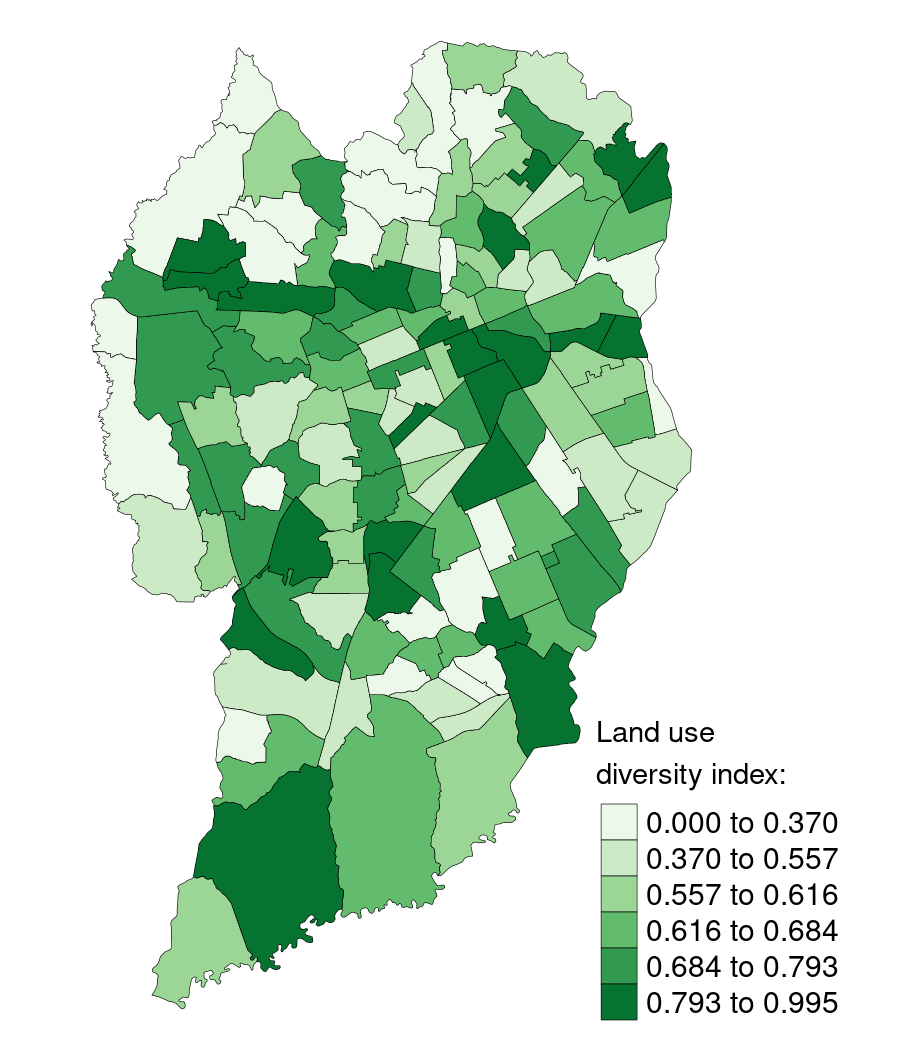
\includegraphics{fig/map_LDI.png}
    \end{subfigure}    
    \label{fig:pd_ldi}
    \par SOURCE: The Author (2022)
\end{figure}

Regarding the design category, the density of intersections (DIS) was calculated based on the number of intersections divided by the length of roads. The intersection points and road lengths were extracted from the \textcite{IPPUC2021} road axis data. Intersection points were extracted using the ``line intersection'' function included in QGIS \cite{QGIS_software}. The density of speed cameras (DSC) and traffic signal density (TSD) computation followed the same method applied to the density of intersections. Speed camera points were obtained from the Municipal Office of Social Defense and Transit of Curitiba \cite{SETRAN2020}, and traffic signal points were obtained from \textcite{IPPUC2021}. DIS and DSC variables are plotted in \autoref{fig:dis_dsc}. 

\begin{figure}[!htbp]
    \centering\footnotesize
    \captionsetup{font=footnotesize}
    \caption{DIS AND DSC}
    \begin{subfigure}{0.5\textwidth}
        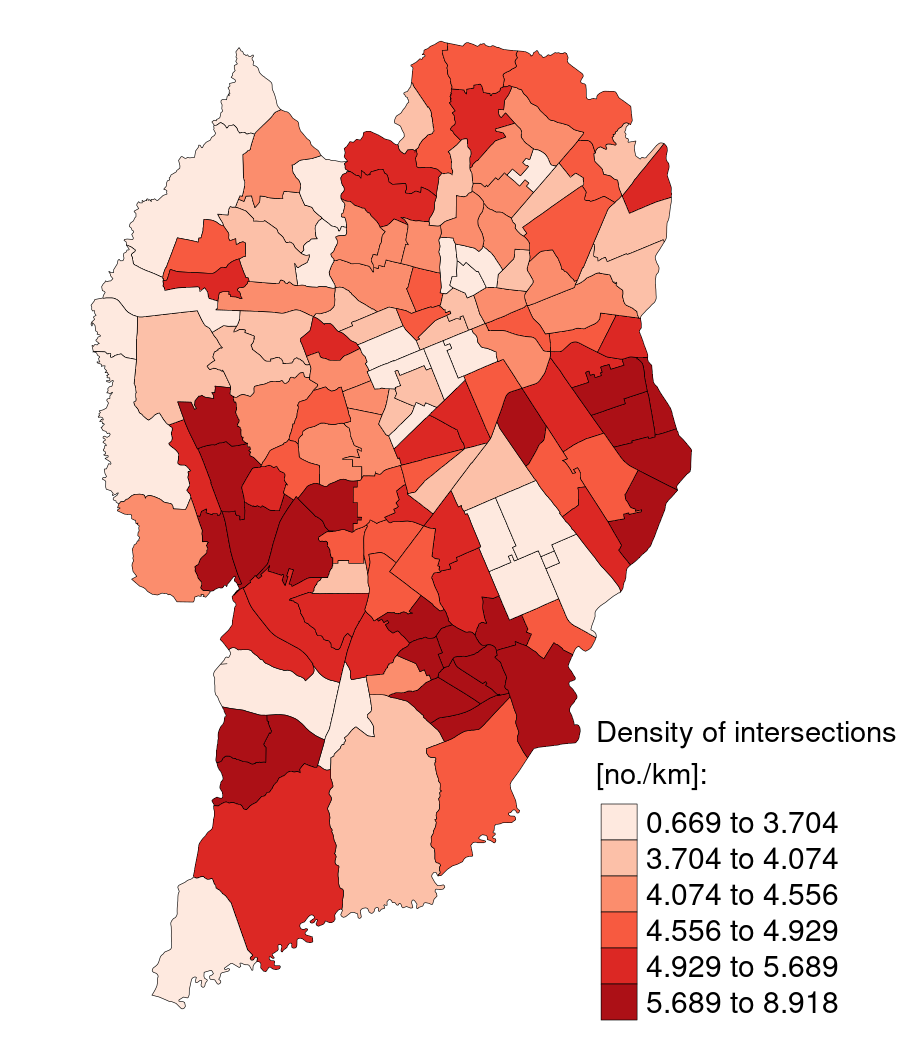
\includegraphics{fig/map_DIS.png}
    \end{subfigure}%
    \begin{subfigure}{0.5\textwidth}
        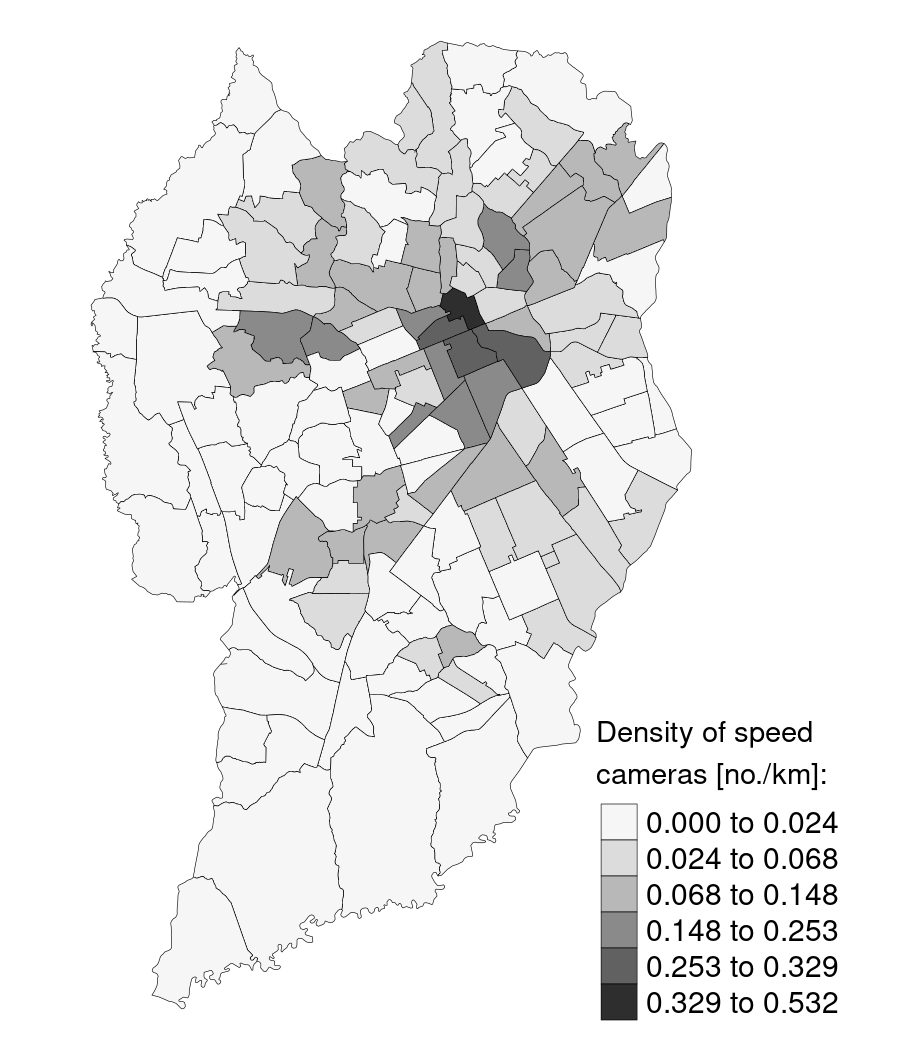
\includegraphics{fig/map_DSC.png}
    \end{subfigure}
    \label{fig:dis_dsc}
    \par SOURCE: The Author (2022), based on \textcite{IPPUC2018b,IPPUC2021,SETRAN2020}
\end{figure}

The proportion of arterial (PAR) was based on the IPPUC road axis data as well. The road hierarchy data followed the categories established by the Brazilian Traffic Code \cite{Brasil1997}: rapid transit, arterial, collector, and local roads. In this variable, rapid transit and arterial roads were combined into one category representing arterial roads. Both rapid transit and arterial roads in Curitiba present a speed limit equal to or above 60 km/h, and both classes of roads have similar physical and operation characteristics, which justifies this union of categories. Hence, the proportion of arterial roads was based on the division between arterial roads length and total road length. TSD and PAR variables are plotted in \autoref{fig:tsd_par}.

\begin{figure}[!htbp]
    \centering\footnotesize
    \captionsetup{font=footnotesize}
    \caption{TSD AND PAR}
    \begin{subfigure}{0.5\textwidth}
        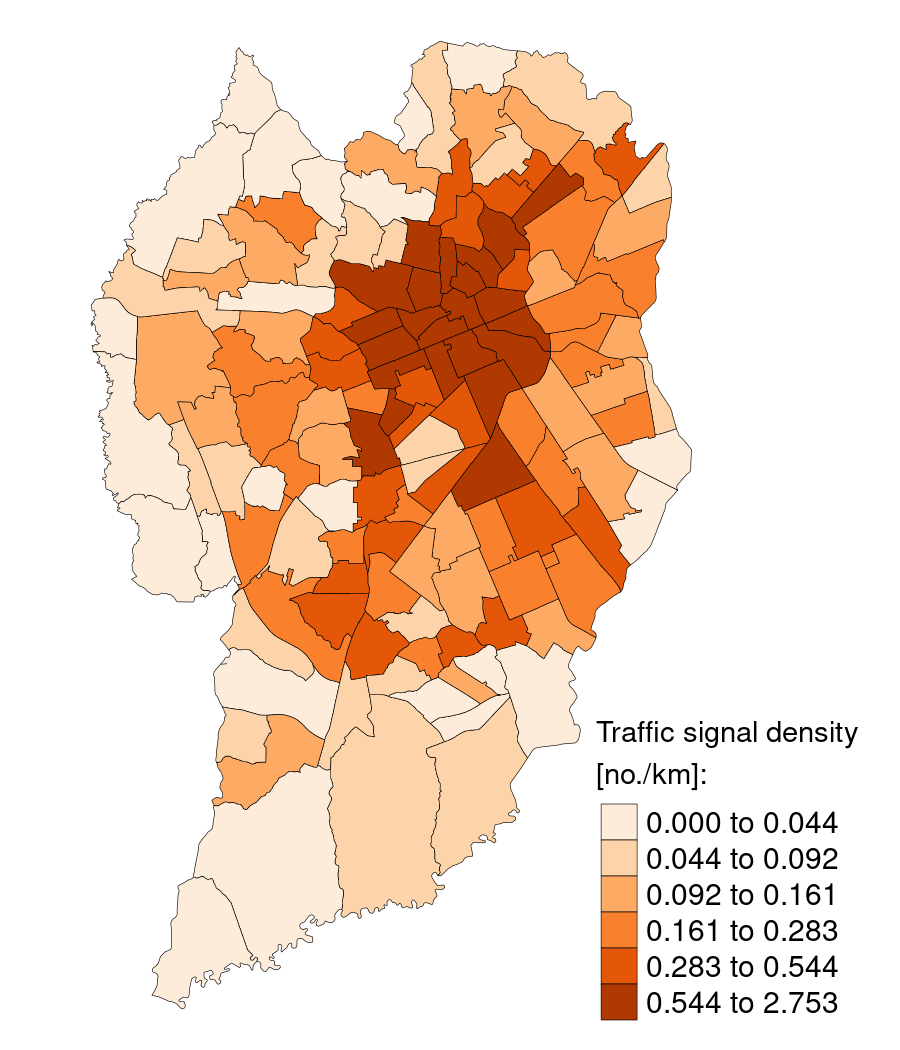
\includegraphics{fig/map_TSD.png}
    \end{subfigure}%
    \begin{subfigure}{0.5\textwidth}
        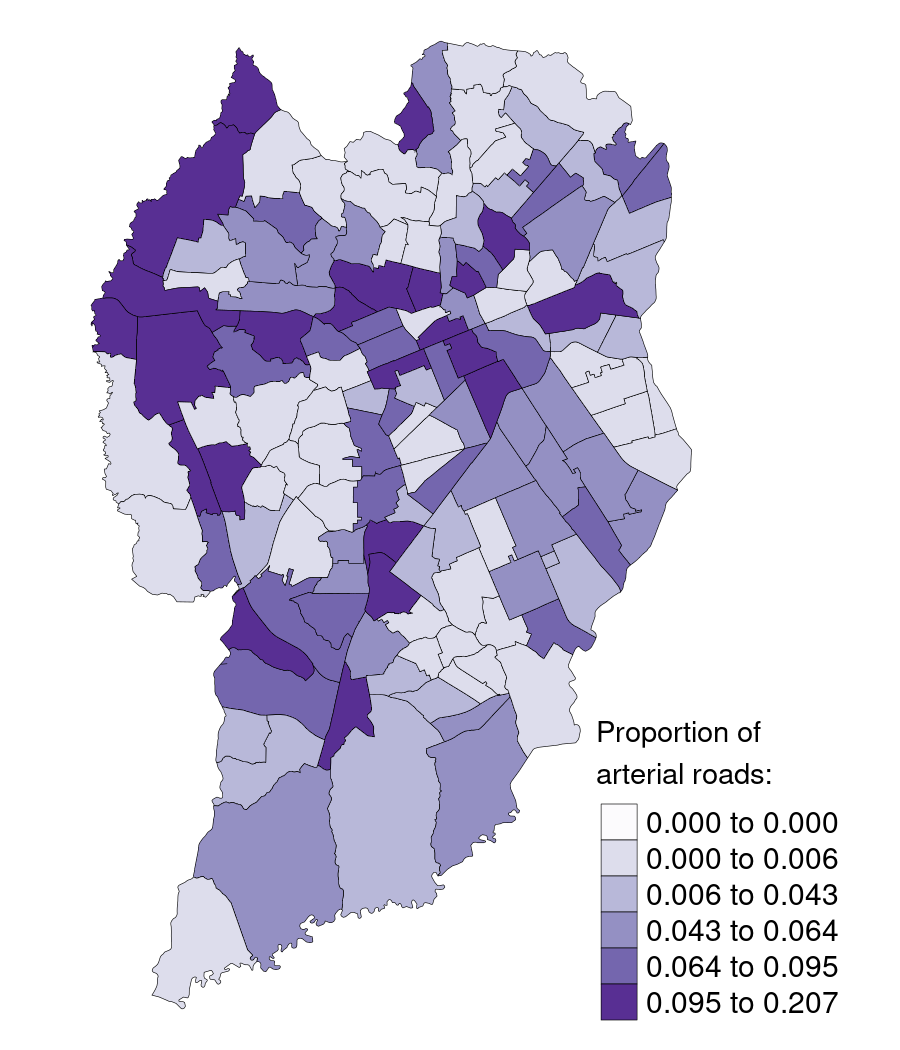
\includegraphics{fig/map_PAR.png}
    \end{subfigure}
    \label{fig:tsd_par}
    \par SOURCE: The Author (2022), based on \textcite{IPPUC2018b,IPPUC2021}
\end{figure}

Street network density (SND) is the total road length divided by the area in square kilometers of the respective TAZ. Regarding the destination accessibility, the location of commercial and services units from 2019 was provided by \textcite{IPPUC2021}, making possible the calculation of the density of commercial and services units (DCSU) per TAZ. SND and DCSU variables are plotted in \autoref{fig:snd_dcsu}.

\begin{figure}[!htbp]
    \centering\footnotesize
    \captionsetup{font=footnotesize}
    \caption{SND AND DCSU}
    \begin{subfigure}{0.5\textwidth}
        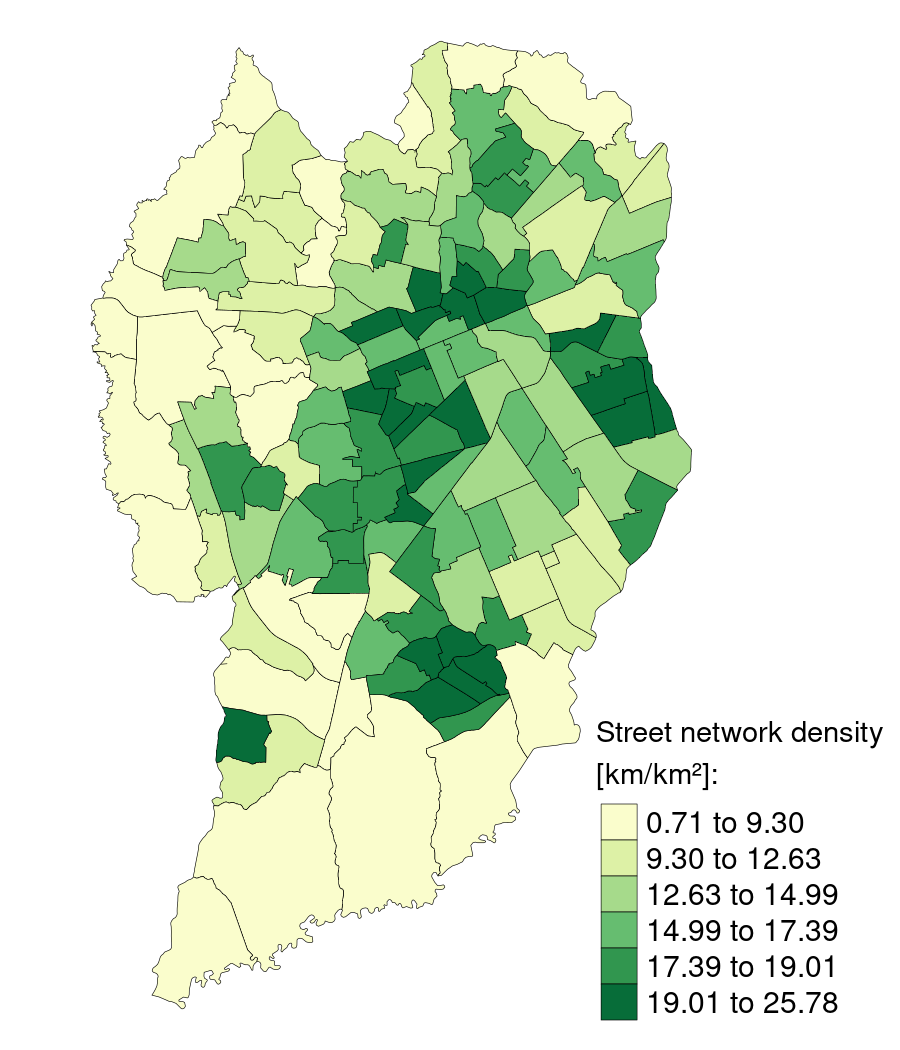
\includegraphics{fig/map_SND.png}
    \end{subfigure}%
    \begin{subfigure}{0.5\textwidth}
        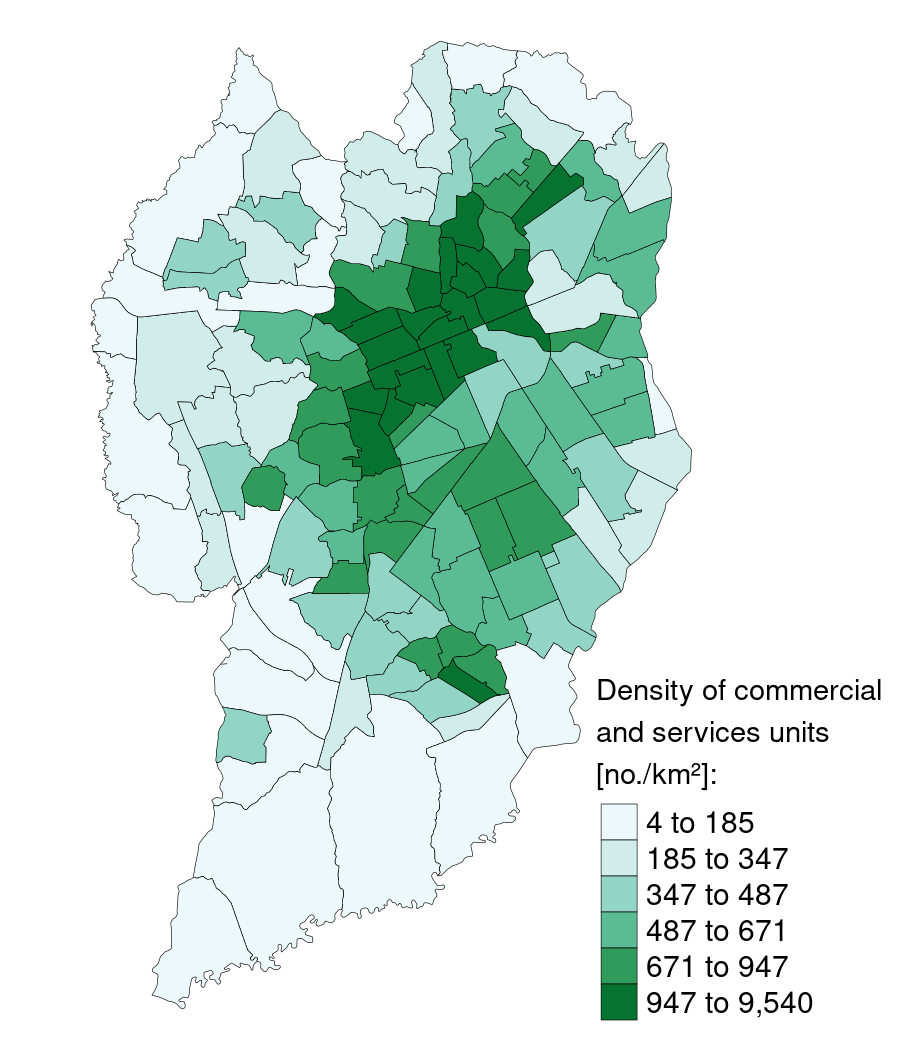
\includegraphics{fig/map_DCSU.png}
    \end{subfigure}
    \label{fig:snd_dcsu}
    \par SOURCE: The Author (2022), based on \textcite{IPPUC2018b,IPPUC2021}
\end{figure}

The distance to transit is represented by the bus stop density (BSD) per road length. The location of bus stops across the city was provided by \textcite{IPPUC2020a}, with data from 2020. Bus stops located in dedicated bus lanes and streets were removed from the sample. The average income (AVI), representing the demographic category, was obtained from the Brazilian Census of 2010 \cite{IBGE2010}. BSD and AVI variables are plotted in \autoref{fig:bsd_avi}. 

\begin{figure}[!htbp]
    \centering\footnotesize
    \captionsetup{font=footnotesize}
    \caption{BSD AND AVI}
    \begin{subfigure}{0.5\textwidth}
        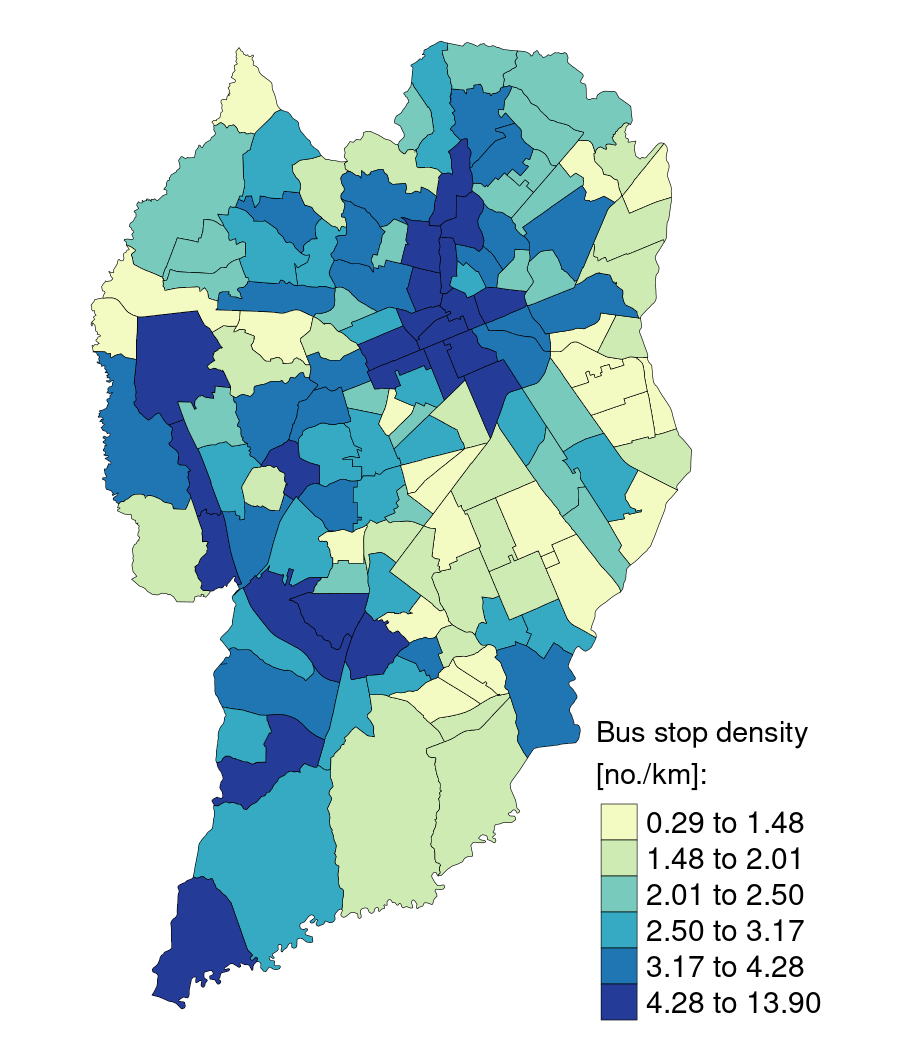
\includegraphics{fig/map_BSD.png}
    \end{subfigure}%
    \begin{subfigure}{0.5\textwidth}
        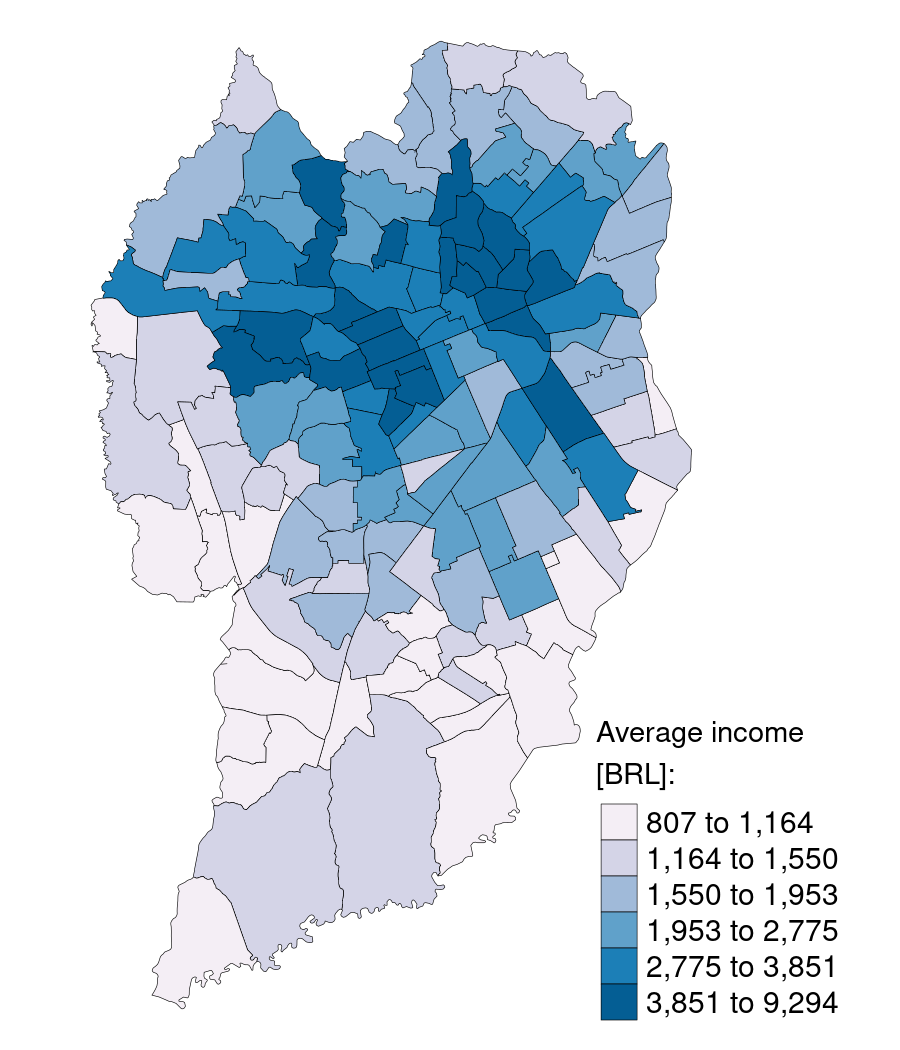
\includegraphics{fig/map_AVI.png}
    \end{subfigure}
    \label{fig:bsd_avi}
    \par SOURCE: The Author (2022), based on \textcite{IPPUC2018b,IPPUC2020a, IBGE2010}
\end{figure}

% \begin{figure}[!htbp]
%     \centering\footnotesize
%     \captionsetup{font=footnotesize}
%     \caption{BSD AND AVI}
%     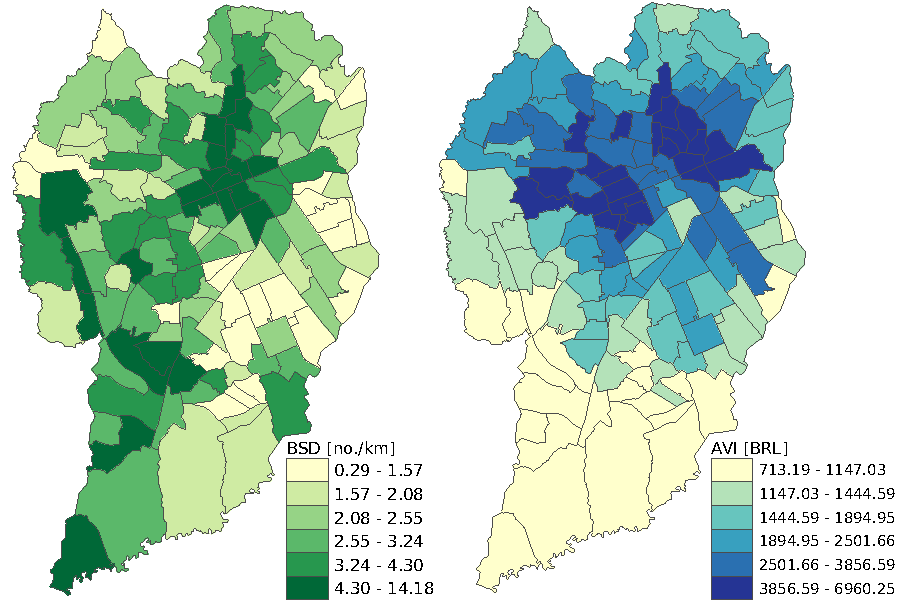
\includegraphics{fig/map_BSD+AVI.pdf}
%     \label{fig:bsd_avi}
%     \par SOURCE: The Author (2021), based on \textcite{IPPUC2018b,IPPUC2020a, IBGE2010}
% \end{figure}

\section{GEOGRAPHICALLY WEIGHTED REGRESSION MODELLING} \label{gwm}

% 1. Filters: free flow_l > 0, prop > 0.1

% 2. 

% 3. 

%% How the model was constructed: Inputs, outputs

%% Describe each possible config (NB, poisson, GLM)

%% Performance measures (AICc, global R-squared, Morans I on residuals)

%% What each function does on code

%% basically a walk through of the code (ref code on appendix)

This section contains the process of modeling a GWR. The steps performed in this section are described in \autoref{fig:gwr-method}. They were implemented using the R programming language as the main tool, with the aid of functions extracted from the \verb|GWmodel| \cite{Gollini2013} and \verb|spdep| \cite{Bivand2013} packages. The TAZ data passed through five main steps to construct and make a diagnostic of the GWR model: data arrangement, bandwidth size selection, kernel type selection, calculation of a global linear model and Moran's $I$ application on the model's residuals. 

\begin{figure}[!htbp]
    \centering\footnotesize
    \captionsetup{font=footnotesize}
    \caption{GWR MODELLING PROCESS}
    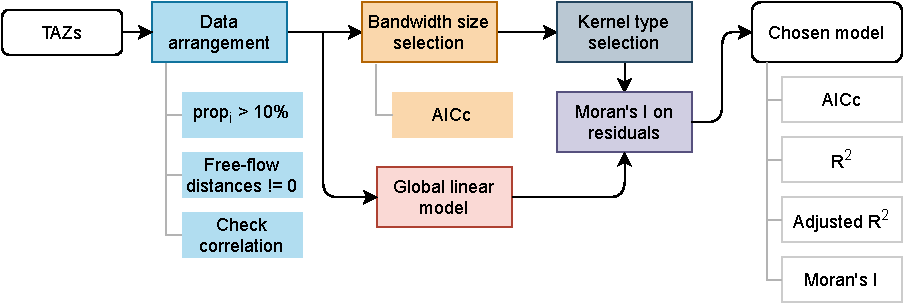
\includegraphics{fig/gwr-method.pdf}
    \label{fig:gwr-method}
    \par SOURCE: The Author (2022).
\end{figure}

The first two steps of the data arrangement process are related to how the naturalistic data of traveled distances are distributed across the TAZ. To check these distances, a new variable was created to represent the proportion of traveled distances per TAZ total road length ($prop_i$). This variable is defined in the following equation: \begin{align}
    prop_i = \frac{D_i}{R_i} \mbox{ ;}
\end{align} where $D_i$ is the distance traveled in the $i$-th TAZ and $R_i$ is the total road length inside the $i$-th TAZ. Hence, all TAZ with a value above 10\% were kept in the sample. This process was made to keep TAZ with a significant amount of travel data.

The second step of data arrangement was the exclusion of TAZ without free-flow episodes. Distances performed in free-flow speed corresponds to the exposure variable of the speeding variable. TAZ with zero free-flow distances could not be used in the process of calculating speeding, therefore they were removed from the sample. Finally, Spearman correlation was performed between all the independent variables. This correlation is based on the following equation \cite{Dodge2010}: \begin{align}
    \rho = 1 - \frac{6 \sum d_i^2}{n \left( n^2 - 1\right)} \mbox{ ;}
\end{align} where $d_i$ is the difference between two ranks of $i$-th observations from different variables and $n$ is the total number of observations. The inclusion of independent variables with correlations above 0.8 can influence negatively the quality of the GWR model \cite{Gollini2013}. Therefore, variables with a Spearman correlation above 0.8 were removed from the sample. 

Considering the variability of TAZ sizes in the sample, the adaptive bandwidth has better performance than a fixed bandwidth \cite{Huang2018}, therefore an adaptive bandwidth was used in this work. To choose the best kernel type, it was necessary to calculate the adaptive bandwidth size (number of neighbors) for each kernel type (gaussian, bisquare, tricube, boxcar, and exponential). The \verb|GWmodel| package in R has a function (\verb|bw.gwr|) for automatic bandwidth selection. This function runs multiple GWR models with multiple bandwidth values and extracts the bandwidth size for the GWR model with the lowest value of corrected Akaike Information Criterion ($AIC_c$) \cite{Gollini2013}.

Minimizing $AIC_c$ to select the bandwidth provides a trade-off between goodness of fit and degrees of freedom. \cite{Fotheringham2002}. For GWR, $AIC_c$ is defined as: \begin{align}
    AIC_c = 2n\log_{e}\left(\hat\sigma\right) + n \log_{e}\left(2\pi\right) + n\left\{\frac{n + \Tr(S)}{n - 2 - \Tr(S)}\right\} \mbox{ ;}
\end{align} where $n$ is the sample size, $\hat\sigma$ is the estimated standard deviation of the error term and $\Tr(S)$ is the trace of the hat matrix, which depends on the bandwidth \cite{Fotheringham2002}. With the discovered optimal bandwidths, the basic form of GWR, presented previously in \autoref{eq:gwr}, was performed five times, one for each type of kernel (\autoref{tab:kernel}). The application of the GWR method utilized the \verb|gwr.basic| function of the \verb|GWmodel| package. In addition, a global linear regression was performed to compare the results with GWR. It was necessary because it is important to verify if the GWR model has an advantage over an ordinary least squares (OLS) approach \cite{Brunsdon2010}. The OLS approach also gives a diagnostic ($p$-value) for each estimated coefficient, which GWR is incapable to do.

Moran's $I$ was applied to the models' residuals to examine the presence of spatial autocorrelation. It is designed to reject the null hypothesis of spatial randomness in favor of an alternative of clustering \cite{anselinLocalSpatialAutocorrelation2020}. A regression model with a good spatial analysis performance shows a lack of spatial autocorrelation on its residuals. The results of Moran's $I$ test varies between -1 and 1, where -1 represents a perfect dispersion pattern and 1 represents a perfect clustering pattern of the data. Results close to 0 and / or without the desired statistical significance ($p$-value) represent a lack of spatial autocorrelation. Moran's $I$ consist of the following equation \cite{Getis2010}: \begin{align}
    I = \frac{n}{W} \times \frac{\sum_i \sum_j w_{ij} (x_i - \overline{x})(x_j - \overline{x})}{\sum_i (x_i - \overline{x})^2} \mbox{ ;}
    \label{eq:global_moran}
\end{align} where $n$ is the sample size, $w_{ij}$ is the matrix of spatial weights, $W$ is the sum of all $w_{ij}$, $x$ is the variable of interest, indexed by $i$ and $j$. and $\overline{x}$ is the mean of $x$. This test was applied using the \verb|moran.test| function included in the \verb|spdep| package \cite{Bivand2013}. The final step was to analyze the performance between models. This analysis was based on four performance indicators: $AIC_c$, $R^2$, adjusted $R^2$, and the value of Moran's $I$ on residuals. Higher values of $R^2$ and adjusted $R^2$ indicate a better performance.

\section{IDENTIFICATION OF CLUSTERS} \label{sec:cluster}

% Explain LISA

% Explain Local Moran

% Explain why / how am I using it. 

The identification of clusters in the GWR results and speeding variable is important to investigate hot spots and cold spots in the data, in addition to spatial outliers. For this objective, the Local Moran statistic was applied. Similar to Moran's $I$, Local Moran is a spatial autocorrelation statistic. Moran's $I$ does not provide an indication of the location of the clusters. However, Local Moran, its local counterpart, does. Local Moran statistic is classified as a local indicator of spatial association (LISA). LISA is characterized for providing a spatial autocorrelation statistic for each location. It also establishes a proportional relationship between the sum of the local statistics and a corresponding global statistic \cite{anselinLocalIndicatorsSpatial2010,anselinLocalSpatialAutocorrelation2020}.

To \textcite{anselinLocalSpatialAutocorrelation2020}, most of the global spatial autocorrelation statistics can be expresses as a double sum over the $i$ and $j$ indices of $g_{ij}$: $\sum_i \sum_j g_{ij}$. The $g_{ij}$ variable can be expressed as the combination of a measure of attribute similarity between a pair of observations ($f(x_i, x_j)$) with an indicator for geographical similarity ($w_{ij}$). Its local form is the sum of the relevant expression over the $j$ index, for each location $i$. Therefore, the generic form for a LISA is: \begin{align}
    \sum_j w_{ij} f\left(x_i, x_j\right) \mbox{.}
\end{align} Applying the same method as Moran's $I$, showed in \autoref{eq:global_moran}, the Local Moran statistic to each observation $i$ is: \begin{align}
    I_i = \frac{\sum_j w_{ij} z_i z_j}{\sum_i z_i^2} \mbox{;}
\end{align} where $z$ is the deviation from the mean of the variable of interest $(x - \overline{x})$. The denominator is fixed in the local configuration, therefore, it can be ignored. Replacing the denominator by $c$ and rearranging the equation, the obtained expression is: \begin{align}
    I_i = c \times z_i \sum_j w_{ij} z_j \mbox{;}
\end{align} representing the product of the value at a location $i$ with the weighted sum of the values at neighboring locations $j$.

To address statistical significance, it is possible to calculate a pseudo $p$-value for each location. In this work, results with $p$-values below 0.05 were defined as statistically significant. It is possible to classify significant locations as High-High; Low-Low spatial clusters, and High-Low; Low-High spatial outliers. High-High locations have high values with neighboring locations that also have high values. The same situation applies to Low-Low spatial clusters, but considering low values. High-Low spatial outliers are locations with high values with neighboring locations that have low values. Low-High spatial outliers follow the same rule, but inverting the values. High and low is relative to the mean of the variable, and does not represent an absolute measure. It is important to observe that identified locations of spatial clusters are not actual clusters, but cores of a cluster. The full cluster is composed of the cores and its direct neighbors \cite{anselinLocalIndicatorsSpatial2010}.

The Local Moran statistic was applied in R, with the aid of the \verb|Rgeoda| package \cite{liRgeodaLibrarySpatial2021}. The \verb|local_moran| function was applied to each coefficient of the GWR model, to SP variable, and to other model's parameter, including local $R^2$. The Local Moran statistic utilized the queen contiguity-based spatial weight. The queen criterion defines neighbors as spatial units sharing a common edge and / or vertices. In this configuration, all neighbors contain the same spatial weight \cite{Bivand2013}. 

%-------------------------------------------------------------------------------

\chapter{RESULTS} \label{cap:results}

% Present 

This chapter focus on the results from the NDS-BR (Sections \ref{sec:ndsr} and \ref{sec:spr}), the results from the GWR (Section \ref{sec:gwrr}).

\section{NATURALISTIC DATA} \label{sec:ndsr}
% 1. Results from NDS (how much each driver participated)

%% How much each driver participated: Quantity of trips, length of trips (mean, median, 1q, 3q, max , min) - try table or boxplot

The process of removing invalid times from the total sample and choosing the traveled data that happened in Curitiba resulted in 5,687.70 kilometers of traveled distance and a total of 821 trips, representing a traveled time of 220.35 hours. Incomplete trips – when only a portion of the trip happened inside Curitiba – were kept in the sample, without the sections that were traveled outside the city borders. \autoref{tab:trips} contains a descriptive summary of trip distance and quantity of trips per driver. Overall, all trips in the sample had a mean distance of 6.92 and a median of 4.54 kilometers traveled. The average quantity of trips per driver was 26, with a median value of 24 trips. The range of trips performed by drivers varies from a minimum of 3 trips to a maximum of 56 trips. 

\begin{table}[!htbp]
    \footnotesize
    \captionsetup{justification=raggedright, singlelinecheck=false,
    font=footnotesize}
    \caption{DESCRIPTIVE STATISTICS OF TRIPS}
    \centering
    \begin{tabular}{lrr}
        \hline
         & \multicolumn{1}{c}{\textbf{Distance of trips [km]}} & \multicolumn{1}{c}{\textbf{Quantity per driver}} \\
        \hline
        Mean   &     6.92 & 26 \\
        SD     &    14.08 & 15 \\
        Min.   &     0.01 &  3 \\
        1Q     &     2.25 & 15 \\
        Median &     4.54 & 24 \\
        3Q     &     8.44 & 38 \\
        Max.   &   164.82 & 56 \\
        \hline
        Total  & 5,687.70 & 821 \\
        \hline
    \end{tabular}
    \label{tab:trips}
    \par \vspace{2mm} \footnotesize \raggedright
    SOURCE: The Author (2022)
\end{table}

In \autoref{fig:taz_drivers} is displayed a map of the quantity of drivers that traveled in each TAZ. Zones closer to the city center show a higher amount of passing drivers, reaching a maximum value of 25. Five zones did not have any travel data from drivers. Overall, none of the TAZ presented the total amount of drivers (32) included in the sample.

\begin{figure}
    \centering\footnotesize
    \captionsetup{font=footnotesize}
    \caption{QUANTITY OF DRIVERS THAT TRAVELED PER TAZ}
    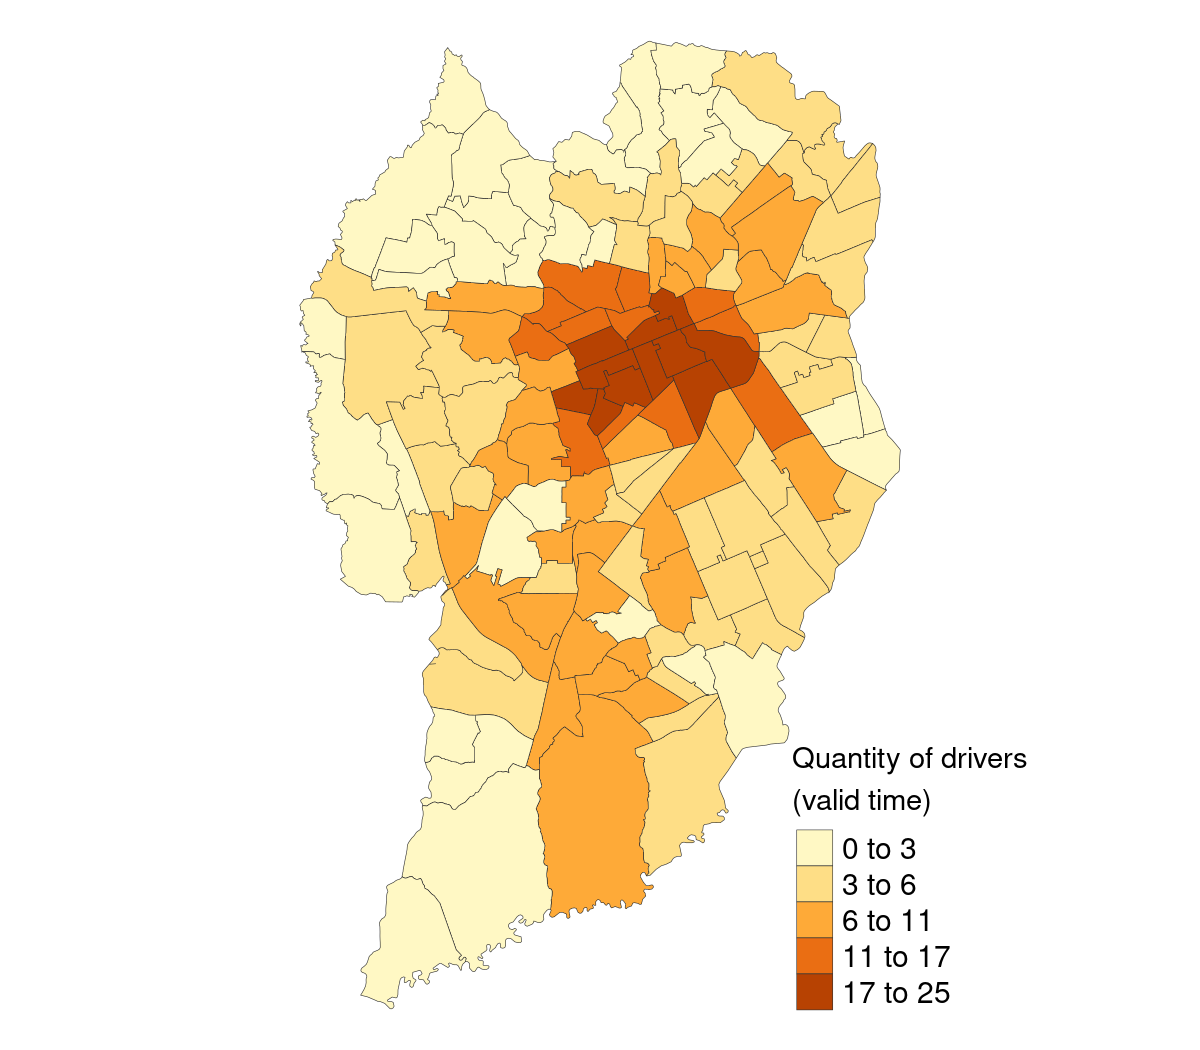
\includegraphics{fig/taz_drivers.png}
    \label{fig:taz_drivers}
    \par SOURCE: The Author (2022)
\end{figure}

In \autoref{fig:dotw_dist}, the distribution of distance traveled per day of the week is presented. Tuesdays had most of the traveled distance, and Saturdays had the least traveled distance. Regarding the trips, \autoref{fig:dotw_trips} contains information on the quantity per day of the week. Wednesdays had the highest amount of trips and Sundays the lowest. Overall, most traveled distances and trips happened in higher amounts during weekdays. \autoref{fig:hotd_dist} and \autoref{fig:hotd_trips} include traveled distance and trip start distribution per hour of the day, respectively.  

\begin{figure}[!htbp]
    \centering\footnotesize
    \captionsetup{font=footnotesize}
    \caption{DISTANCE TRAVELED PER DAY OF THE WEEK}
    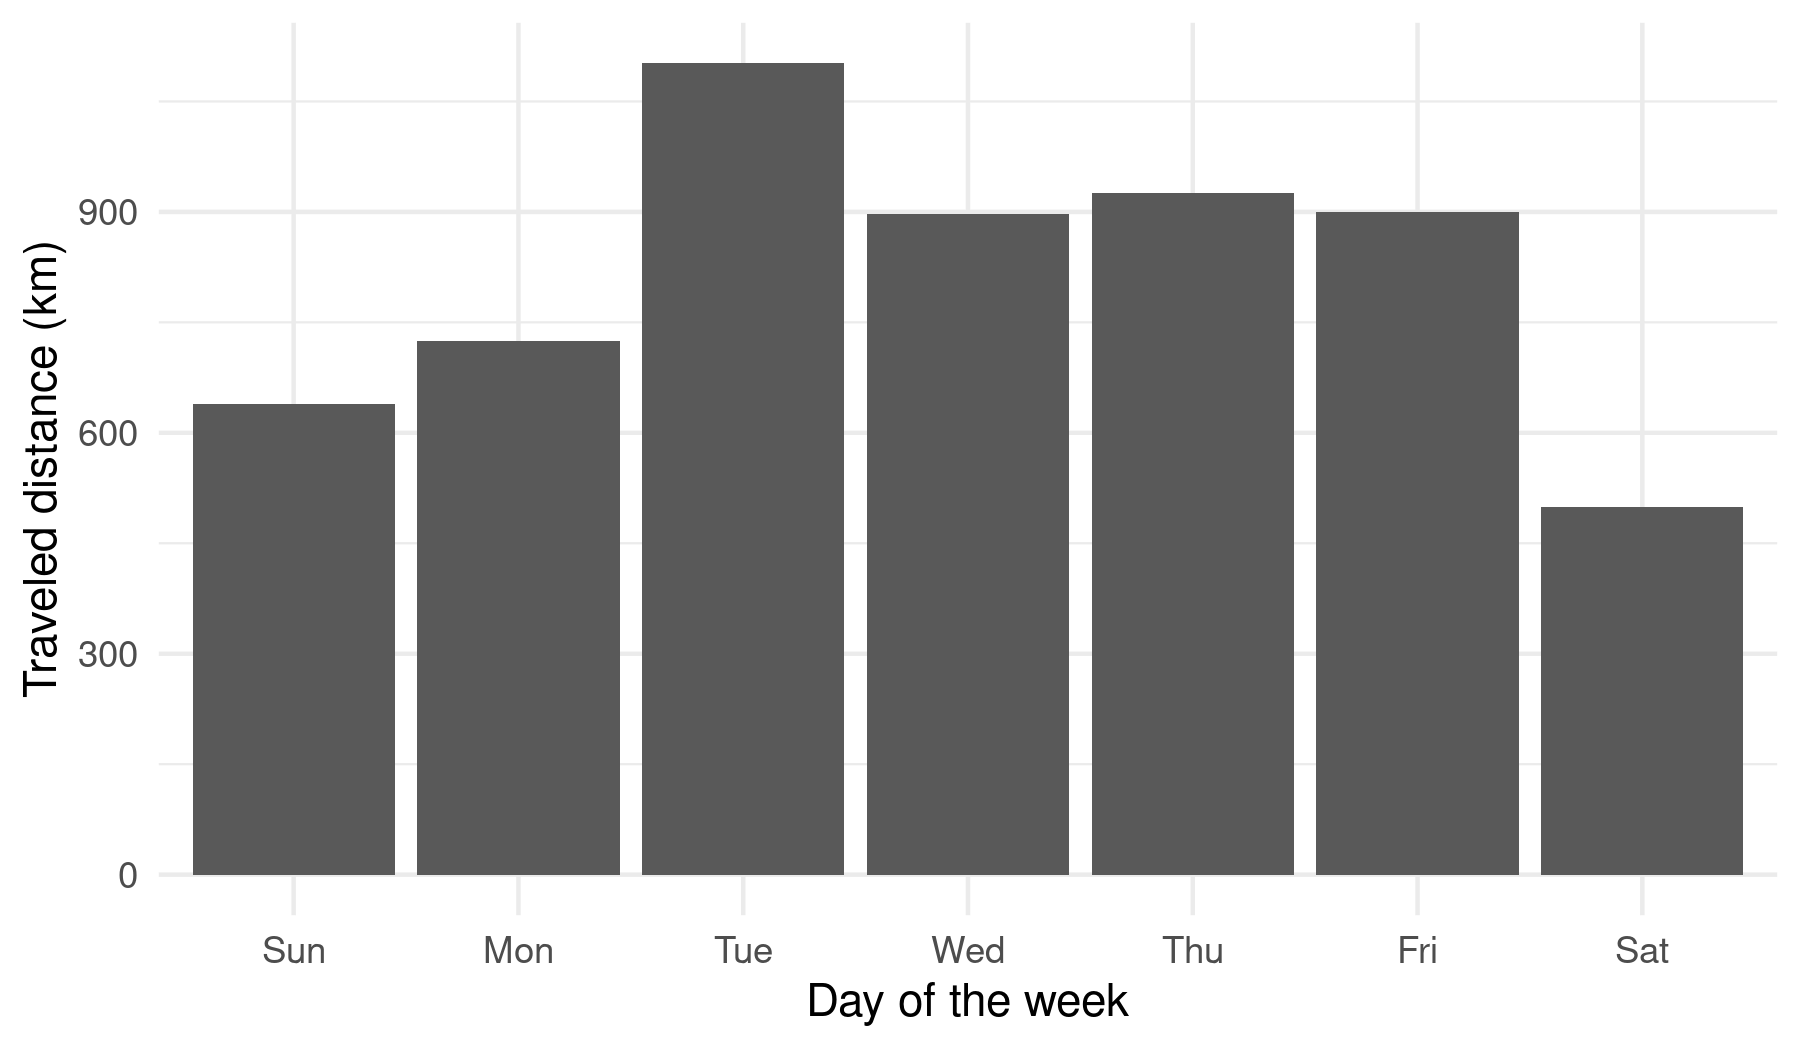
\includegraphics{fig/dotw_dist.png}
    \label{fig:dotw_dist}
    \par SOURCE: The Author (2022)
\end{figure}

%% dotw trips

\begin{figure}[!htbp]
    \centering\footnotesize
    \captionsetup{font=footnotesize}
    \caption{TRIPS PER DAY OF THE WEEK}
    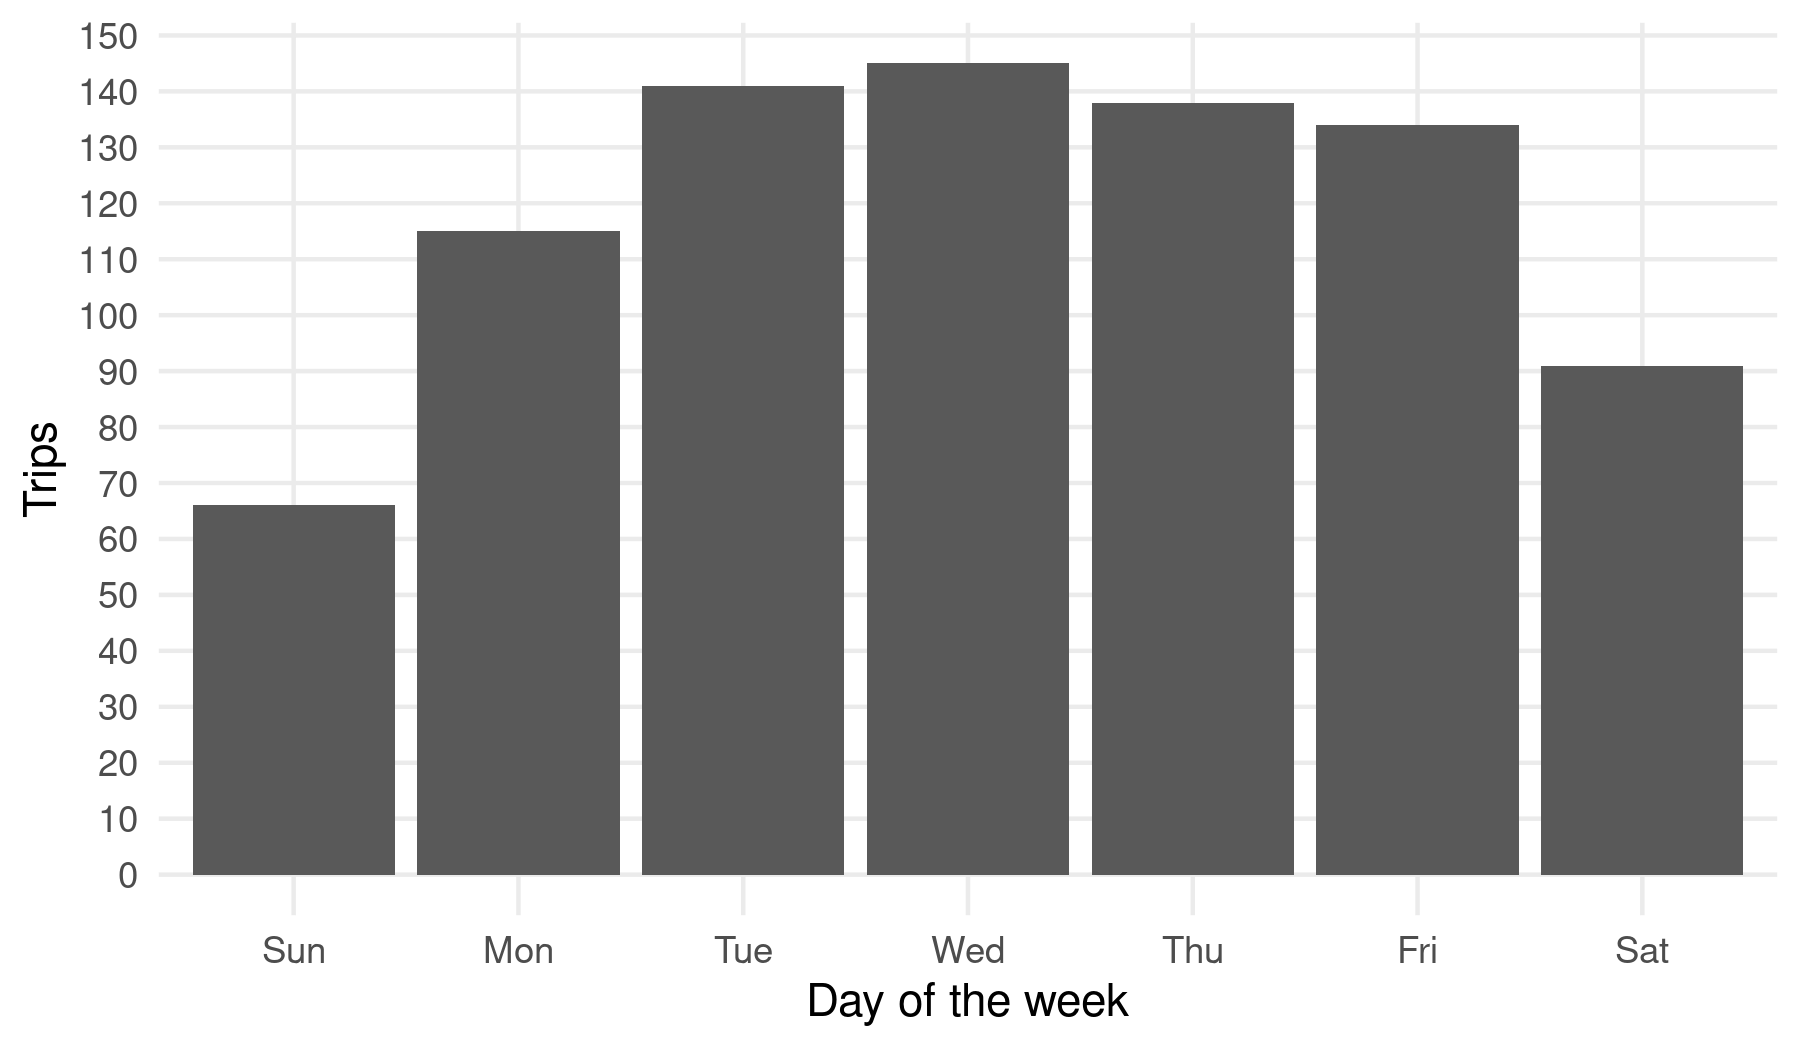
\includegraphics{fig/dotw_trips.png}
    \label{fig:dotw_trips}
    \par SOURCE: The Author (2022)
\end{figure}

%% hotd dist

\begin{figure}[!htbp]
    \centering\footnotesize
    \captionsetup{font=footnotesize}
    \caption{DISTANCE TRAVELED PER HOUR OF THE DAY}
    \includegraphics{fig/hotd_dist.png}
    \label{fig:hotd_dist}
    \par SOURCE: The Author (2022)
\end{figure}

%% hotd trips

\begin{figure}[!htbp]
    \centering\footnotesize
    \captionsetup{font=footnotesize}
    \caption{TRIP START PER HOUR OF THE DAY}
    \includegraphics{fig/hotd_trips.png}
    \label{fig:hotd_trips}
    \par SOURCE: The Author (2022)
\end{figure}

Most of the traveled distance happened between 7:00 – 8:00 and 18:00 – 19:00. Most of the trips started between 7:00 – 8:00, followed by 17:00 – 19:00 and 12:00 – 13:00. \autoref{fig:taz_travel} contains the traveled distance per TAZ in Curitiba. The TAZ with the highest traveled distance had 205.29 kilometers, and the lowest had 0.01 kilometers. Five zones had no traveled distance. Most of the trips happened in central areas of the city.

% how much traveled in each TAZ (MAP)

\begin{figure}[!htbp]
    \centering\footnotesize
    \captionsetup{font=footnotesize}
    \caption{TRAVELED DISTANCE PER TAZ}
    \includegraphics{fig/taz_dist.png}
    \label{fig:taz_travel}
    \par SOURCE: The Author (2022)
\end{figure}

\section{SPEEDING DATA} \label{sec:spr}
% 2. Speeding Results

%% how much speeding for each driver (per trip - mean, median, 1q, 3q, max, min - try table AND boxplot) 

\autoref{tab:speeding} shows the summary of the speeding rate per trip and per driver. The mean speeding rate of trips was 0.39, with a standard deviation of 0.19. The minimum value was 0.00, indicating a trip without speeding, and the maximum value was 1.00, indicating a trip (or a segment of a trip) totally performed in speeding. Regarding the speeding rate per driver, the mean value was 0.44, with a standard deviation of 0.08. The driver with the least speeding presented a value of 0.29, and the driver with the highest level of speeding presented a value of 0.63.

\begin{table}[!htbp]
    \footnotesize
    \captionsetup{justification=raggedright,
        singlelinecheck=false,
        font=footnotesize}
    \caption{DESCRIPTIVE STATISTICS OF SPEEDING RATE PER TRIP AND DRIVER}
    \centering
    \begin{tabular}{lrr}
        \hline
         & \multicolumn{1}{c}{\textbf{Trips}} & \multicolumn{1}{c}{\textbf{Drivers}} \\
        \hline
        Mean   &     0.39 & 0.44 \\
        SD     &     0.19 & 0.08 \\
        Min.   &     0.00 & 0.29 \\
        1Q     &     0.27 & 0.39 \\
        Median &     0.40 & 0.45 \\
        3Q     &     0.52 & 0.51 \\
        Max.   &     1.00 & 0.63 \\
        \hline
    \end{tabular}
    \label{tab:speeding}
    \par \vspace{2mm} \footnotesize \raggedright
    SOURCE: The Author (2022).
\end{table}

%% hour of the day, day of the week (SP)

Speeding values presented a similar value across all days of the week (\autoref{fig:dotw_sp}). Speeding on Tuesdays and Fridays was a bit higher than other days, and on Thursdays and Saturdays, it presented lower values. Regarding the hour of the day (\autoref{fig:hotd_sp}), the highest value of speeding happened between 0:00 – 1:00 and the lowest between 1:00 and 2:00. 

\begin{figure}[!htbp]
    \centering\footnotesize
    \captionsetup{font=footnotesize}
    \caption{SPEEDING PER DAY OF THE WEEK}
    \includegraphics{fig/dotw_sp.png}
    \label{fig:dotw_sp}
    \par SOURCE: The Author (2022)
\end{figure}

\begin{figure}[!htbp]
    \centering\footnotesize
    \captionsetup{font=footnotesize}
    \caption{SPEEDING PER HOUR OF THE DAY}
    \includegraphics{fig/hotd_sp.png}
    \label{fig:hotd_sp}
    \par SOURCE: The Author (2022)
\end{figure}

%% NSHTA diagram of speeding (maybe)

\textcite{Richard2013a} established four types of speeding behavior – situational speeding, incidental speeding, habitual speeding, and casual speeding – based on two variables: percentage of trips with any speeding and average speeding per trip, of each driver. The plotting of these variables and the setting of a zone boundary of 20\% in each variable (arbitrarily defined by \textcite{Richard2013a}) created 4 zones, one for each type of speeding behavior. \autoref{fig:sp_zones} graph manifests the result of this method applied to the speeding sample. In this plot, each dot represents a driver, and its size indicates the number of trips performed by each driver. The y-axis indicates the average speeding per trip of a driver. This speeding was calculated with the $SP$ equation (\ref{eq:sp}) for each trip. The x-axis indicates the percent of trips with any quantity of speeding.

\begin{figure}[!htbp]
    \centering\footnotesize
    \captionsetup{font=footnotesize}
    \caption{TYPES OF SPEEDING BEHAVIOR OF DRIVERS}
    \includegraphics{fig/richards_sp.png}
    \label{fig:sp_zones}
    \par SOURCE: The Author (2022), based on \textcite{Richard2013a}
    \par NOTE: Dot size indicates quantity of trips.
\end{figure}

In \autoref{fig:sp_zones}, it is possible to observe that most of the drivers presented a speeding behavior in at least 80\% of their trips. The average speeding per trip of each driver varied between 20\% and 60\%. All 32 drivers were classified into habitual speeders, in which they regularly speed and have large proportions of speeding in their trips. Situational speeding happens when a high level of speeding per trip happens a few times, indicating that drivers classified in this category usually do not speed. Incidental speeding happens in small proportions of trips and a few trips, representing unintentional speeding events. Casual speeding consists of a higher percentage of trips with any speeding, but with low average speeding behavior per trip.   

\section{GEOGRAPHICALLY WEIGHTED REGRESSION RESULTS} \label{sec:gwrr}

% 3. Results from GWR

%% Show remaining TAZ and remaining sample (distance, time traveled)

The data arrangement process reduced the total sample of 135 TAZ into 117 TAZ. This resulted in a remaining sample of 5,657.25 kilometers of total traveled distance, which includes 3,419.19 kilometers performed in free-flow speeds and 1,508.05 kilometers performed in speeding. In \autoref{fig:taz_filter} a map is presented with the remaining TAZ of the sample. Two removed zones that formed a "hole" in the remaining sample mainly contain industrial zoning. 

\begin{figure}[!htbp]
    \centering\footnotesize
    \captionsetup{font=footnotesize}
    \caption{TAZ CONSIDERED IN THE SAMPLE}
    \includegraphics{fig/map_removal.png}
    \label{fig:taz_filter}
    \par SOURCE: The Author (2022)
\end{figure}

%% Summary of variables: mean, median, max, min, 1q, 3q

In \autoref{tab:var_summary} is included the descriptive statistics of the 11 variables, including speeding, and considering the 117 TAZ. The value of speeding for each TAZ varied between 0.04 and 0.77, with a mean value of 0.46.  DSC, LDI, PAR, and TSD values resulted in zero for some TAZ, indicating a lack of speed cameras, arterial roads, and traffic signals in these zones. The map in \autoref{fig:taz_sp} shows the speeding results for each TAZ, including the Local Moran results for this variable. The Low-Low clusters indicates lower values of SP in 14 zones of the city. Two Low-High outlier were detected between the High-High clusters. Regarding higher values of SP, High-High clusters can be observed at eight different zones. One High-Low cluster was detected. It was also applied a Moran's $I$ statistics on the SP values, which resulted in 0.246 with a $p$-value of 0.001. This is an indication that SP is spatially autocorrelated.

\begin{table}[!htbp]
    \footnotesize
    \captionsetup{justification=raggedright,
        singlelinecheck=false,
        font=footnotesize}
    \caption{DESCRIPTIVE STATISTICS OF VARIABLES}
    \centering
    \begin{tabular}{lrrrrrrr}
        \hline
        \multicolumn{1}{c}{\textbf{Variable [unit]}} & \multicolumn{1}{c}{\textbf{Mean}} & \multicolumn{1}{c}{\textbf{SD}} & \multicolumn{1}{c}{\textbf{Min.}} & \multicolumn{1}{c}{\textbf{1Q}} & \multicolumn{1}{c}{\textbf{Median}} & \multicolumn{1}{c}{\textbf{3Q}} & \multicolumn{1}{c}{\textbf{Max.}} \\ 
        \hline
        % AVI [$BRL$]& 2,628.16 & 1,557.56 & 807.21 & 1,435.00 & 2,087.21 & 3,572.04 & 9,293.81 \\ 
        % BSD [$no./km$] & 3.04 & 2.15 & 0.29 & 1.78 & 2.49 & 3.54 & 13.90 \\ 
        % DCSU [$no./km^2$] & 847.34 & 1,184.30 & 12.30 & 337.76 & 533.36 & 877.57 & 9,539.73 \\ 
        % DIS [$no./km$] & 4.64 & 1.11 & 0.88 & 3.89 & 4.54 & 5.18 & 7.70 \\ 
        % DSC [$no./km$] & 0.06 & 0.09 & 0.00 & 0.00 & 0.03 & 0.08 & 0.53 \\ 
        % LDI & 0.61 & 0.22 & 0.00 & 0.52 & 0.65 & 0.74 & 0.99 \\ 
        % PAR & 0.05 & 0.05 & 0.00 & 0.00 & 0.05 & 0.08 & 0.21 \\ 
        % PD [$inhab./km^2$] & 5,672.35 & 3,113.04 & 114.68 & 3,286.27 & 5,489.84 & 7,244.98 & 16,142.06 \\ 
        % SND [$km/km^2$] & 15.08 & 4.41 & 3.68 & 12.54 & 15.63 & 18.14 & 25.78 \\ 
        % SP & 0.31 & 0.14 & 0.01 & 0.20 & 0.30 & 0.40 & 0.65 \\ 
        % TSD [$no./km$] & 0.37 & 0.48 & 0.00 & 0.09 & 0.20 & 0.40 & 2.75 \\

        AVI [$BRL$] & 2635.66 & 1562.12 & 807.21 & 1407.53 & 2102.42 & 3603.45 & 9293.81 \\ 
        BSD [$no./km$] & 3.05 & 2.15 & 0.29 & 1.79 & 2.50 & 3.55 & 13.90 \\ 
        DCSU [$no./km^2$] & 852.48 & 1188.07 & 12.30 & 340.66 & 536.74 & 881.25 & 9539.73 \\ 
        DIS [$no./km$] & 4.64 & 1.11 & 0.88 & 3.89 & 4.53 & 5.19 & 7.70 \\ 
        DSC [$no./km$] & 0.06 & 0.09 & 0.00 & 0.00 & 0.03 & 0.08 & 0.53 \\ 
        LDI & 0.61 & 0.22 & 0.00 & 0.52 & 0.65 & 0.74 & 0.99 \\ 
        PAR & 0.05 & 0.05 & 0.00 & 0.00 & 0.05 & 0.08 & 0.21 \\ 
        PD [$inhab./km^2$] & 5692.36 & 3118.80 & 114.68 & 3285.42 & 5591.78 & 7248.87 & 16142.06 \\ 
        SND [$km/km^2$] & 15.10 & 4.43 & 3.68 & 12.60 & 15.72 & 18.15 & 25.78 \\ 
        SP & 0.46 & 0.14 & 0.04 & 0.35 & 0.47 & 0.54 & 0.77 \\ 
        TSD [$no./km$] & 0.38 & 0.48 & 0.00 & 0.09 & 0.20 & 0.41 & 2.75 \\ 
        \hline
    \end{tabular}
    \label{tab:var_summary}
    \par \vspace{2mm} \footnotesize \raggedright
    SOURCE: The Author (2022).
\end{table}

%% How much speeding in each TAZ (map)

% \begin{figure}[!htbp]
%     \centering\footnotesize
%     \captionsetup{font=footnotesize}
%     \caption{SPEEDING PER TAZ}
%     \includegraphics{fig/map_SP.png}
%     \label{fig:taz_sp}
%     \par SOURCE: The Author (2021)
%     \par NOTE: Grey areas have no data.
% \end{figure}

\begin{figure}[!htbp]
    \centering\footnotesize
    \captionsetup{font=footnotesize}
    \caption{SPEEDING PER TAZ}
    \begin{subfigure}{0.5\textwidth}
        \includegraphics{fig/taz_SP.png}
    \end{subfigure}%
    \begin{subfigure}{0.5\textwidth}
        \includegraphics{fig/lisa_SP.png}
    \end{subfigure}    
    \label{fig:taz_sp}
    \par SOURCE: The Author (2022)
    \par NOTE: Grey zones have no data.
\end{figure}

%% Show correlogram (remaining variables)

The final step of the data arrangement process was the check of correlation between all independent variables, using the Spearman method. The results of this process are displayed in the correlogram in \autoref{fig:corr_spear}. None of the variables presented a correlation equal to or above 0.8, therefore, all of them were kept in the regression model.  

\begin{figure}[!htbp]
    \centering\footnotesize
    \captionsetup{font=footnotesize}
    \caption{SPEARMAN CORRELOGRAM OF INDEPENDENT VARIABLES}
    \includegraphics{fig/spear.png}
    \label{fig:corr_spear}
    \par SOURCE: The Author (2022)
\end{figure}

%% Show models results (quality variables) - AICc, morans I, R-squared

In \autoref{tab:mod_diag}, the model diagnostics of five GWR and one global linear model is shown, based on 4 performance indicators: $AIC_c$, $R^2$, Adjusted $R^2$, and Moran's $I$ on residuals. The $p$-value indicates the statistical significance of Moran's $I$ results. The global linear regression presented the best $AIC_c$, with a value of -142.372. Regarding $R^2$ and adjusted $R^2$, the GWR model with bisquare kernel showed the best diagnostic, presenting values of 0.342 and 0.195, respectively. The bisquare kernel presented the lowest value of Moran's $I$ on residuals (0.106). All GWR models presented a better performance in comparison to the global linear model when considering the spatial autocorrelation of the residuals, but the global model performed better when considering $AICc$ values. Given that speeding behavior is spatially autocorrelated (\autoref{fig:taz_sp}), it was decided to discard the global linear model in favor of a GWR model. Therefore, the GWR model with the bisquare kernel was selected, having the best $R^2$, adjusted $R^2$ and Moran's $I$ value between the GWR models.

\begin{table}[!htbp]
    \footnotesize
    \captionsetup{justification=raggedright,
        singlelinecheck=false,
        font=footnotesize}
    \caption{MODEL DIAGNOSTICS}
    \centering
    \begin{tabular}{llrrrrrr}
        \hline
        \multicolumn{1}{c}{\textbf{Model}} & \multicolumn{1}{c}{\textbf{Kernel}} & \multicolumn{1}{c}{\textbf{$AIC_c$}} & \multicolumn{1}{c}{\textbf{$R^2$}} &
        \multicolumn{1}{c}{\textbf{Adj. $R^2$}} & \multicolumn{1}{c}{\textbf{Moran's $I$}} & \multicolumn{1}{c}{\textbf{$p$-value}} & \multicolumn{1}{c}{\textbf{Bandwidth}} \\
        \hline
        GWR & Gaussian    & -141.905 & 0.282 & 0.186 & 0.130 & 0.013 & 115 \\
            & Bisquare    & -138.502 & 0.342 & 0.195 & 0.106 & 0.031 & 115 \\
            & Tricube     & -136.661 & 0.324 & 0.192 & 0.112 & 0.028 & 115 \\
            & Boxcar      & -141.828 & 0.273 & 0.190 & 0.122 & 0.016 & 105 \\
            & Exponential & -141.122 & 0.324 & 0.190 & 0.121 & 0.018 & 115 \\
        Global linear & - & -142.372 & 0.262 & 0.192 & 0.137 & 0.008 & -   \\
        \hline
    \end{tabular}
    \label{tab:mod_diag}
    \par \vspace{2mm} \footnotesize \raggedright
    SOURCE: The Author (2022).
\end{table}

In \autoref{tab:lm_results}, the coefficient estimates of the linear regression model are shown, in addition to the standard error, $t$-values, and $p$-values. The only statistically significant coefficient at the 95\% level was the proportion of arterial roads (PAR), which expressed an inverted correlation to speeding. It is necessary to observe the $p$-values of the linear model to identify statistical significance of the GWR parameter estimates, considering that GWR does not have a diagnostic value to analyze coefficient significance (e.g., $p$-value). 

%% Show lm results

\begin{table}[!htbp]
    \footnotesize
    \captionsetup{justification=raggedright,
        singlelinecheck=false,
        font=footnotesize}
    \caption{SUMMARY OF LINEAR MODEL ESTIMATES}
    \centering
    \begin{tabular}{lrrrr}
        \hline
        \multicolumn{1}{c}{\textbf{Coefficient}} & \multicolumn{1}{c}{\textbf{Estimate}} & \multicolumn{1}{c}{\textbf{Std. Error}} & \multicolumn{1}{c}{\textbf{$t$-value}} & \multicolumn{1}{c}{\textbf{$p$-value}}  \\
        \hline
        Intercept  &  5.362e-01 & 8.322e-02 &  6.444 &  3.52e-09 \\
        TSD        & -5.747e-02 & 5.425e-02 & -1.059 &  0.2919   \\
        PAR        & -5.743e-01 & 2.864e-01 & -2.005 &  0.0475*  \\ 
        DCSU       & -9.240e-06 & 1.842e-05 & -0.502 &  0.6169   \\ 
        AVI        & -2.949e-06 & 8.748e-06 & -0.337 &  0.7367   \\ 
        BSD        & -1.781e-03 & 7.530e-03 & -0.236 &  0.8135   \\ 
        LDI        &  6.655e-02 & 5.754e-02 &  1.156 &  0.2501   \\ 
        DSC        & -2.636e-01 & 1.919e-01 & -1.374 &  0.1724   \\ 
        SND        & -3.196e-03 & 4.646e-03 & -0.688 &  0.4930   \\ 
        PD         &  1.106e-06 & 6.756e-06 &  0.164 &  0.8703   \\ 
        DIS        &  3.565e-03 & 1.470e-02 &  0.243 &  0.8088   \\ 
        \hline
    \end{tabular}
    \label{tab:lm_results}
    \par \vspace{2mm} \footnotesize \raggedright
    SOURCE: The Author (2022).
    \par 
    NOTE: * Significance at 95\%
\end{table}

%% Show GWR results

In \autoref{tab:gwr_results}, the descriptive statistics of the chosen GWR model coefficient estimates are showed. The map in \autoref{fig:gwr_par} shows PAR coefficients in each TAZ (the only variable that presented statistical significance), in addition to the Local Moran clusters results. The other nine coefficients are presented in APPENDIX 1. \autoref{fig:r2_map} shows the variation of local geographically weighted $R^2$. Local Moran results shows a cluster with higher values in the northeastern part of the city and another cluster with low values in west and south parts of the city. Local $R^2$ values varied between 0.267 and 0.444. 

\begin{table}[!htbp]
    \footnotesize
    \captionsetup{justification=raggedright,
        singlelinecheck=false,
        font=footnotesize}
    \caption{DESCRIPTIVE STATISTICS OF GWR COEFFICIENT ESTIMATES}
    \centering
    \begin{tabular}{lrrrrr}
        \hline
        \multicolumn{1}{c}{\textbf{Coefficient}} & \multicolumn{1}{c}{\textbf{Min.}} & \multicolumn{1}{c}{\textbf{1Q}} & \multicolumn{1}{c}{\textbf{Median}} & \multicolumn{1}{c}{\textbf{3Q}} & \multicolumn{1}{c}{\textbf{Max.}} \\
        \hline
        % Intercept & 2.665e-01 & 3.611e-01 & 3.852e-01 & 4.135e-01 & 5.243e-01 \\ 
        % PAR & -1.756e+00 & -1.524e+00 & -1.258e+00 & -1.044e+00 & -7.092e-01 \\ 
        % TSD & -1.532e-01 & -8.966e-02 & -8.090e-02 & -6.832e-02 & -3.597e-02 \\
        % DCSU & -2.206e-05 & -1.386e-05 & -1.136e-05 & -5.634e-06 & -7.798e-07 \\
        % LDI & 3.382e-02 & 7.092e-02 & 1.014e-01 & 1.595e-01 & 2.232e-01 \\ 
        % BSD & -5.262e-03 & 4.542e-03 & 9.462e-03 & 1.098e-02 & 1.944e-02 \\
        % DSC & -2.925e-01 & -1.801e-01 & -1.312e-01 & -1.110e-01 & -1.491e-02 \\
        % AVI & -1.039e-05 & -4.306e-06 & -1.686e-06 & 3.367e-06 & 9.646e-06 \\
        % PD & -2.946e-06 & 2.869e-07 & 1.847e-06 & 3.676e-06 & 7.650e-06 \\
        % SND & -8.173e-03 & -5.163e-03 & -3.893e-03 & -1.406e-03 & 2.626e-03 \\
        % DIS & -1.961e-02 & -1.046e-02 & -8.472e-03 & 1.565e-03 & 2.257e-02 \\
        Intercept & 4.5052e-01 & 4.8525e-01 & 5.1751e-01 & 5.4015e-01 & 0.5908 \\
        TSD       & -1.0215e-01 & -6.8228e-02 & -5.8685e-02 & -4.7568e-02 & -0.0180 \\
        PAR       & -1.1447e+00 & -9.6812e-01 & -7.9620e-01 & -6.4543e-01 & -0.5257 \\
        DCSU      & -2.1754e-05 & -1.5861e-05 & -1.3686e-05 & -1.2182e-05 & 0.0000 \\
        AVI       & -1.1639e-05 & -5.3192e-06 & -1.4183e-06 & 2.9770e-06 & 0.0000 \\
        BSD       & -1.3013e-02 & -2.8248e-03 & 1.4463e-03 & 4.6713e-03 & 0.0093 \\
        LDI       & 2.9687e-02 & 6.3914e-02 & 9.5462e-02 & 1.3020e-01 & 0.1748 \\
        DSC       & -3.3630e-01 & -2.5344e-01 & -2.0223e-01 & -1.6457e-01 & -0.1194 \\
        SND       & -5.7131e-03 & -4.2905e-03 & -3.4024e-03 & -2.2709e-03 & 0.0005 \\
        PD        & -1.2511e-06 & 1.8165e-06 & 3.0573e-06 & 4.5435e-06 & 0.0000 \\
        DIS       & -6.3914e-03 & -4.3202e-04 & 1.0566e-03 & 2.8706e-03 & 0.0088 \\
        \hline
    \end{tabular}
    \label{tab:gwr_results}
    \par \vspace{2mm} \footnotesize \raggedright
    SOURCE: The Author (2022).
\end{table}

%% Local r-squared map

\begin{figure}[!htbp]
    \centering\footnotesize
    \captionsetup{font=footnotesize}
    \caption{GW LOCAL $R^2$}
    \begin{subfigure}{0.5\textwidth}
        \includegraphics{fig/gwr_local_r2.png}
    \end{subfigure}%
    \begin{subfigure}{0.5\textwidth}
        \includegraphics{fig/lisa_local_r2.png}
    \end{subfigure}    
    \label{fig:r2_map}
    \par SOURCE: The Author (2022)
\end{figure}

In \autoref{fig:sp_mean}, the geographically weighted local mean and standard deviation of the speeding variable across Curitiba are displayed. The southern zones of the city presented higher values of local mean, while the western area presented higher values of standard deviation.

%% Mean and SD gw SP

\begin{figure}[!htbp]
    \centering\footnotesize
    \captionsetup{font=footnotesize}
    \caption{SPEEDING GW LOCAL MEAN AND STD. DEVIATION}
    \begin{subfigure}{0.5\textwidth}
        \includegraphics{fig/summary_mean_sp.png}
    \end{subfigure}%
    \begin{subfigure}{0.5\textwidth}
        \includegraphics{fig/summary_sd_sp.png}
    \end{subfigure}    
    \label{fig:sp_mean}
    \par SOURCE: The Author (2022)
\end{figure}

%% Map and discuss the variables

The proportion of arterial roads coefficient estimates are displayed in \autoref{fig:gwr_par}. All values resulted in negative coefficients, representing an inverted correlation to speeding, with a Low-Low cluster on the northeastern part of the city and a High-High cluster on west and south areas of the city. The GWR models performed with other kernel configurations also presented a negative PAR coefficient estimate in all the TAZ.

%%% PAR

\begin{figure}[!htbp]
    \centering\footnotesize
    \captionsetup{font=footnotesize}
    \caption{PAR COEFFICIENT ESTIMATES}
    \begin{subfigure}{0.5\textwidth}
        \includegraphics{fig/gwr_PAR.png}
    \end{subfigure}%
    \begin{subfigure}{0.5\textwidth}
        \includegraphics{fig/lisa_PAR.png}
    \end{subfigure}    
    \label{fig:gwr_par}
    \par SOURCE: The Author (2022)
\end{figure}

In \autoref{tab:coef_perc} is presented the percentage of TAZ with positive and negative coefficient estimate for each independent variable. TSD, PAR, DCSU and DSC presented negative coefficient estimates on 100\% of the TAZ, representing an inverted correlation to speeding. On the other hand, only LDI presented positive coefficient estimates on 100\% of the TAZ. AVI, BSD, SND, PD and DIS presented mixed results. 

%% Insert % table of variables

\begin{table}[!htbp]
    \footnotesize
    \captionsetup{justification=raggedright,
        singlelinecheck=false,
        font=footnotesize}
    \caption{PERCENTAGE OF TAZ WITH POSITIVE/NEGATIVE COEFFICIENTS}
    \centering
    \begin{tabular}{llrr}
        \hline
        \multicolumn{1}{c}{\textbf{Coefficient}} & \multicolumn{1}{c}{\textbf{Description}} & \multicolumn{1}{c}{\textbf{Negative}} & \multicolumn{1}{c}{\textbf{Positive}} \\
        \hline
        \multicolumn{2}{l}{Intercept}                   &   0\% & 100\% \\
        TSD  & Traffic signal density                   & 100\% &   0\% \\
        PAR  & Proportion of arterial roads             & 100\% &   0\% \\
        DCSU & Density of commercial and services units & 100\% &   0\% \\
        AVI  & Average income                           &  55\% &  45\% \\
        BSD  & Bus stop density                         &  38\% &  62\% \\
        LDI  & Land use diversity index                 &   0\% & 100\% \\
        DSC  & Density of speed cameras                 & 100\% &   0\% \\
        SND  & Street network density                   &  96\% &   4\% \\
        PD   & Population density                       &   7\% &  93\% \\
        DIS  & Density of intersections                 &  36\% &  64\% \\
        \hline
    \end{tabular}
    \label{tab:coef_perc}
    \par \vspace{2mm} \footnotesize \raggedright
    SOURCE: The Author (2022).
\end{table}

\chapter{DISCUSSION} \label{chap:discussion}

This chapter contains the discussion based on the results presented in the last chapter. The section disposition is related to the specific objectives listed in Chapter \ref{sec:obj}:

\begin{enumerate}
    \item Verify if speeding behavior in Curitiba is spatially autocorrelated. If so, explore the characteristics of speeding clusters – Section \ref{sec:sp_corr};
    \item Verify if the GWR model can properly analyze the influence of the BE in the occurrence of speeding in a spatially autocorrelated scenario – Section \ref{sec:gwr_perf};
    \item Identify evidences of the influence of the BE in the occurrence of speeding in Curitiba – Section \ref{sec:be_sp};
    \item Identify practical solutions to mitigate speeding behavior through urban planning practices, based on the results – Section \ref{sec:sp_manag}.
\end{enumerate}

\section{SPATIAL AUTOCORRELATION OF SPEEDING} \label{sec:sp_corr}

% SPEEDING and distance

% -- Area calma ([x] fazer mapa)
% -- Transito no centro ([x] fazer mapa de demanda x cluster)
% -- Relacionar dados de destino com a quantidade de distancia da amostra [x]
% -- Analise de Mann witney. 
% -- Trazer outros autores

As shown in \autoref{fig:taz_sp}, the speeding rate per TAZ is spatially autocorrelated. The Local Moran on speeding data showed areas with High-High and Low-Low clusters, in addition to a Low-High and High-Low outliers. The High-High clusters were identified in 8 TAZ. Fourteen TAZ were identified as Low-Low clusters. Most are positioned in the central area of the city. Regarding these results, it is necessary to investigate other characteristics that could be related to them. First, In \autoref{fig:sp_area_calma} is displayed the position of Curitiba's \textit{Área Calma} and the speeding clusters. The \textit{Área Calma} (or Calm Zone) is a region in the city center that have a speed limit of 40 km/h in all of its streets, in addition to traffic-calming measures. One of the factors influencing the positioning of a Low-Low cluster in the city center could be the presence of the Calm Zone and its surroundings. 

\begin{figure}[!htbp]
    \footnotesize
    \captionsetup{font=footnotesize}
    \caption{SPEEDING CLUSTERS AND \textit{ÁREA CALMA}}
    \centering
    \includegraphics{fig/area_calma_plot.png}
    \label{fig:sp_area_calma}
    \par SOURCE: The Author (2022), based on \textcite{IPPUC2021}.
\end{figure}

Another reason for lower values of speeding in TAZ closer to the city center could be the higher volume of traffic and increased traffic time delays in the area, causing congestion and mitigating the opportunity of drivers reaching their desired speeds. In \autoref{fig:sp_od} is presented the location of speeding clusters and the quantity of destination of trips per TAZ. The destination of trips data is available in Curitiba's origin destination survey of 2018 \cite{IPPUC2018b}. Higher volume of destination of trips is present in the central area of the city, inside one of the Low-Low speeding clusters. High-High speeding clusters present lower values of destination of trips. The destination of trips distribution also shows a similar pattern to the traveled distances per TAZ from the naturalistic sample (\autoref{fig:taz_travel}). This similarity can indicate a certain level of significance of the research sample. 

\begin{figure}[!htbp]
    \footnotesize
    \captionsetup{font=footnotesize}
    \caption{SPEEDING CLUSTERS AND DESTINATION OF TRIPS}
    \centering
    \includegraphics{fig/od_plot.png}
    \label{fig:sp_od}
    \par SOURCE: The Author (2022), based on \textcite{IPPUC2018b}.
\end{figure}

Lastly, it was investigated if there are any differences between Low-Low and High-High clusters regarding the BE variables. A Wilcoxon Rank Sum Test (also known Mann-Whitney Test) was applied to identify if there is any difference between the observed independent variables in the TAZ of the Low-Low clusters ($n = 14$) and the TAZ of High-High clusters ($n = 8$). This test's null hypothesis states that the median difference between pairs of observations is zero \cite{hollanderNonparametricStatisticalMethods2015}. The alternate hypothesis states that this same difference is not zero. In \autoref{tab:wilcox_sp} is displayed the results for each BE variable. The variables where the null hypothesis could be rejected ($p$-value < 0.05) were AVI, DIS, TSD, DCSU and DSC, indicating a significant difference. In order to visualize this difference, it was elaborated a pair of boxplot for each variable, indicating their distribution for each cluster group (\autoref{fig:wilcox_sp}).

\begin{table}
    \footnotesize
    \captionsetup{justification=raggedright,
        singlelinecheck=false,
        font=footnotesize}
    \caption{WILCOXON RANK SUM TEST RESULTS FOR SP CLUSTERS}
    \centering
    \begin{tabular}{llrr}
        \hline
        \multicolumn{1}{c}{\textbf{Variable}} & \multicolumn{1}{c}{\textbf{Description}} & \multicolumn{1}{c}{\textbf{W}} & \multicolumn{1}{c}{\textbf{$p$-value}} \\
        \hline
        AVI  & Average income                           & 13.0 & 0.00217* \\
        PD   & Population density                       & 40.0 & 0.29734  \\
        SND  & Street network density                   & 29.0 & 0.06983  \\
        PAR  & Proportion of arterial roads             & 31.5 & 0.09803  \\
        DIS  & Density of intersections                 & 87.0 & 0.03517* \\
        TSD  & Traffic signal density                   &  4.0 & 0.00008* \\
        DCSU & Density of commercial and services units &  8.0 & 0.00042* \\
        LDI  & Land use diversity index                 & 53.0 & 0.86755  \\
        BSD  & Bus stop density                         & 31.0 & 0.09502  \\
        DSC  & Density of speed cameras                 &  5.0 & 0.00046* \\
        \hline
    \end{tabular}
    \label{tab:wilcox_sp}
    \par \vspace{2mm} \footnotesize \raggedright
    SOURCE: The Author (2022).
    \par
    NOTE: * Significance at 95\%.
\end{table}

AVI, DCSU, DSC and TSD values are higher in Low-Low clusters. On the other hand, DIS values are higher in High-High clusters. Higher values of average income (AVI) were previously associated with lower quantity of traffic crashes \cite{Obelheiro2019, Marshall2017}. It can be observed that TAZ with higher AVI are associated with lower values of speeding as well. \textcite{Ouyang2014,Welle2016} observed a relation between higher values of DCSU and reduced occurrence of road crashes. In this case, TAZ inside the Low-Low clusters shows a similar behavior towards speeding. Zones with higher values of DSC are in Low-Low clusters, representing an inverted relation to speeding. This association was also observed by \textcite{Li2013a, Oliveira2015}. TAZ in Low-Low clusters presented higher values of traffic signal density (TSD). Previous research showed that the effects of traffic signals on speeding can be mixed, and it depends on cycle length, progression speed, and the distance between signalized intersections \cite{Elvik2009, Furth2018}. Higher values of density of intersections (DIS) are usually associated with less speeding \cite{Dumbaugh2009, Huang2018, Obelheiro2020}. However, higher values of DIS are present in TAZ of High-High clusters.

\begin{figure}[!htbp]
    \footnotesize
    \captionsetup{font=footnotesize}
    \caption{BE VARIABLES IN EACH SP CLUSTER GROUP}
    \centering
    \includegraphics{fig/wilcox_hist.png}
    \label{fig:wilcox_sp}
    \par SOURCE: The Author (2022).
\end{figure}

\section{GWR MODEL PERFORMANCE} \label{sec:gwr_perf}

% GWR

% -- [x] Comparar config com outros autores. 
% -- [x] Nenhum modelo teve bons residuos.
% -- [x] Nem todos os indicadores de performance mostraram uma vantagem para os modelos GWR
% -- [x] Comentar posicionamento do R-quadrado. 

After testing five different configurations of the GWR, the model with the bisquare kernel was chosen, with an adaptive bandwidth of 115 neighbors. As shown in \autoref{tab:gwrworks}, most authors also applied the GWR model using the bisquare for the analysis of road crashes. There is a difference considering nature and pattern of the dependent variables (speeding vs. road crashes), considering that road crashes consists mostly of count data and the speeding rate in this research is represented as a continuous data. None of the models tested presented a good performance regarding the residuals, given that they are spatially autocorrelated (\autoref{tab:gwr_results}). Considering that speeding behavior in Curitiba is spatially autocorrelated, it is desirable to establish a regression model that can fully explore the relationship between variables in a spatial nonstationarity context. 

However, the chosen GWR still shows a better performance in comparison to the global regression. Overall, the global regression presented better values of $AIC_c$, but worse values of Moran's $I$ on residuals and $R^2$. The GWR model with the bisquare kernel presented the best values of $R^2$, adjusted $R^2$ and Moran's $I$ on residuals. As seen in \autoref{fig:r2_map}, the performance of the GWR regression model (based on $R^2$) can change depending on the location. Better performance can be identified in northeastern zones of the city, where $R^2$ is higher. 

The GWR model presented a better performance in comparison to the global regression, but not a desirable performance regarding its residuals. A statistical model may not be able to properly analyze the speeding behavior, considering Curitiba's full territorial extension. The current sample of drivers and their traveled distance might not be sufficient to base a more significant statistical analysis.

\section{THE BUILT ENVIRONMENT INFLUENCE ON SPEEDING} \label{sec:be_sp}

% PROPORTION OF ARTERIAL ROADS

% -- [x] PAR única variável com significancia à 95%.
% -- [x] PAR negativamente correlacionada com SP em 100% das TAZ. 
% -- [x] Trazer revisao (mesmo que seja de autores contrarios)
% -- [x] speeding clusters ([x] road ctb x clusters)
% -- [x] Radares em arteriais ([x] fazer mapa e contagem)
% -- [x] influencia pontual de radares (AMANCIO, etc ...)
% -- [x] Talvez o efeito de radares so seja observado de forma local, e nao na escala dos modelos desse trabalho. Talvez outros fatores de controle de trafego, como semaforos e interseções, tambem apresentam um efeito mais local


According to the summary of the linear model estimates (\autoref{tab:lm_results}), the proportion of arterial roads (PAR) is the only statistically significant coefficient at the 95\% level, with a $p$-value of 0.002. As presented in \autoref{fig:gwr_par} and \autoref{tab:coef_perc}, PAR coefficient estimates from the GWR model resulted in an inverted correlation to speeding in all the TAZ included in the research. Among previous authors that investigated the influence of the build environment on road safety, most observed a positive correlation between arterial roads and speeding \cite{Dumbaugh2011,Ewing2009, Huang2018,Obelheiro2020}. Therefore, the results found in this work show a different relationship between these variables, in comparison to previous research. In summary, the design category of the built environment is influencing the speeding behavior in Curitiba, represented by the proportion of arterial roads. 

% In \autoref{fig:cluster_road} is presented the speeding clusters and the road network hierarchy. Inside Low-Low clusters there are a greater extension of arterial roads, in comparison to High-High clusters. 

% \begin{figure}[!htbp]
%     \footnotesize
%     \captionsetup{font=footnotesize}
%     \caption{SPEEDING CLUSTERS AND ROAD NETWORK HIERARCHY}
%     \centering
%     \includegraphics{fig/road_sp_cluster_map.png}
%     \label{fig:cluster_road}
%     \par SOURCE: The Author (2022), based on \textcite{IPPUC2021}
% \end{figure}

Other factor that could have influenced this result is the indirect and localized effect of speed cameras installed in arterial and rapid transit roads. To \textcite{Li2013a, Oliveira2015}, there is an effect of speed reduction inside a 200-meter buffer of the speed camera. The density of speed cameras (DSC) coefficient did not have a statistically significant result, however, the localized effect of speed cameras in arterial and rapid transit roads could be influencing the inverted correlation between PAR and speeding, acting as a proxy variable. A GWR model, having a spatial nature, may not be able to observe these localized effects. It might be possible that other elements of road design and traffic control (\textit{e.g.}, traffic signals, intersections) also affects speeding in a localized level and are not observed in a territorial level.

To better characterize the relationship between proportion of arterial roads and other BE variables, it was decided to compare these values between two groups of TAZ. These groups were defined by high and low values of PAR. High values are defined as values above the 3rd quartile of PAR and low values are defined as values below the 1st quartile. A Wilcoxson Rank Sum Text was applied to identify if there is any difference between the independent variables in the TAZ of high ($n = 30$) and low ($n = 32$) groups. The variables where the null hypothesis can be rejected ($p$-value < 0.05) are PD, SND, DIS, TSD, LDI and BSD, indicating a significant difference. The boxplot included in \autoref{fig:wilcox_par} illustrates the difference between these variables.

\begin{table}
    \footnotesize
    \captionsetup{justification=raggedright,
        singlelinecheck=false,
        font=footnotesize}
    \caption{WILCOXON RANK SUM TEST RESULTS FOR PAR GROUPS}
    \centering
    \begin{tabular}{llrr}
        \hline
        \multicolumn{1}{c}{\textbf{Variable}} & \multicolumn{1}{c}{\textbf{Description}} & \multicolumn{1}{c}{\textbf{W}} & \multicolumn{1}{c}{\textbf{$p$-value}} \\
        \hline
        AVI  & Average income                           & 520.0 & 0.5804  \\
        PD   & Population density                       & 326.0 & 0.0299* \\
        SND  & Street network density                   & 260.0 & 0.0017* \\
        DIS  & Density of intersections                 & 287.0 & 0.0061* \\
        TSD  & Traffic signal density                   & 629.5 & 0.0358* \\
        DCSU & Density of commercial and services units & 473.0 & 0.9276  \\
        LDI  & Land use diversity index                 & 745.5 & 0.0002* \\
        BSD  & Bus stop density                         & 623.0 & 0.0442* \\
        DSC  & Density of speed cameras                 & 609.5 & 0.0504  \\
        \hline
    \end{tabular}
    \label{tab:wilcox_par}
    \par \vspace{2mm} \footnotesize \raggedright
    SOURCE: The Author (2022).
    \par
    NOTE: * Significance at 95\%.
\end{table}

TAZ in the high group presented higher values of BSD, LDI and TSD, while TAZ in the low group presented higher values of DIS, PD and SND. Considering the inverted relationship between speeding and PAR, TAZ with higher values of TSD, LDI and BSD are indirectly related to lower values of speeding. Regarding bus top density (BSD), these results are similar to previous research. Their presence on a road can reduce the free-flow of other motorized vehicles, mitigating the occurrence of speeding \cite{Bansal2014,Koshy2005}. The land use diversity index (LDI) relationship with speeding behavior was not explored in previous research. 

\begin{figure}[!htbp]
    \footnotesize
    \captionsetup{font=footnotesize}
    \caption{BE VARIABLES IN EACH PAR GROUP}
    \centering
    \includegraphics{fig/par_hist.png}
    \label{fig:wilcox_par}
    \par SOURCE: The Author (2022).
\end{figure}

\section{SPEED MANAGEMENT AND PLANNING PRACTICES} \label{sec:sp_manag}


% PLANNING PRACTICES

% -- Como Curitiba pode usar esses resultados?
% -- Mais gente, mais infra?
% -- Foco em infraestrutura viaria (controle e fiscalização)

Between six categories of the built environment, only a variable of the design category resulted in a statistically significant coefficient after the application of the GWR model. It was observed a correlation implying that TAZ with a higher proportion of arterial roads (PAR) presents lower values of speeding rate. A secondary effect of higher values of PAR can be a higher level of road infrastructure and traffic control that characterizes these arterial roads, including traffic signals in intersections and higher presence of speed enforcement, reducing the speeding rate.

The integration of road system, transport, and land use is one of the principles regarding urban development policies integrated in Curitiba's Master Plan \cite{Curitiba2015}. This includes the establishment of the road system hierarchy, aligning the characteristics of mobility with land use, and promoting the correct growth and densification of the urban environment. Future policy regarding the reduction of speeding in Curitiba should consider the effects of traffic control management on speeding behavior of car users, understanding the factors that lead to greater safety of arterial roads and apply them on other roads of the city.

% ------------------------------------------------------------------------------

\chapter{CONCLUSIONS} \label{cap:conclusion}

%% [x] Limitação: traffic flow não foi considerado

%% [x] Recomendacoes: aumentar a amostra, pegar dados naturalisticos de outras cidades, para nao considerar apenas as caracteristicas de Curitiba.

%% [x] small sample of drivers

%% [x] Characteristics from drivers (age, experience, license age, education) and from the vehicles (age, engine power) also can influence the speeding results

%% [x] All drivers in the sample are "habitual speeders"

%% [x] The full territory of Curitiba couldn't be analyzed with the current sample

%% [x] None of the models presented a satisfactory performance. GWR with the boxcar kernel is the better model 

%% [x] GWR performance showed it's advantage over the linear regression (Moran's I)

%% [x] Speeding is spatially autocorrelated 

%% [x] Only PAR showed a statistical significance. 

%% [x] PAR is inverted correlated to speeding in 100.0% of the current sample of TAZ.

%% [x] Increase sample size

%% [ ] a cidade nao deve aumentar a quantidade de arteriais, mas entender os fatores que levam à maior segurança dessas vias e aplicá-los em outras vias da cidade.

Road traffic crashes still are a major cause of deaths, specially in low- and middle-income countries like Brazil. The intense motorization process and the lack of proper road safety management in Brazilian cities in the last couple of decades lead to this severe scenario regarding road safety performance. Among multiple road safety risk factors, speeding is one of the primary causes of road traffic fatalities, affecting the probability and severity of road traffic crashes. In this context, the main objective of this research was to investigate the influence of the built environment on the engagement of speeding behavior, establishing Curitiba as the scenario of the study. 

The Naturalistic Driving Study enabled the collection of speed data from a sample of 32 drivers in the city of Curitiba, Brazil. Considering the valid data, it was possible to analyze 5,687.70 kilometers of traveled distance and a total of 821 trips, representing a traveled time of 220.35 hours. However, when comparing the current number of participants to the described NDS in Section \ref{nds}, 32 participants correspond to a small sample to conduct a more statistically sound analysis. Regarding the spatial coverage, most of the traveled distance was performed in central areas of the city, in comparison to peripheral areas, similar to the distribution of destination of trips in the city. Five zones did not have any travel data from drivers, and none presented the total amount of drivers traveling in their territory. The amount of traveled distance wasn't enough to cover all the present TAZ in Curitiba (reducing from 135 to 117 zones). 

The influence of speeding behavior on speeding was investigated using the Geographically Weighted Regression (GWR), testing multiple kernel configurations. Results indicate that the GWR model with a bisquare kernel showed the best performance in comparison to other kernel types and the linear regression, considering the value of Moran's $I$ on residuals, $R^2$, and the adjusted $R^2$. However, none of the models presented a desirable performance, considering that the residuals from all models were spatially autocorrelated. This indicates that they couldn't validly predict the spatial heterogeneity present in the occurrence of speeding behavior. Through the application of the Moran's $I$ and Local Moran statistics, it was possible to observe that speeding behavior in Curitiba is spatially autocorrelated. Not all GWR models showed a better performance than the linear regression. To \textcite{Brunsdon2010}, calibration of the GWR model for regions close to the edge of the study area is subject to greater sampling error. The ``holes'' present in the current sample of TAZ might have harmed the GWR performance. 

Based on the results from the linear regression (\autoref{tab:lm_results}), only the proportion of arterial roads (PAR) coefficient showed statistical significance. The GWR model indicates an inverted correlation between PAR and speeding on 100\% of the current sample of TAZ (\autoref{tab:coef_perc}, \autoref{fig:gwr_par}). The results from the GWR model shows a different relationship between PAR and speeding, considering that previous research found a direct correlation between PAR and speeding rates. The inverted correlation identified by the GWR model may be influenced by local characteristics of arterial roads in Curitiba, including a higher level of road infrastructure and traffic control. This behavior of the PAR coefficient estimate may indicate a lack of performance of the GWR model when investigating speeding behavior in Curitiba's full territory.

In addition to the built environment, other attributes might influence resultant speeding values. Characteristics from the drivers (\textit{e.g.}, age, experience, license age, education), the vehicles (\textit{e.g.}, age, engine power), and time of the day might also influence speeding behavior. Using \textcite{Richard2013a} method of speeding behavior classification, all drivers from the current sample were classified as ``habitual speeders'', which might indicate a certain level of similarity concerning speeding behavior between participants. In this study, the analysis of built environment variables were not isolated from the behavioral aspects that can influence speeding occurrence.

Through the methods described in this work, it was possible to investigate the influence of the built environment on speeding behavior. The results indicate an influence of the design category, through an inverted correlation between proportion of arterial roads and speeding. This does not mean that future policies should increase the number of arterial and rapid transit, but understand the factors that lead to a greater level of safety performance on these roads, regarding speeding behavior, and apply them to other roads and regions in the city. 

Future studies should consider the effects of traffic flow on speeding behavior in more detailed manner, regarding the spatial analysis of the built environment. Future statistical models should be tested considering diferent time frames and/or smaller regions inside Curitiba, aiming to improve performance. Also, it would be important to increase the sample size and variety of the naturalistic data in Brazil, collecting data from other cities with different characteristics regarding population size and level of development. Data of different cities would help to better understand the effect of the built environment on speeding behavior, allowing the observation of results that does not only reflect characteristics of Curitiba. 